\documentclass[10pt]{scrartcl}
\usepackage{fullpage}
\usepackage{comment}
\usepackage{amsmath,amsfonts,amsthm,bm}
\usepackage{mathtools}
\usepackage{amsthm}
\usepackage{enumerate}
\usepackage{algpseudocode} 
\usepackage{graphicx}
\usepackage{float}
\usepackage{hyperref}
%\usepackage{subfigure}
\usepackage{caption}
\usepackage{subcaption}
\usepackage{amssymb}
\usepackage{makecell}
%\usepackage{algorithm}
\usepackage[utf8]{inputenc}
\usepackage[linesnumbered,lined,boxed,commentsnumbered]{algorithm2e}
\usepackage{listings}
\DeclarePairedDelimiter{\ceil}{\lceil}{\rceil}
\setlength{\parskip}{1em}  % Increase paragraph spacing.
\setlength\parindent{0pt}   % No indentation before paragraph.


%%%% Macros
\newcommand{\R}{\mathbb{R}}                       % Reals.
\newcommand{\vx}{\mathbf{x}}                        % vector x..
\newcommand{\dX}{\mathcal{X}}                     % Domain X.
\newcommand{\valpha}{\boldsymbol{\alpha}}  % vector alpha.


\title{CS57800: Project Report}
\author{Shraddha Parimita Sahoo \& Vinoth Venkatesan \\ (sahoo0, venkat26)@purdue.edu} % Put your name and Purdue email on this line

\begin{comment}
I expect around 30-40\% of what will be in your final report.

Therefore, at this point source code should include ALL the data preprocessing (e.g., reading the original format of the data, computing features, putting the data in table format, etc.), running SOME of the algorithms in your plan, and PART of the implementation of cross-validation. (Code for generating figures and tables of the experimental results such as charts, ROC curves, etc. are not required yet.)

//Write about the data features and the target output (0-9 digits)
//Write about all the algorithms, what they achieve, their formula (for SVM, KNN, Neural Net)
\end{comment}

\date{}

\begin{document}
%\pagenumbering{gobble}
\maketitle
\pagebreak
\tableofcontents
\pagebreak
\addcontentsline{toc}{section}{Introduction}
\section*{Introduction} 
The aim of the project is to study the performance of various classification algorithms, namely, Support Vector Machines (SVM), K-nearest neighbors (KNN), and neutral networks. We evaluate these algorithms on the task of identifying handwritten digits.  The details of the data set and the pre-processing that was done
is described next.

\addcontentsline{toc}{subsection}{Data set Preprocessing}
\subsection*{Data set Preprocessing}
The MNIST data set, which is a subset of a bigger data set from National Institute of Standards and Technology (NIST),
is a collection of handwritten digits, each between 0 to 9, and is commonly used as a benchmark data set for evaluating various image processing systems.
The data set is preprocessed and has a training set of 60,000 examples, and a test set of 10,000 examples. The pre-processing details are described next.

The original NIST data set which was black and white (i.e. had only two levels) was first processed to fit into a $20 \times 20$ pixel image. 
Each image was then smoothed (anti-aliased) to obtain a grey-scale image which was then centered in a $28 \times 28$ pixel box.
The centering was performed by computing the center of mass of the pixels, and translating the image so as to position that point at the center of the $28 \times 28$ field. 
The data set was downloaded using the \emph{scikit-learn} python library (\texttt{fetch\_mldata} method in package \texttt{sklearn.datasets}).

Next, we describe the classification algorithms that were used in this project.

\addcontentsline{toc}{section}{Classification Algorithms}
\section*{Classification Algorithms}
In this section, we describe three methods, namely, SVM, KNN and Neural network, for the task of recognizing handwritten digits. The classification
task is to learn a function that maps images of handwritten digits $\mathcal{X}$ to digits $\mathcal{Y} = \{0, 1, \ldots 9\}$,
from a data set of labeled examples (images of handwritten digits).
In our case, $\mathcal{X} = [0, 255]^{784}$ corresponds to the set of flattened $28 \times 28$ grey-scale images. 
Let $d$ ($784$ in this case) denote the dimension of the feature space and $k$ ($10$ in this case) denote the number of classes.
We have a data set $S = \{ (\vx_i, y_i)  \}_{i=1}^n$ of $n$ labeled images. 

\addcontentsline{toc}{subsection}{Support Vector Machines}
\subsection*{Support Vector Machines}
Support Vector Machines (SVM) is one of the most widely used classification algorithm for both binary and multi-task problems.
SVM is a maximum margin classifier. To solve the multi-class problem of classifying handwritten digits, we use the one-vs-rest classifier approach where each class gets a classifier bringing the total number of classifiers to 10 in our case. We train each binary classifier using by solving the following optimization problem:
\begin{align*}
\hat{\valpha} = 
& \min_{\valpha \in \R^d}  \quad \sum_{i=1}^{n} \alpha_i - \frac{1}{2} \sum_{i,j=1}^{n} \alpha_i \alpha_j y_i y_j K(\vx_i,\vx_j) \\ 
& \text{ subject to } \quad  0 \leq \alpha_i \leq C, i=1,\ldots,n, \;  \sum_{i=1}^{n} \alpha_i y_i = 0,
\end{align*}
where $\alpha_i$ and $\alpha_j$ are non-negative Lagrange multipliers  used to enforce the classification constraints, 
$y_i$ and$y_j$ are predicted labels for data points $\vx_i$  and $\vx_j$ and $K$ is the kernel function.  

The prediction $y$ for a test data point $\vx \in \dX$, for each binary classifier, is then obtained as follows:
\begin{align*}
y = \mathrm{sign} \left( \sum_{i=1}^n \hat{\alpha}_i y_i K(\vx, \vx_i) \right)
\end{align*}
Finally, the class which received the most votes is selected as the predicted label. We have evaluated the performance of the \textbf{linear kernel}
in our experiments. We used \texttt{scikit-learn} python package for an implementation of the above.

\addcontentsline{toc}{subsection}{K-Nearest Neighbors}
\subsection*{K-Nearest Neighbors}
K-nearest neighbors (KNN) is a popular non-parameteric classification algorithm which predicts the label of data point
by computing the majority label over $K$ nearest neighbors to the data point. In the training phase, 
a data structure (KD Tree) is constructed over all training data points for efficiently performing nearest neighbor queries during prediction.
During prediction, the constructed tree is queried to find the $K$ nearest neighbors, in Euclidean distance,
 and then the majority label is predicted as the class label of the test data point. We use uniform weighting for computing the votes.

\addcontentsline{toc}{subsection}{Neural networks}
\subsection*{Neural networks}
Neural Network / Multi-Layer Perceptron (MLP) is a supervised learning algorithm that uses multiple layers of neurons (perceptrons) to learn a non-linear function $f(\cdot):\mathbb{R}^{d} \rightarrow \mathbb{R}^{k}$. It differs from logistic regression by having multiple non-linear layers between the input layer and the output layer. In our case, the input layer has a dimension of 784(d) and the output layer has a dimension of 10(k - classes). Given training data, we use backpropagation to learn the weights and biases of the perceptrons in the neural network by optimizing a cost function.

When a new test point comes in, we predict the class it belongs based on the output array (k-dimensional) from the output layer by looking at the class which has the highest vote. Various parameters like the learning rate, the activation function for the perceptrons and regularization affect the performance of the neural networks and we use a 10-fold cross-validation approach to tune these parameters. 

\addcontentsline{toc}{section}{Experimental Set-up}
\section*{Experimental Set-up}
In this section we describe our experimental setup in detail.
We used 10-fold cross validation (CV) with stratified sampling to pick the optimal hyper-parameters for each algorithm, namely, 
the regularization parameter for SVM, the value of K for KNN, the best activation function, gradient descent learning rate and the regularization parameter for Neural networks. We then plot the mean cross-validation accuracy for each hyper-parameter value used for different algorithms.

After picking the best hyper-parameters for each algorithm from the above step, we ran experiments to find the effect of number of training data samples on accuracy. 
For different training data set sizes we computed the mean accuracy across $10$ randomly sampled (stratified) data sets
while keeping test samples fixed at 10,000. We then plot the test set accuracy as the number of samples is varied.

In another set of experiments, we explored the effect of using PCA (Principal Component Analysis) features on the accuracy.
We ran experiments to pick the top-K PCA features which explained 90\% of the variance in the data. We plot the variance explained
versus the number of PCA features. Apart from these, we also performed hypothesis testing and studied a few other parameters, all of which have been explained in the following sections.

We used the implementation provided by the \texttt{scikit-learn} python library for the classification algorithms.

\addcontentsline{toc}{subsection}{Stratified sampling}
\subsection*{Stratified sampling}
We used stratified sampling to ensure that the relative proportion of various classes in the full data set is maintained in each of the sampled
data set. In stratified sampling the whole dataset is first partitioned into 10 groups (one group for each class 0-9). 
Then data points are sampled from each group and combined to form samples.

The experimental set-up for 10 fold cross validation, effect of varying number of training data on accuracy and PCA feature generations are explained next.

\addcontentsline{toc}{subsection}{Implementation details}
\subsection*{Implementation details}

\addcontentsline{toc}{subsubsection}{Receiver Operating Characteristic (ROC) curve}
\subsubsection*{Receiver Operating Characteristic (ROC) curve}
The ROC curve is an useful visual metric to study the classification potential of an algorithm. It is obtained by varying the threshold that is used to classify the data points in the test data set. After running the classification algorithms that we used on the test data, we obtained predicted labels and scores from the corresponding \texttt{decision\_function()} for the algorithm from the \texttt{scikit-learn} python library.

\begin{algorithm}[H]
\SetKwInOut{Input}{input}\SetKwInOut{Output}{output}
\SetKwFunction{finddis}{DistinctValues}\SetKwFunction{sort}{Sort}
\SetKwFunction{cumsum}{CumulativeSum} \SetKwData{desc}{desc\_score\_indices}
\SetKwData{tl}{true\_labels} \SetKwData{score}{predicted\_scores} \SetKwData{pos}{pos\_label} \SetKwData{dis}{distinct} \SetKwData{tps}{tps} \SetKwData{fps}{fps} \SetKwData{fpr}{fpr} \SetKwData{tpr}{tpr}

\Input{$true\_labels$, $predicted\_scores$, $pos\_label$}
\Output{$fpr$, $tpr$}
\BlankLine

\tl $\leftarrow$ (\tl $==$ \pos)
\BlankLine
\tcp{Sort scores and corresponding truth values}
\desc $\leftarrow$ \sort{\score}

\score $\leftarrow$ \score[\score]

\tl $\leftarrow$ \tl[\score]
\tcp{Find distinct scores}
\dis $\leftarrow$ \finddis{\score}
\BlankLine
\tcp{Accumulate the true positives with decreasing threshold}
\tps $\leftarrow$ \cumsum{\tl}

\fps $\leftarrow$ 1 + \dis - \tps
\BlankLine
\tcp{Normalizing the scores to get TPR and FPR}
\fpr $\leftarrow$ \fps / \fps[-1]

\tpr $\leftarrow$ \tps / \tps[-1] 
\caption{ROC curve parameters (TPR/FPR)}\label{roc_curve_params}
\end{algorithm}

This information is used to plot the ROC curve. The implementation for plotting the curve which relates the True Positive Rate (TPR) and the False Positive Rate (FPR) is shown in Algorithm \ref{roc_curve_params}.

The algorithm shown here returns the FPR and TPR values taking the score and the true labels as the arguments. It should be noted that this implementation is for a binary classification problem (two-labels). Since our problem is a multi-class classification problem, we extended this implementation by performing a "macro-averaging" approach which interpolates all the FPR and TPR scores of all the classes. In this regard, the \texttt{roc\_curve\_params()} method takes in a \textit{pos\_label} argument which is the current label (digits 0-9) that is under consideration.

An example of an ROC curve that is generated based on the above implementation is shown in Fig. \ref{fig:roc_eg}. The ROC curve of each of the 10 classes is highlighted along with the \textit{mean\_curve} and the Area Under Curve (AUC) metric for the mean curve which is a measure of the accuracy of the classification algorithm. A perfect classification algorithm would have an AUC score of 1. The mean curve is found using the macro-averaging approach shown in the following algorithm.

\noindent\fbox{\parbox{\textwidth}{\lstinputlisting[language=Python]{roc.py}}}

\begin{figure}
\centering
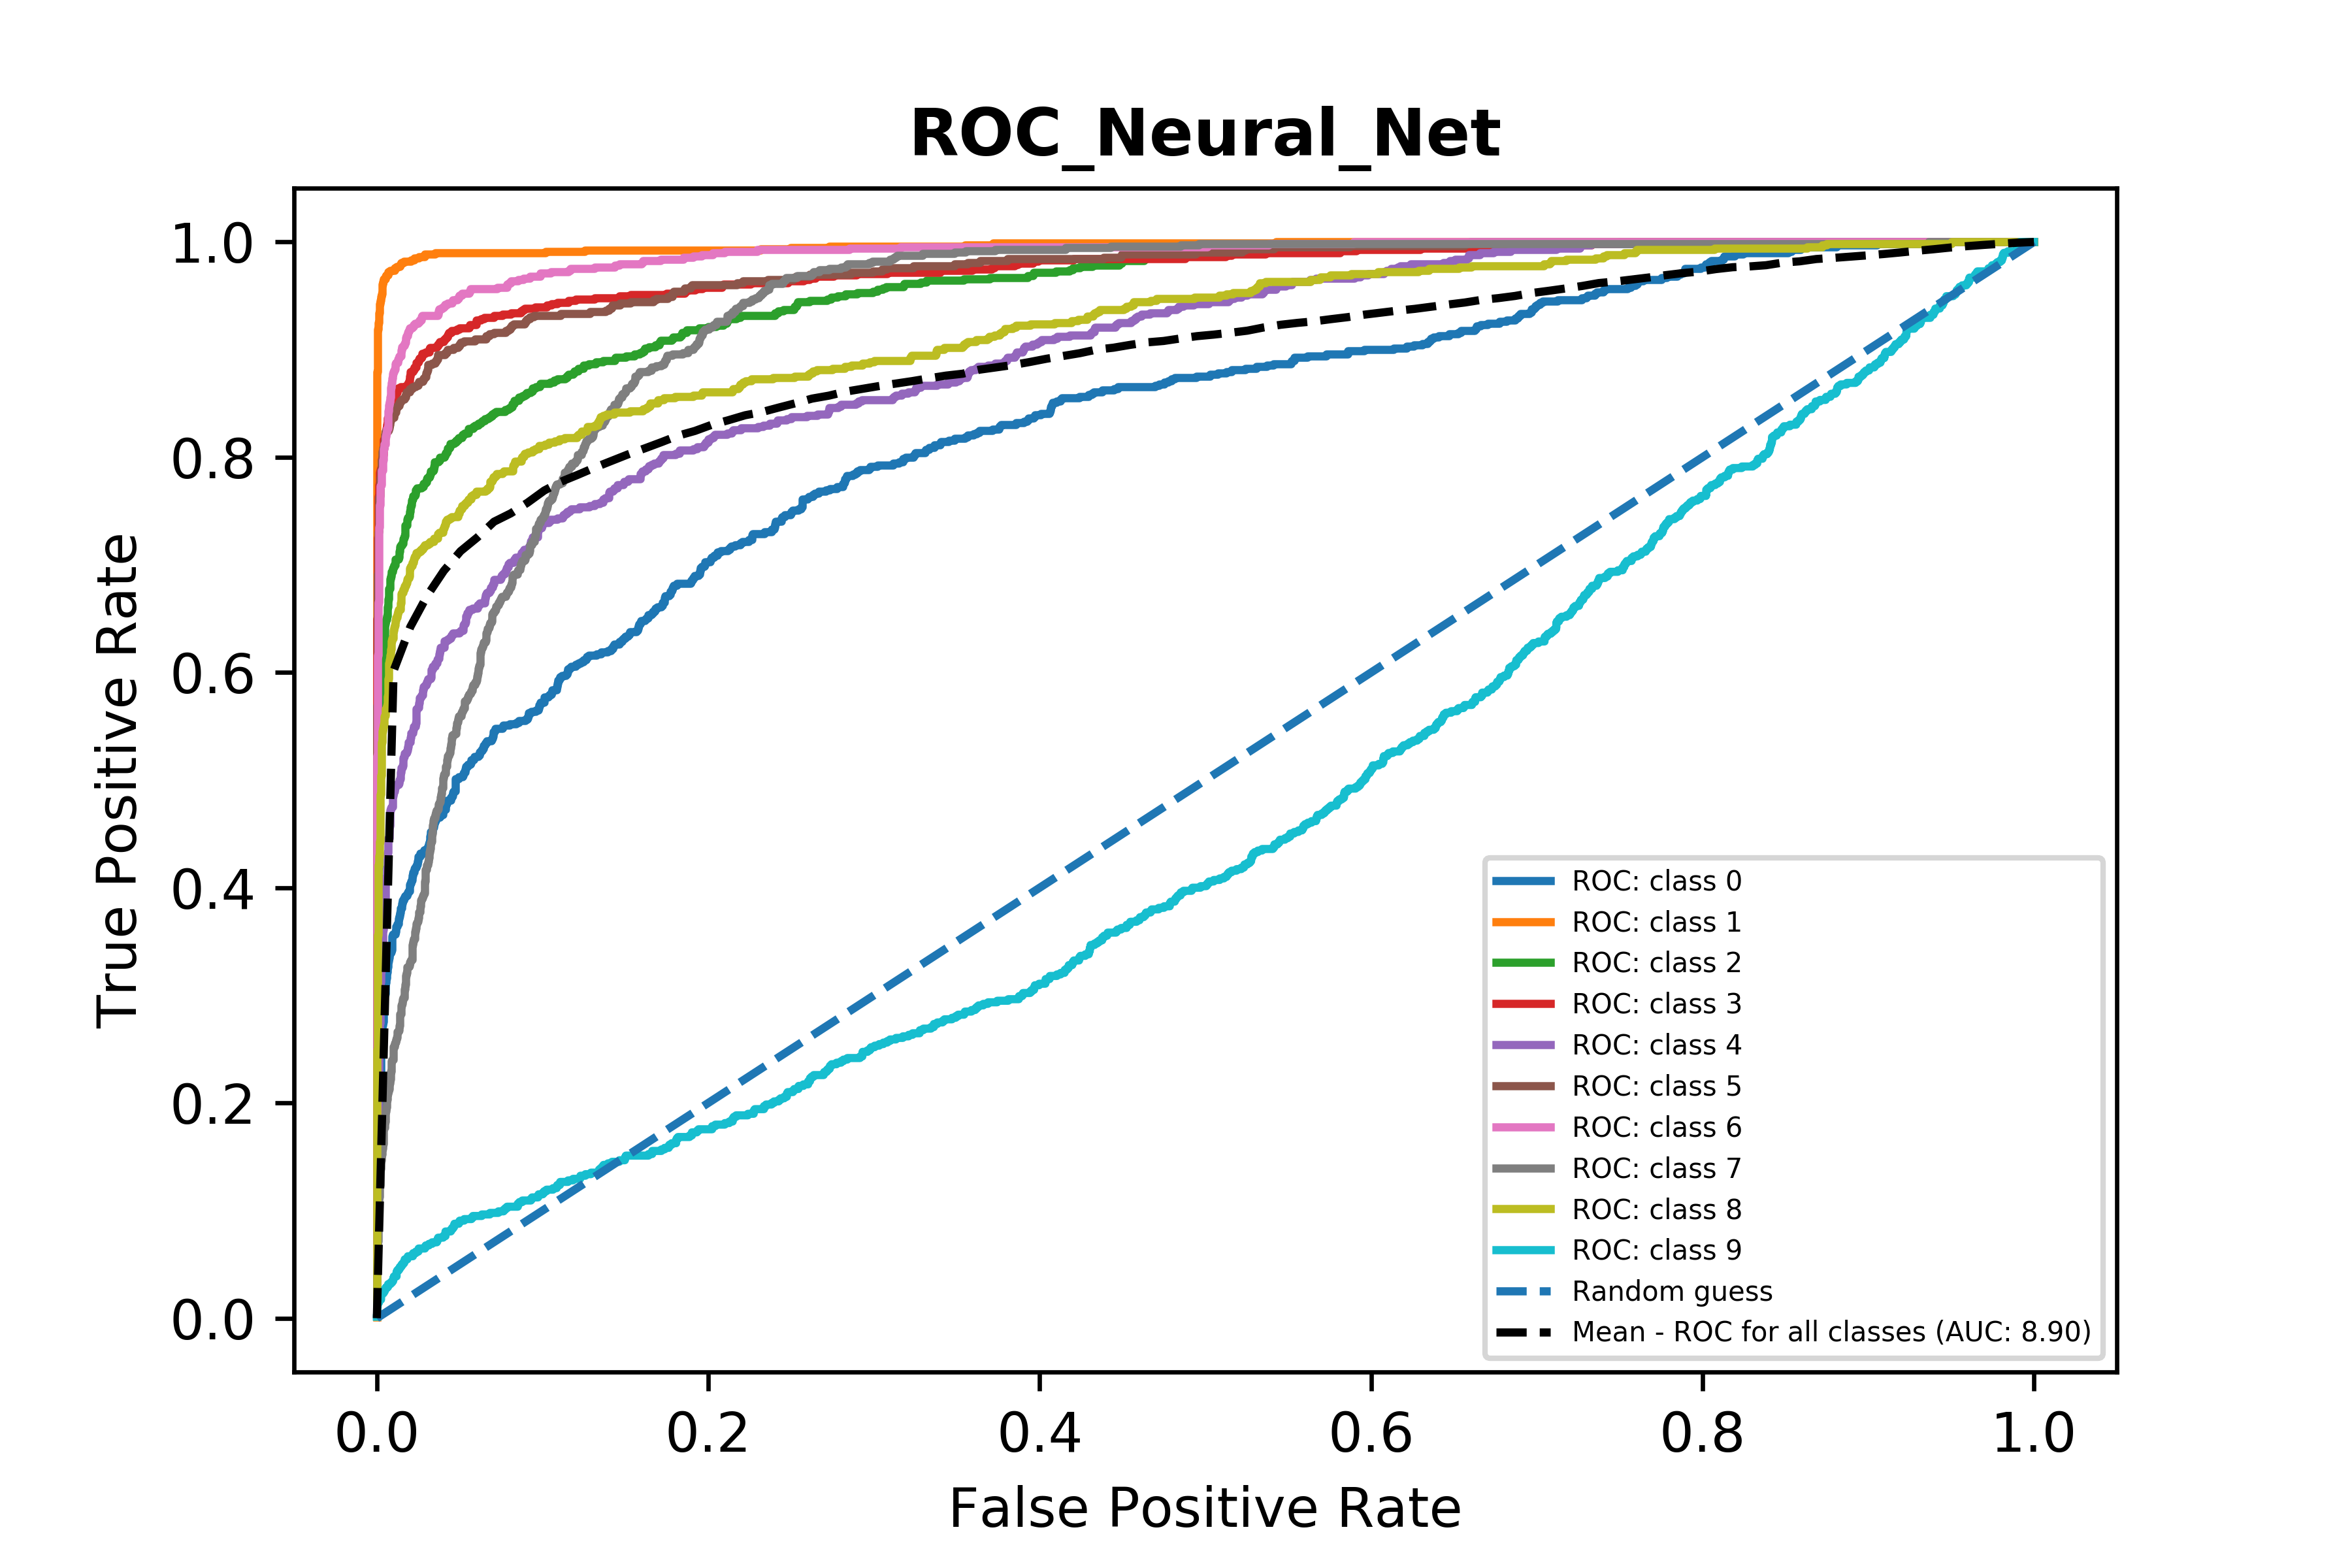
\includegraphics[width=0.6\linewidth]{figures/roc_example.png}
\caption{ROC curve example \label{fig:roc_eg}}
\end{figure}

\addcontentsline{toc}{subsubsection}{Confusion matrices}
\subsubsection*{Confusion matrices}

Confusion matrices are another way to study the performance of a classification algorithm. While the configuration of a confusion matrix is straightforward for a binary classification, for multi-class classification it can be represented as a matrix of values of size $(n \times n)$, where $n$ is the number of classes.

An example of a confusion matrix for the MNIST dataset is shown in Fig. \ref{fig:conf_eg}. The confusion matrix is being plotted as a colormap using the in-built capabilities of \texttt{matplotlib} Python package and each row represents the proportion of classification of each class being classified as different classes by a classifier. For a perfect classifier, the confusion matrix would be an identity matrix.

\begin{figure}[H]
\centering
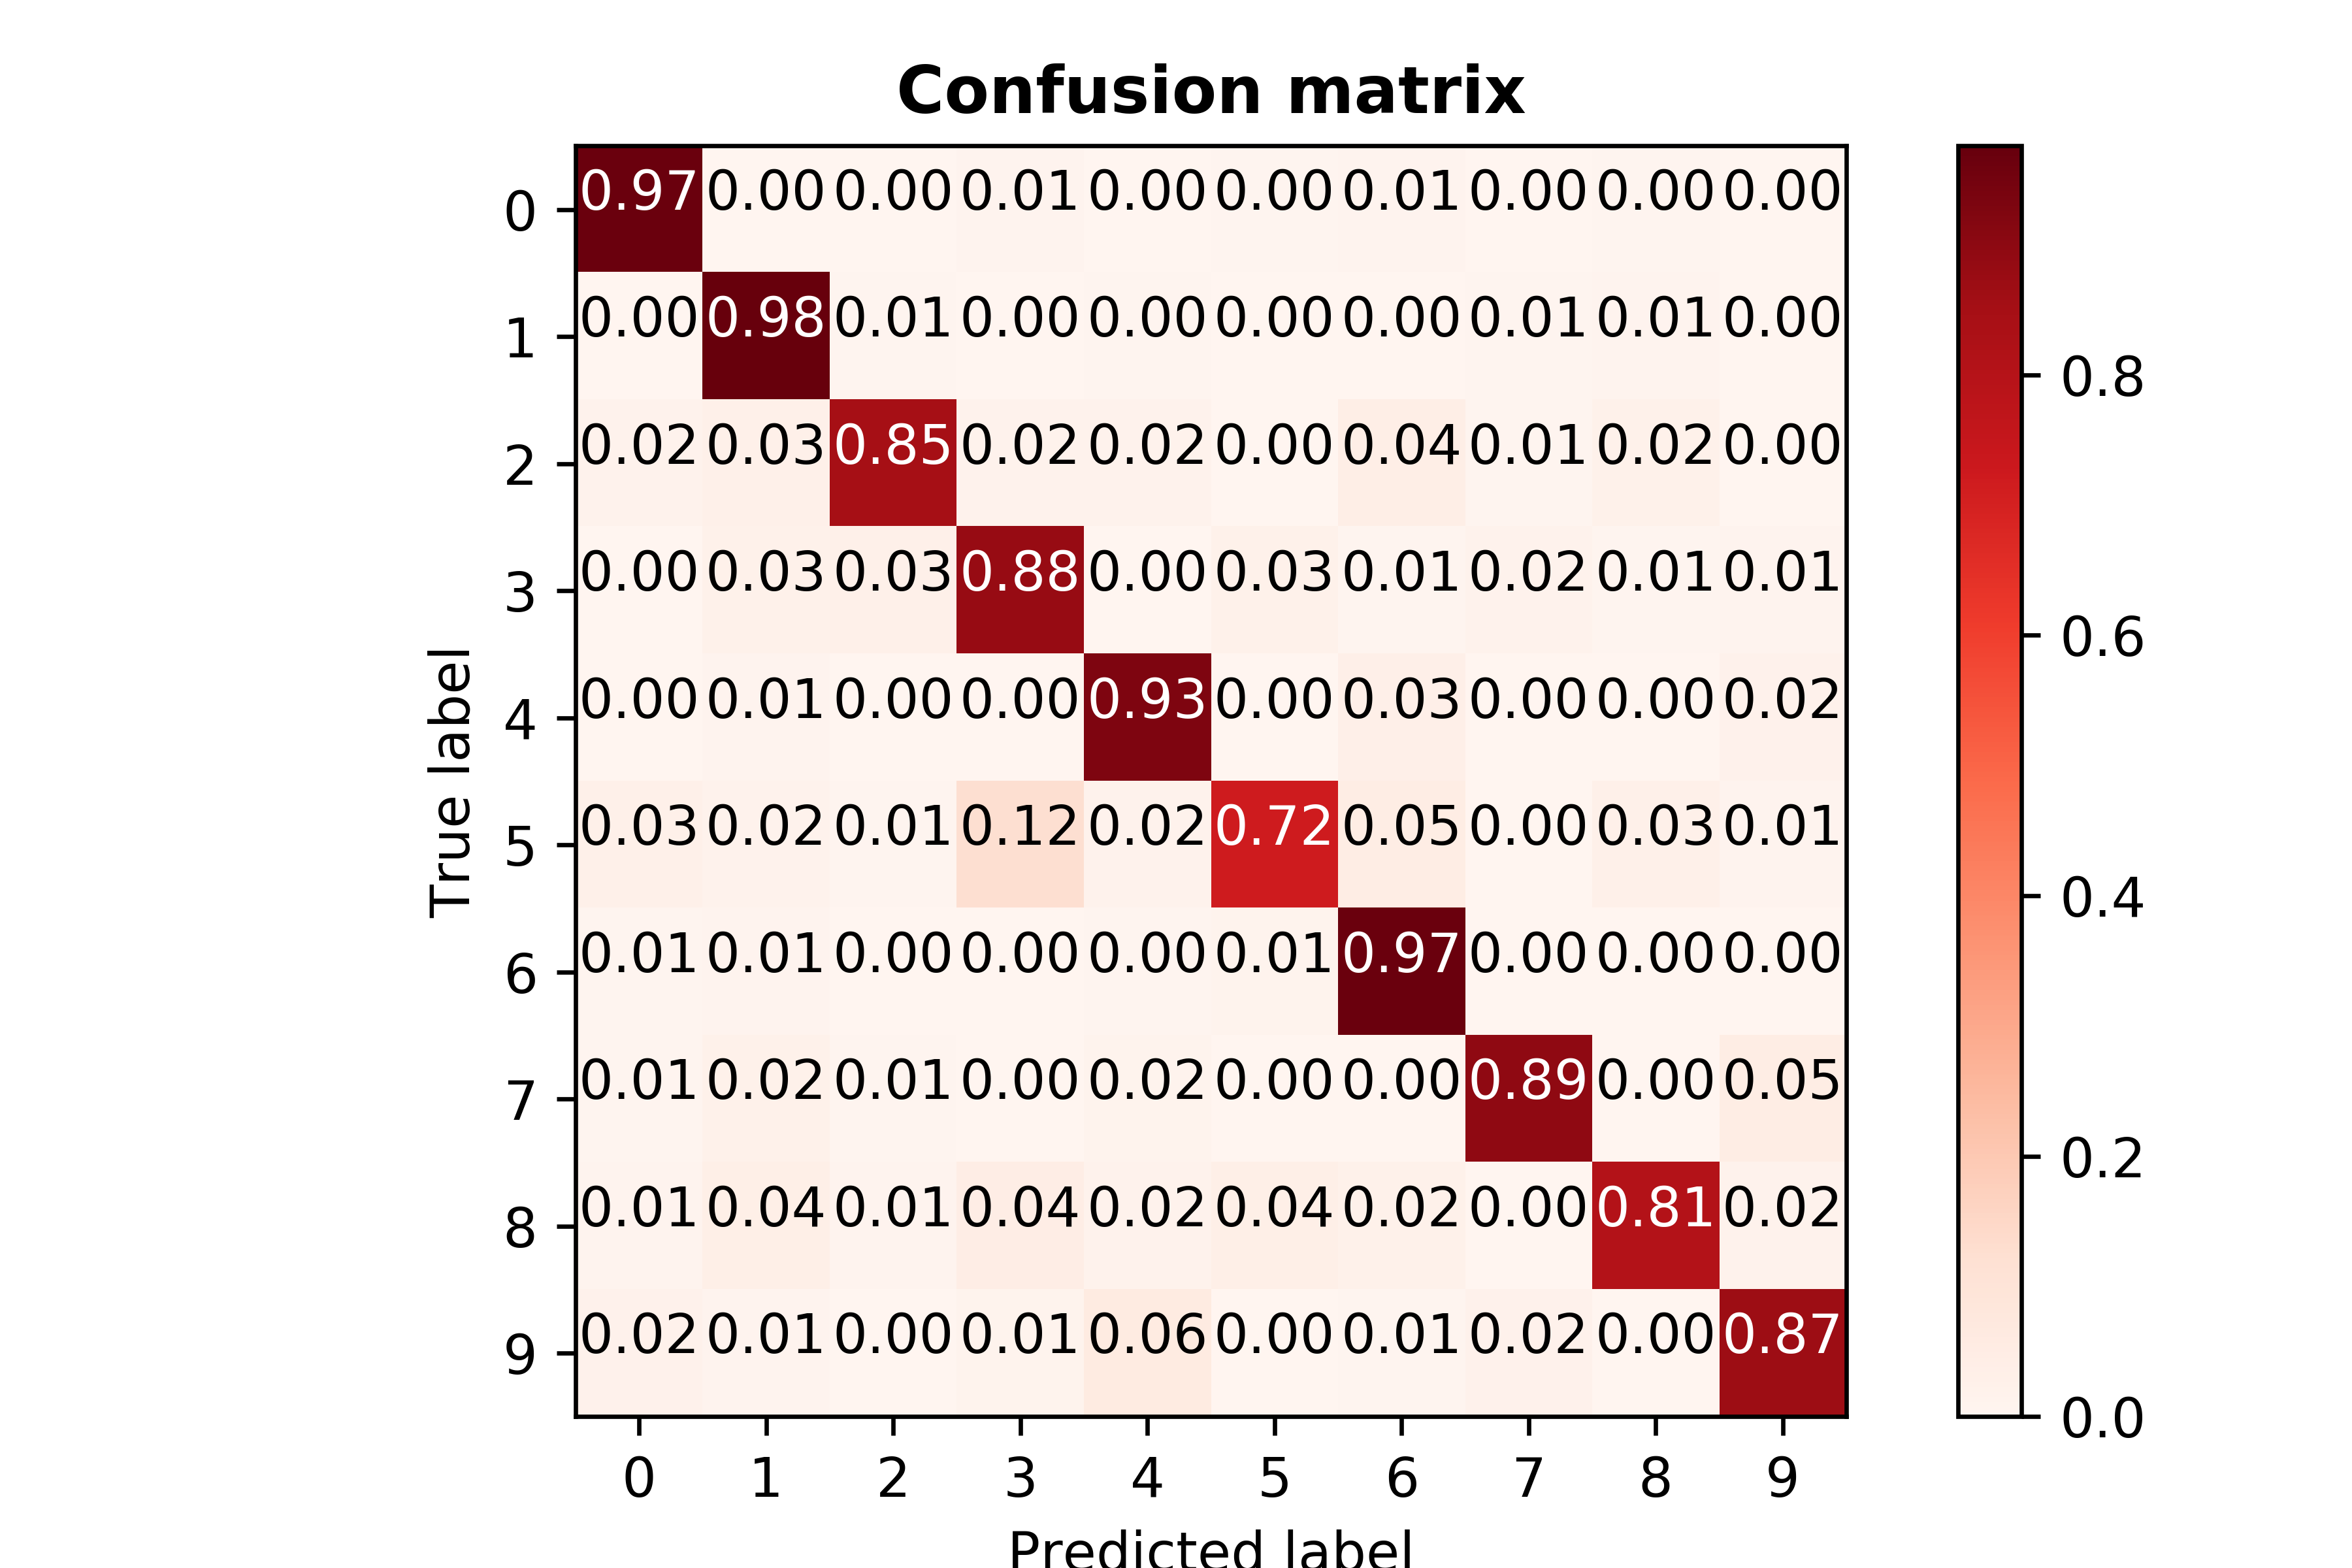
\includegraphics[width=0.6\linewidth]{figures/confusion_example.png}
\caption{Confusion matrix example \label{fig:conf_eg}}
\end{figure}

\addcontentsline{toc}{subsubsection}{Accuracy curve}
\subsubsection*{Accuracy curve}
As part of the experiments, we perform a 10-fold cross validation for parameter tuning, for hypothesis testing, etc. and to study the performance of algorithms in these tests, we study the accuracy score in the test fold. Since this is a multi-class classification, the accuracy of the model is represented as:

\begin{equation*}
Accuracy = \frac{True\_Positives}{Total\_number\_of\_samples}
\end{equation*}

Once we have this information, the plot showing the variation of accuracy with varying parameters were plotted as error bars (containing both mean and variance information) and these have been included in the results section.

\addcontentsline{toc}{subsubsection}{Hypothesis testing}
\subsubsection*{Hypothesis testing}
Once we had all these performance metrics, we compared the performance of algorithms using hypothesis testing. The data from the 10-fold CV steps were used for comparing the algorithms. Given a pair of means $(\mu_{1}, \mu_{2})$ and variances $(\sigma_1,\sigma_2)$, we determine:

\begin{equation*}
x = \frac{(\hat{\mu_1} - \hat{\mu_2})\sqrt{n}}{\sqrt{\hat{\sigma_1}^{2} + \hat{\sigma_2}^{2}}}
\end{equation*}

\begin{equation*}
\nu = \ceil*{\frac{{\hat{\sigma_1}^{2} + \hat{\sigma_2}^{2}}^{2}(n-1)}{\hat{\sigma_1}^{4} + \hat{\sigma_2}^{4}}}
\end{equation*}

From these values, we reject the null hypothesis $\mu_1 = \mu_2$, in favor of $\mu_1 > \mu_2$, if $x > x_{1-\alpha, \nu}$. We fixed the confidence level $\alpha = 0.95$. In our case, we performed hypothesis testing for comparing the following pairs of algorithms:

\begin{itemize}
\item SVM vs. Neural Net (using PCA data)
\item SVM vs. KNN (using PCA data)
\item Neural Net vs. KNN (using PCA data)
\item SVM vs. Neural Net (using actual data)
\item SVM vs. KNN (using actual data)
\item Neural Net vs. KNN (using actual data)
\item SVM (with PCA) vs. SVM (without PCA)
\item Neural Net (with PCA) vs. Neural Net (without PCA)
\item KNN (with PCA) vs. KNN (without PCA)
\end{itemize}

All of these hypothesis tests were done with the results from the 10-fold cross validation (which use the tuned parameters that were found earlier using the parameter tuning experiments explained earlier). So, in a sense each algorithm is performing at it's best for the MNIST dataset. Of course, considering more parameters and tuning within a finer range of these parameters might result in better performance of the respective algorithms.  

\addcontentsline{toc}{subsubsection}{Principal Component Analysis (PCA)}
\subsubsection*{Principal Component Analysis (PCA)}
Principal Component Analysis (PCA) is a common dimensionality reduction procedure that is used in statistics / machine learning for high dimensional data. After finding the principal components, we can select a few components in the order of maximum variance along these components and project the training data into this subspace.

When a test data point comes in, we project it to the previously mentioned subspace and use the dimensionally reduced form of the data for prediction. We used this procedure for a few experiments as explained in the upcoming sections, albeit with a few considerations to make sure that we don't use any information from the test data:

\begin{itemize}
\item{\textbf{10-fold cross validation.}} Whenever we perform cross-validation and we use PCA for dimensionality reduction, we make sure that we perform PCA to only the \texttt{9-folds} of data that is being considered as the \texttt{training set}. So the PCA matrix and mean values that are obtained for these data are then used to: \textbf{(i) center} the test data (the remaining 1-fold) and \textbf{(ii) project} that centered data to the subspace.

\item{\textbf{Centering the data.}} The centering of the data is done only for the training set and the same mean is used for the test set to ensure that the data is being processed with respect to the same origin in the subspace
\end{itemize}
 
\addcontentsline{toc}{subsubsection}{Other Miscellaneous Metrics}
\subsubsection*{Other Miscellaneous Metrics} 
Apart from these parameters, we also report Precision and Recall scores for the final test runs (10-fold CV using the tuned parameters). While precision and recall are not as efficient as accuracy in gauging the performance of an algorithm, they have been included to provide a sense of completion and in understanding the performance from different perspectives. 

Since we use a multi-class dataset, the precision and recall scores have been calculated using a "\textit{weighted-averaging}" technique. Here, the metrics are calculated for each label and a weighted average of them is taken based on the support (the number of samples for each label in the dataset).


\addcontentsline{toc}{section}{Experiments/Results}
\section*{Experiments/Results} 

\addcontentsline{toc}{subsection}{10-Fold Cross Validation For Parameter Tuning}
\subsection*{10-Fold Cross Validation For Parameter Tuning}

For 10-fold cross validation we used stratified sampling using all 70,000 MNIST data. We first divided the whole data into 10 groups (data belonging to each digit from 0-9). Then  for each fold in 10-fold CV, we picked one fold from each group and combined them to form our test data set (approximately 7,000 data points) and rest of the data i.e. the other 9-folds were our training data set (approximately 63,000 data points). 

\addcontentsline{toc}{subsubsection}{Support Vector Machines}
\subsubsection*{Support Vector Machines}
The results for SVM is shown in Fig. \ref{fig:svm_cv_param}. The figure shows the trend for ``\textit{Accuracy}'' as we vary the regularization parameter (C) for SVM. The plot shows both the mean and the variance of the accuracy values (from the cross-validation for each value of `C'). 

\paragraph{Observations.}
The C parameter is a measure of how much we want to avoid mis-classifying each training example. Large values of C will result in the hyperplane having a smaller margin and in cases where the data is separable, this would usually results in a better performing SVM with lesser misclassifications. Conversely, a a small value of C will cause the optimizer to look for a larger-margin separating hyperplane, even if that hyperplane misclassifies more points. 

\begin{figure}[H]
\centering
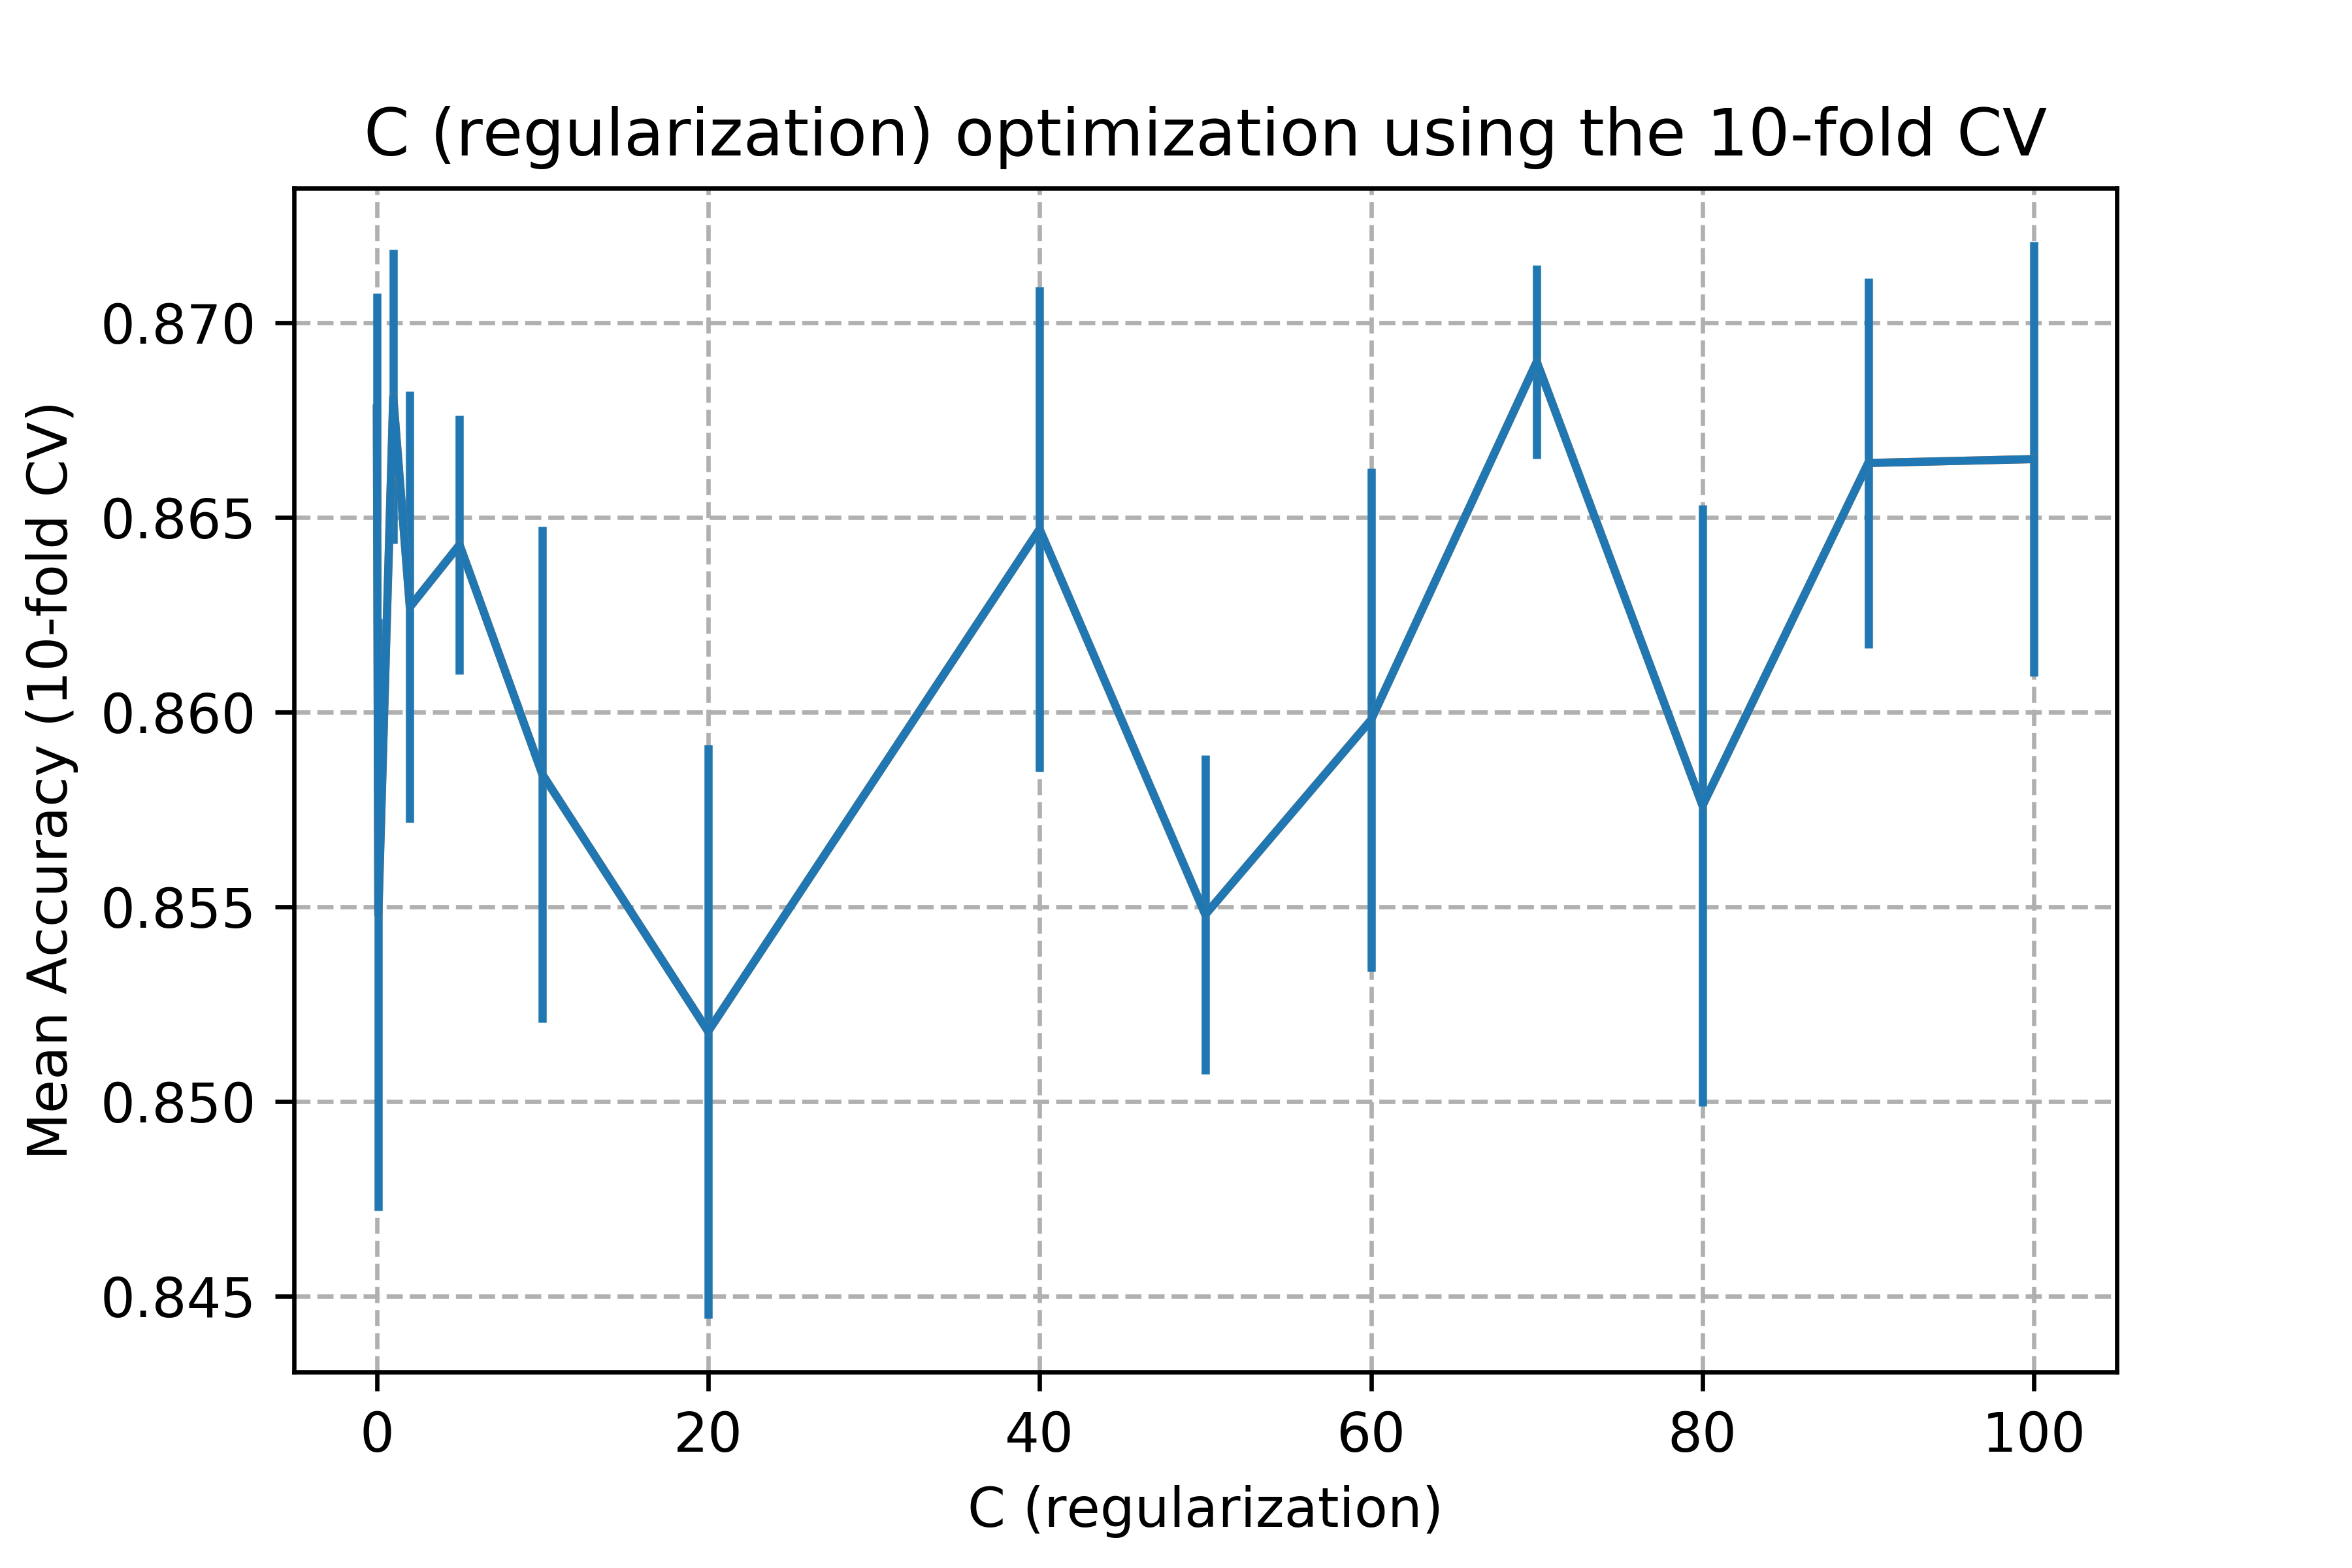
\includegraphics[width=0.6\linewidth]{figures/SVM_regularization_C_mean_acc_error_bar.png}
\caption{10-fold CV (Parameter tuning) for SVM \label{fig:svm_cv_param}}
\end{figure}

An interesting thing that we observed while tuning the parameter `C' for our dataset is the \textit{absence} of a clear trend while changing the parameter value. As can be seen from the plot, we had a higher density of values for `C' at the lower range in order to study the effect of the parameter better. However, the trend of the variance and mean in accuracy suggests that the data (MNIST) is \textbf{\textit{not linearly separable}} causing the hyperplane to misclassify points even at high values of `C' and hence the effect of C is very minimal in this dataset. 

\begin{figure}
\centering
\includegraphics[width=0.5\linewidth]{figures/{SVM_linear_ROC_C_0.01_k_1}.png}%
\includegraphics[width=0.5\linewidth]{figures/{SVM_linear_ROC_C_2.0_k_1}.png}%
\linebreak
\includegraphics[width=0.5\linewidth]{figures/{SVM_linear_ROC_C_40.0_k_1}.png}%
\includegraphics[width=0.5\linewidth]{figures/{SVM_linear_ROC_C_70.0_k_1}.png}%
\linebreak
\includegraphics[width=0.5\linewidth]{figures/{SVM_linear_ROC_C_100.0_k_1}.png}%
\caption{ROC curves with AUC for the mean curve for $C = 0.01, 2, 40, 70, 100$ (Going from Left to Right and Top to Bottom)} 
\label{fig:roc_c_svm}
\end{figure}

After performing these experiments, the hyper-parameter C for SVM was selected to be $\mathbf{70}$. This was the highest value in the plot and hence was chosen even though the trend does not suggest an obvious answer. Apart from the accuracy curve, the performance was also studied using ROC curves while changing the values of `C'. The results are shown in Fig. \ref{fig:roc_c_svm} for a few values of C. Along with the ROC curves, the Area Under Curve (AUC) metric is also included for the mean curve (which was found using the ``macro-averaging'' approach). The plots shown are all for the $1^{st}$ fold of the cross validation experiment. The plots for all the folds and for the entire range of the parameter is included in the submission folder. 

\addcontentsline{toc}{subsubsection}{Neural Networks}
\subsubsection*{Neural Networks}
The results for Neural Networks is shown in Fig. \ref{fig:nn_cv}. Unlike SVM, where we just looked at one parameter to optimize, we optimized the neural net that we chose using three different parameters namely: the \texttt{activation function}, the \texttt{learning rate} for the backpropagation algorithm, and the regularization parameter $\mathtt{\alpha}$.

\paragraph{Observations.}

\begin{itemize}
\item{\textbf{Activation function.}} We looked at three options for the activation function for the neurons in the NN: The logistic sigmoid function (\textbf{logistic}), the hyperbolic tan function (\textbf{tanh}) and the rectified linear unit function (\textbf{relu}). While the \textbf{relu} function just a max classifier ($f(x)=max(0,x)$), the other two are more involved and thus we expect better accuracy, which is the case as can be seen from the Figure. After running the CV, we chose the \textbf{logistic} activation function based on the results.

\begin{figure}[H]
\centering
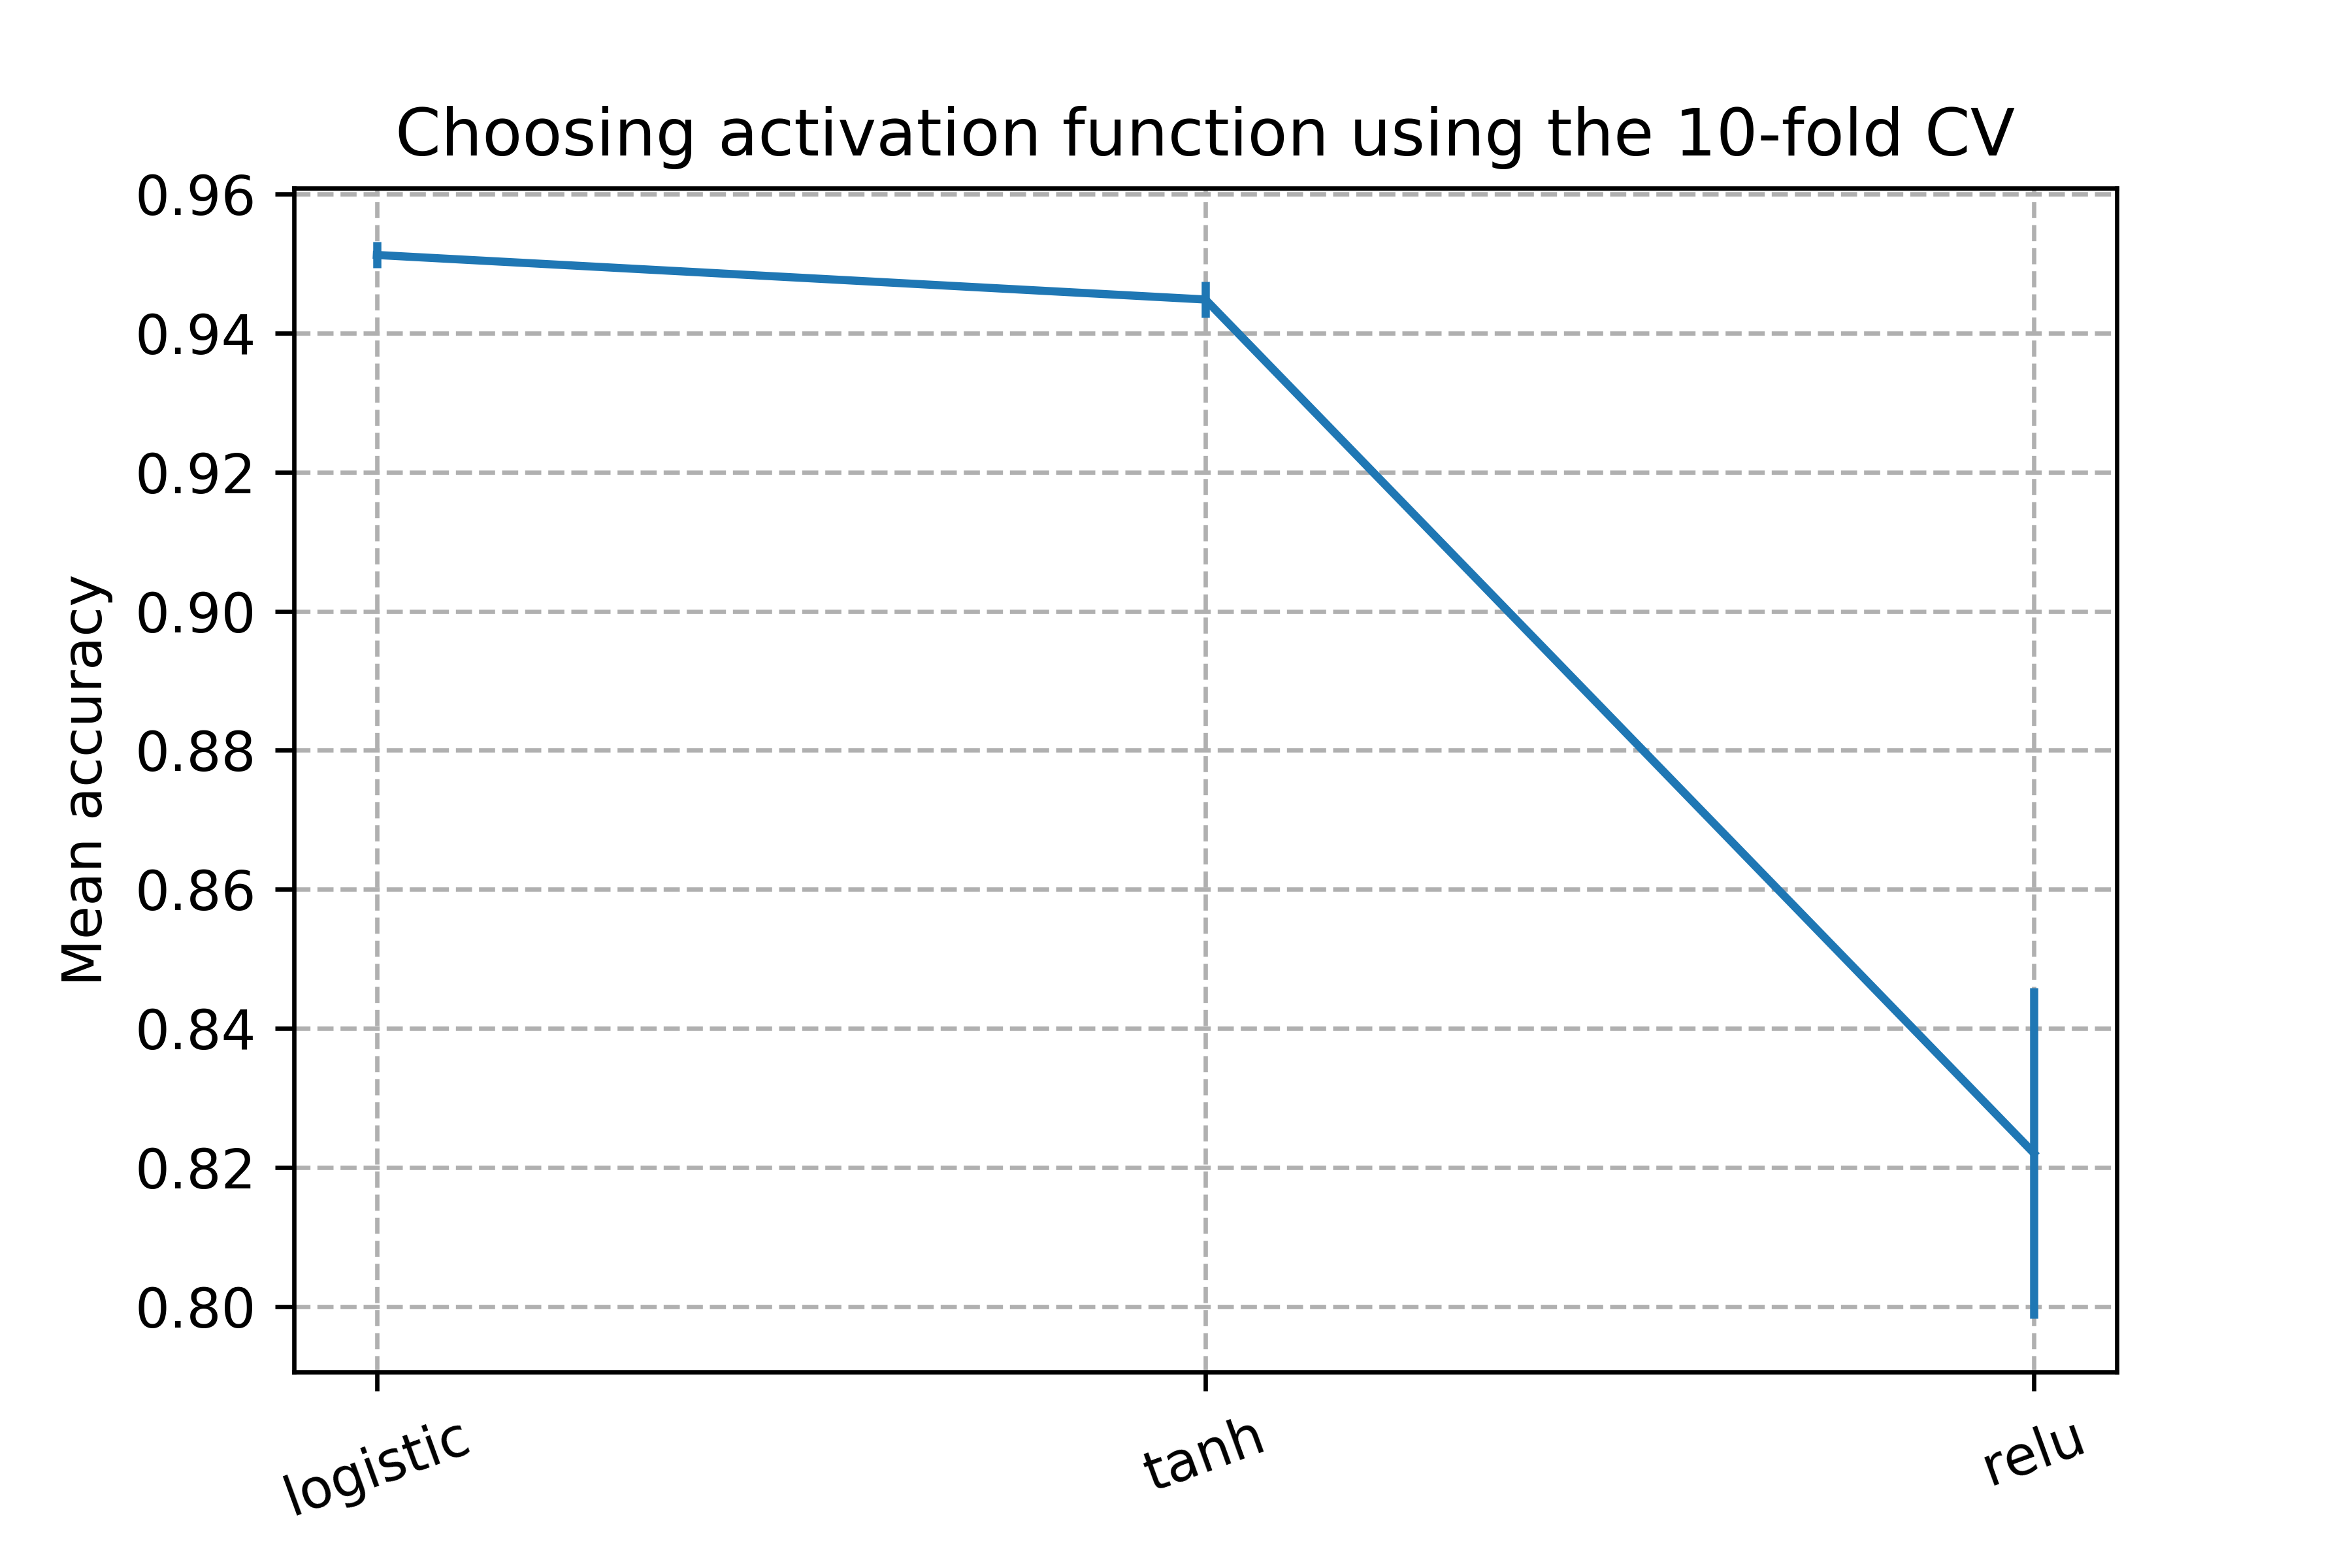
\includegraphics[width=0.5\linewidth]{figures/Neural_net_act_fcn_mean_acc_error_bar.png}%
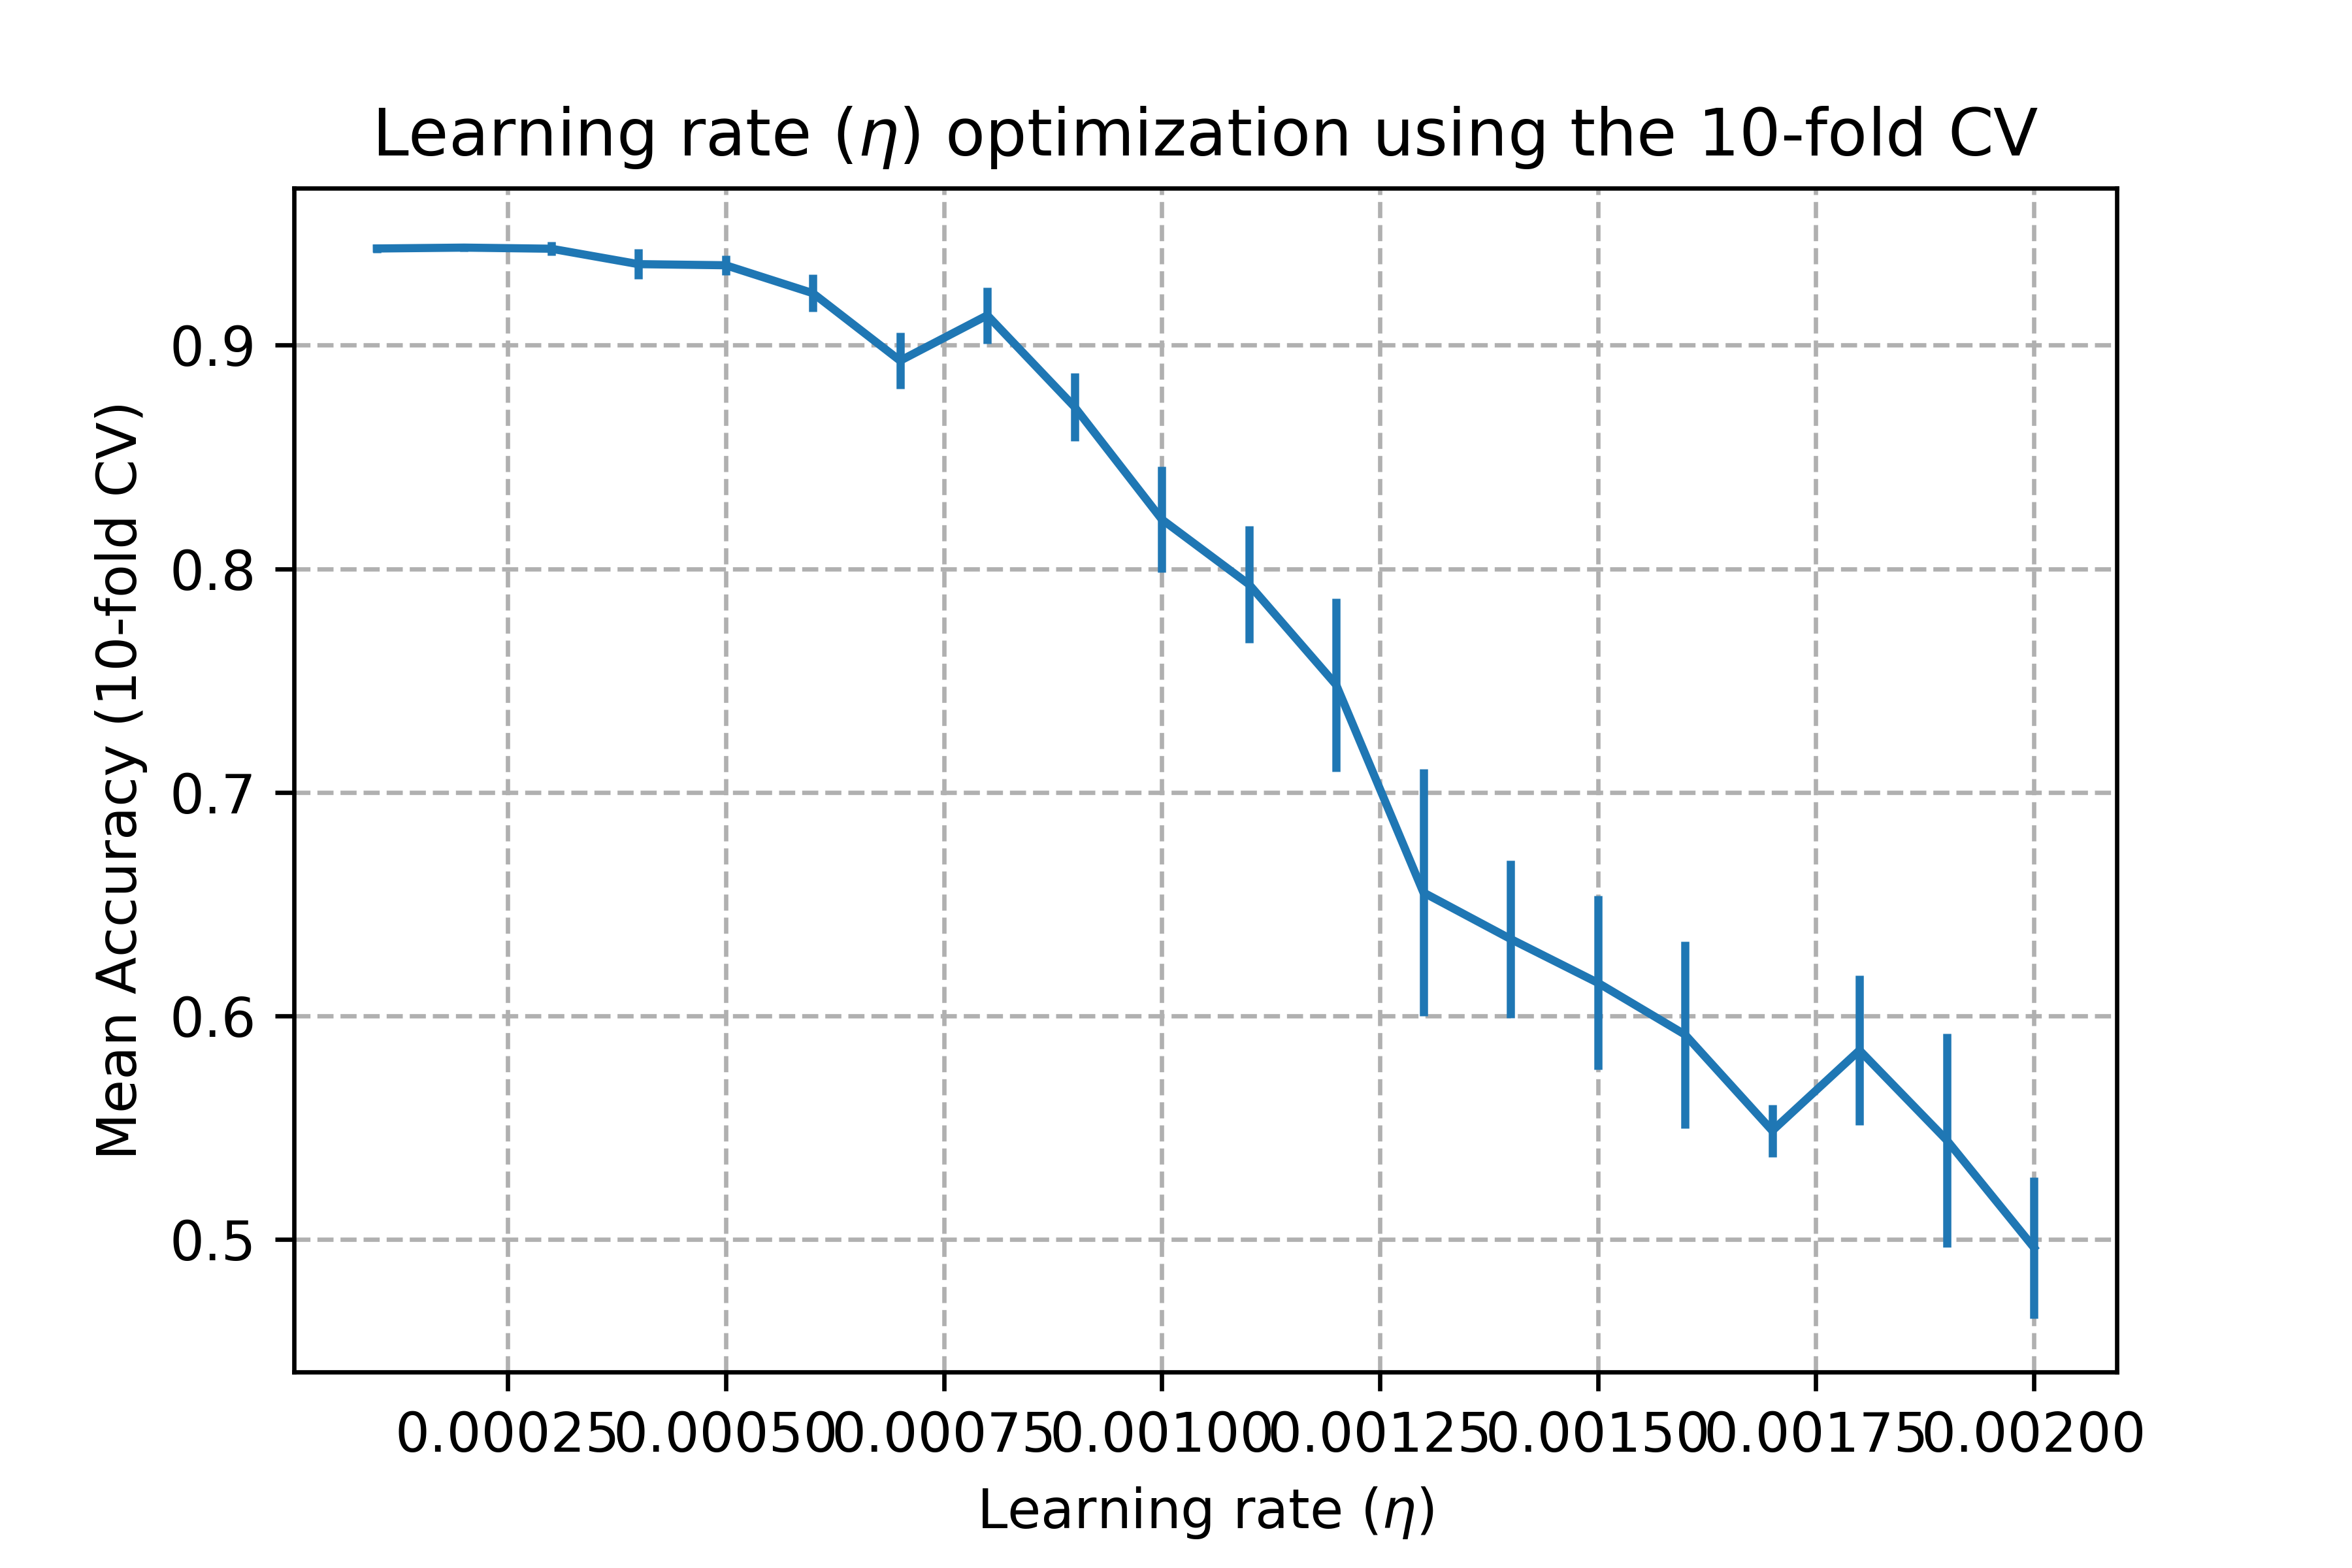
\includegraphics[width=0.5\linewidth]{figures/Neural_net_learn_rate_mean_acc_error_bar.png} %
\linebreak 
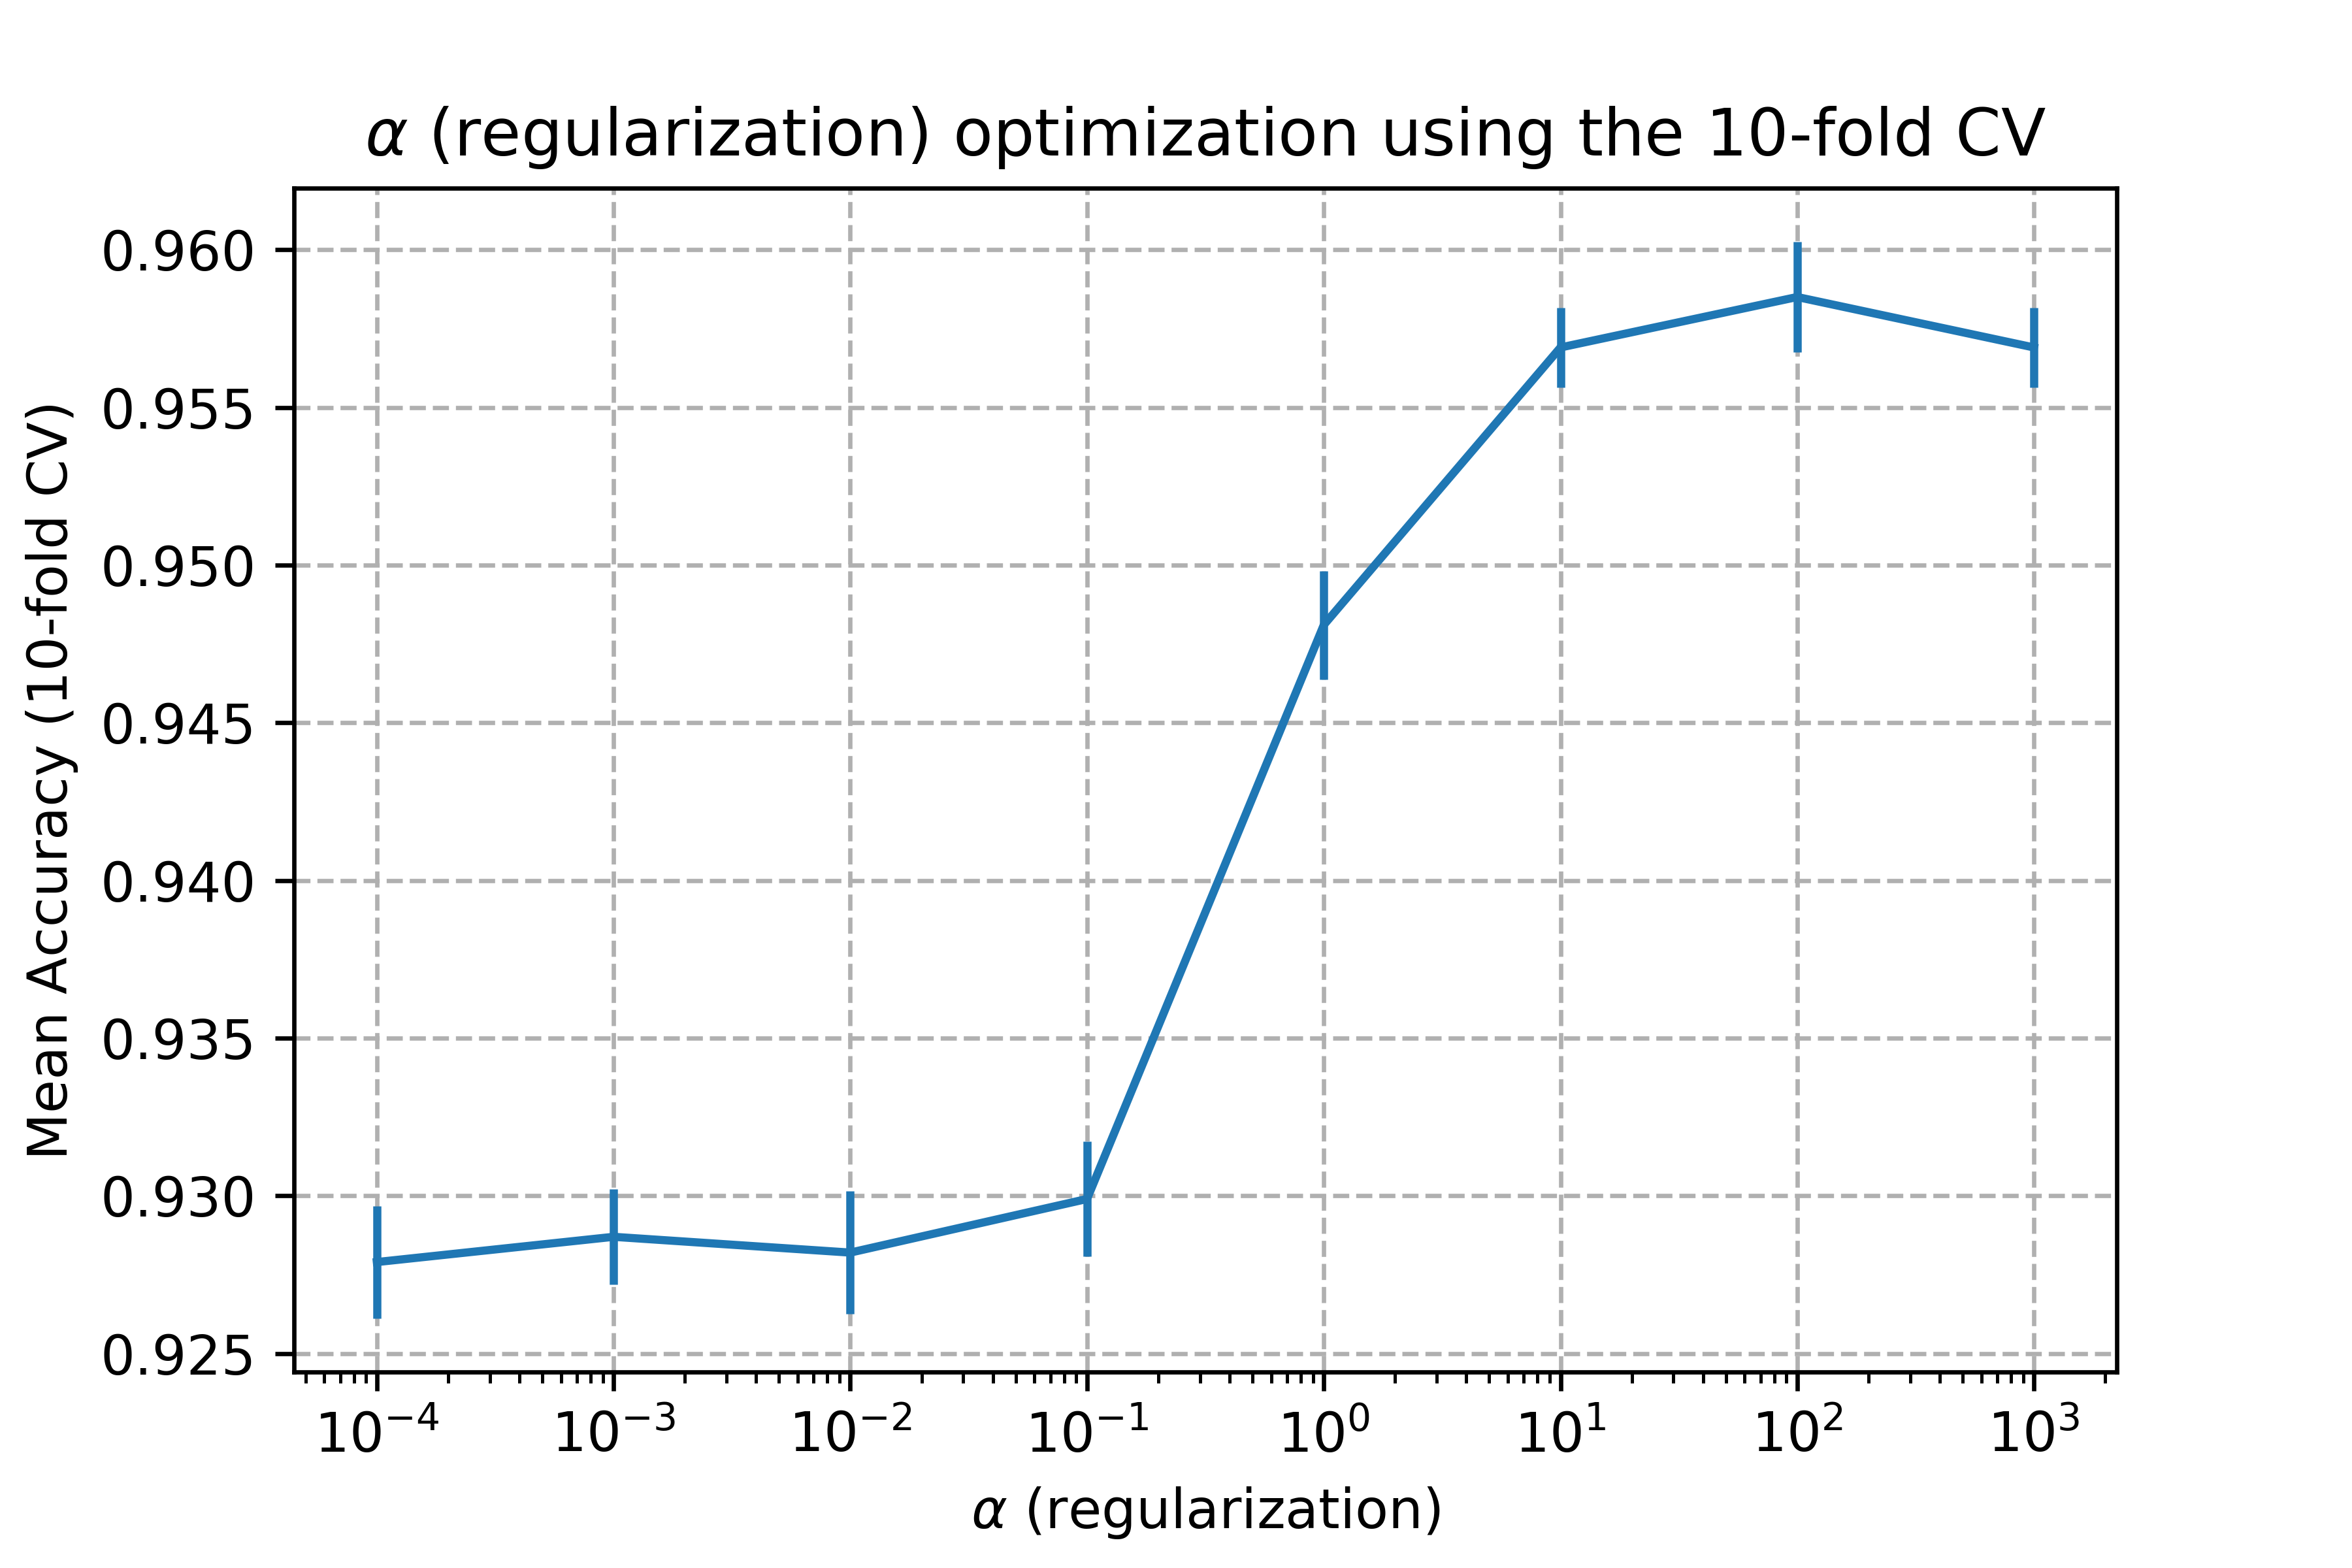
\includegraphics[width=0.5\linewidth]{figures/Neural_net_alpha_mean_acc_error_bar.png}
\caption{CV for Neural networks. \label{fig:nn_cv}}
\end{figure}

\item{\textbf{Learning rate.}} Learning rate is NN is used to control the convergence to an optimal solution of the cost function. A larger learning rate might converge faster but might overshoot the optimal value, while a lower learning rate might take a long time to converge. Hence, we experimented with a range of values for the tuning, expecting a better accuracy for lower values. And the results met our expectations, giving us the best accuracy for a value of ($\eta$): 0.0003. While this comes at a price of higher training times, the compromise was not significant and in order to demonstrate this, a plot of the training times for the dataset for different values of the learning rate is shown in Fig. \ref{fig:train_time_nn}. 

\begin{figure}[H]
\centering
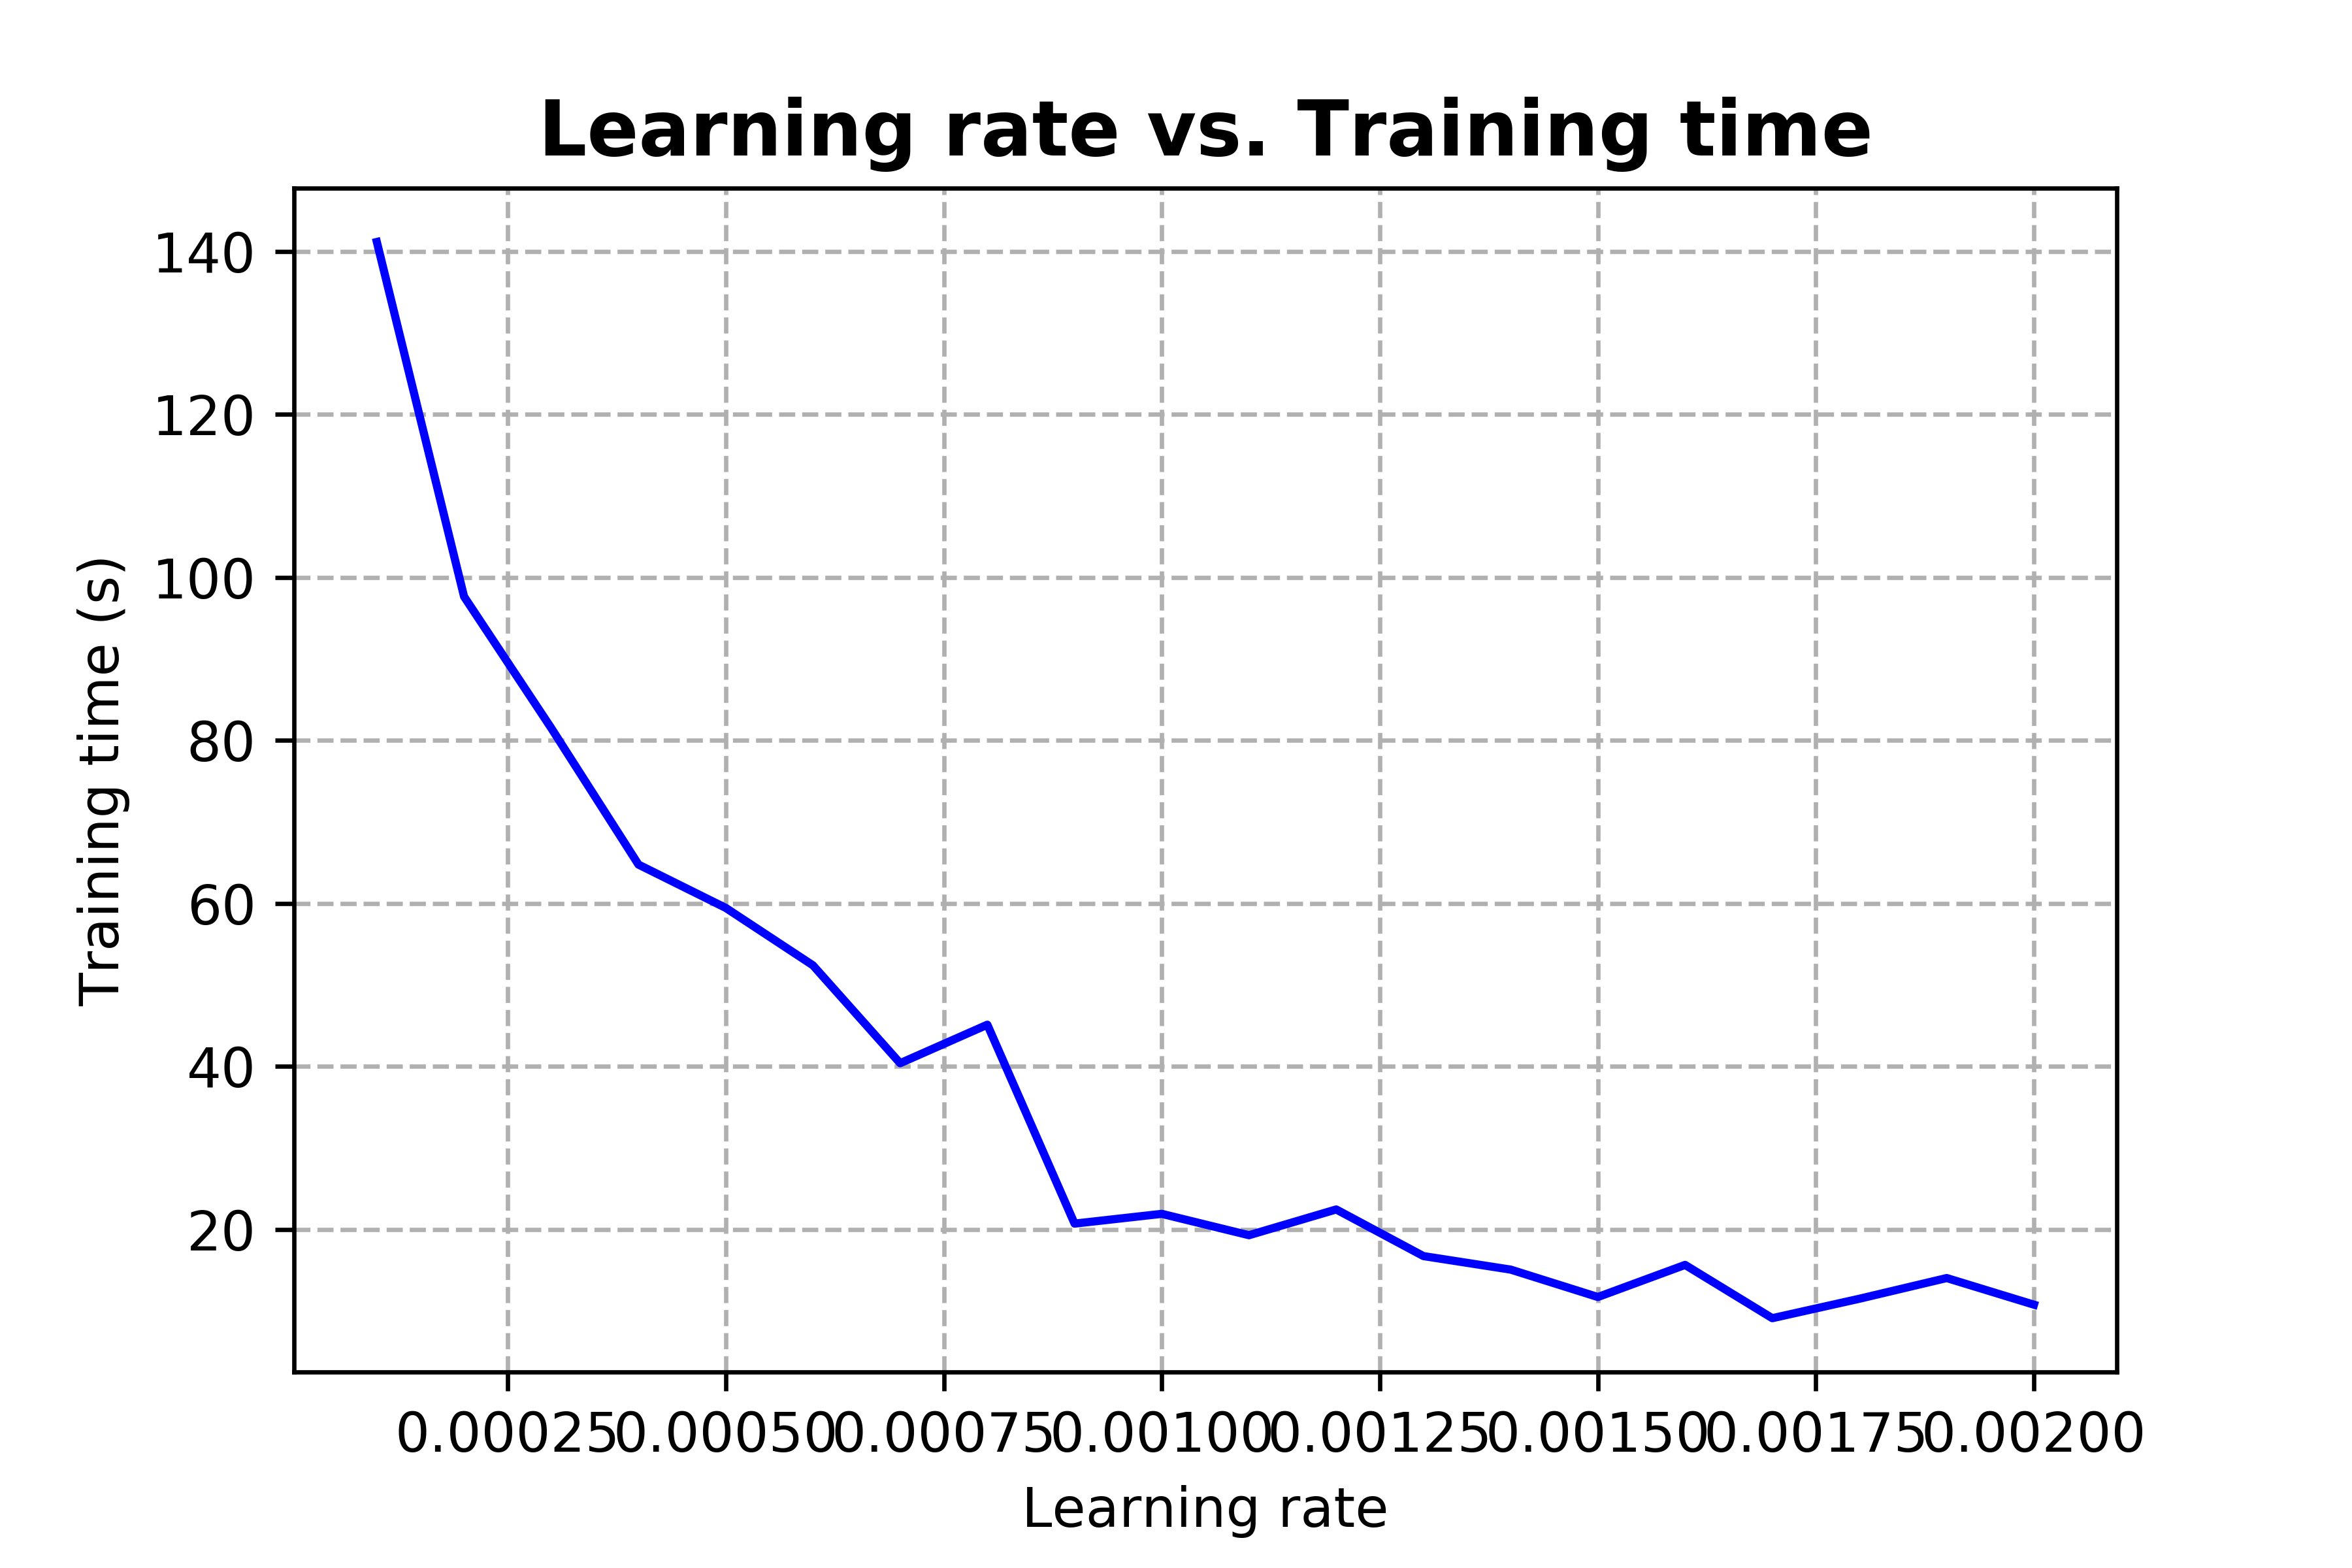
\includegraphics[width=0.6\linewidth]{figures/train_time_learn_rate_nn.png}
\caption{Training time vs. Learn rate \label{fig:train_time_nn}}
\end{figure}

\item{\textbf{Regularization parameter:}} Like any other learning algorithm, the regularization parameter here helps in reducing an \textbf{overfit} of the training data and having the trained algorithm to have a robust classifying behavior when it sees the test data. We used a range of values, and in order to have a bigger picture of the effect of the parameter, a \textbf{logscale} was used as shown in Fig. \ref{fig:nn_cv}. From these observations, a value of ($\alpha$): $100$ is picked as the best tuned parameter.  
  
\begin{figure}
\centering
\includegraphics[width=0.5\linewidth]{figures/{Neural_Net_linear_ROC_Alpha_0.0001_k_1}.png}%
\includegraphics[width=0.5\linewidth]{figures/{Neural_Net_linear_ROC_Alpha_0.001_k_1}.png}%
\linebreak
\includegraphics[width=0.5\linewidth]{figures/{Neural_Net_linear_ROC_Alpha_1.0_k_1}.png}%
\includegraphics[width=0.5\linewidth]{figures/{Neural_Net_linear_ROC_Alpha_100.0_k_1}.png}%
\linebreak
\includegraphics[width=0.5\linewidth]{figures/{Neural_Net_linear_ROC_Alpha_10000.0_k_1}.png}%
\caption{ROC curves with AUC for the mean curve for $\alpha = 10^{-5}, 10^{-4}, 10^{-1}, 10^{2}, 10^{3}$ (Going from Left to Right and Top to Bottom)} 
\label{fig:roc_alp_nn}
\end{figure}

\begin{figure}
\centering
\includegraphics[width=0.5\linewidth]{figures/{Neural_Net_linear_ROC_Learn_rate_0.0001_k_1}.png}%
\includegraphics[width=0.5\linewidth]{figures/{Neural_Net_linear_ROC_Learn_rate_0.0005_k_1}.png}%
\linebreak
\includegraphics[width=0.5\linewidth]{figures/{Neural_Net_linear_ROC_Learn_rate_0.0011_k_1}.png}%
\includegraphics[width=0.5\linewidth]{figures/{Neural_Net_linear_ROC_Learn_rate_0.0015_k_1}.png}%
\linebreak
\includegraphics[width=0.5\linewidth]{figures/{Neural_Net_linear_ROC_Learn_rate_0.0019_k_1}.png}%
\caption{ROC curves with AUC for the mean curve for $Learn\_rate = 10^{-5}, 5^{-5}, 11^{-4}, 15^{-4}, 19^{-4}$ (Going from Left to Right and Top to Bottom)} 
\label{fig:roc_lr_nn}
\end{figure}

\begin{figure}
\centering
\includegraphics[width=0.5\linewidth]{figures/{Neural_Net_linear_ROC_Activation_fcn_logistic_k_1}.png}%
\includegraphics[width=0.5\linewidth]{figures/{Neural_Net_linear_ROC_Activation_fcn_relu_k_1}.png}%
\linebreak
\includegraphics[width=0.5\linewidth]{figures/{Neural_Net_linear_ROC_Activation_fcn_tanh_k_1}.png}%
\caption{ROC curves with AUC for the mean curve for Activation\_funciton = \texttt{logistic},\texttt{relu} and \texttt{tanh} (Going from Left to Right and Top to Bottom)} 
\label{fig:roc_act_nn}
\end{figure} 
  
\item{\textbf{Miscellaneous notes.}} Before optimizing these parameters, the size of the neural networks was also decided upon. This was done based on a combination of a review of existing literature for dealing with dataset (and similar datasets) and a set of experiments (refer to the code). After exhaustive experimentation, the size of the neural net was chosen to be $(784,100,10)$, a model which has a single hidden layer with $100$ neural units.	
\end{itemize}


\addcontentsline{toc}{subsubsection}{K-Nearest Neighbors}
\subsubsection*{K-Nearest Neighbors}
The results are shown in Fig. \ref{fig:knn_cv_param}. 

\paragraph{Observations.}
The K parameter in KNN is basically the number of neighbor data points to look at before deciding which class the test point belong to. 

\begin{figure}[H]
\centering
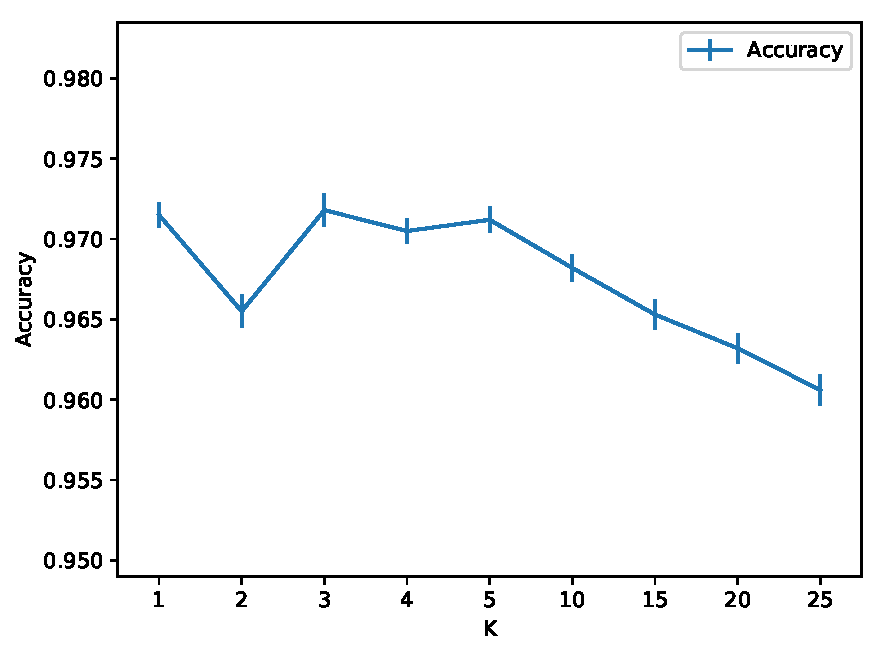
\includegraphics[width=0.4\linewidth]{figures/KNN_accuracy_vs_k_with_all_k_values.pdf}
\caption{10-fold CV for KNN. \label{fig:knn_cv_param}}
\end{figure}

From the figure we observe that the mean accuracy is high at both K=1 and K=3. But since the mean accuracy was little higher at K=3, we chose the value of K to be 3 for KNN. 
We also observe that as we increase the value of K from 3 to to higher number, the accuracy of the test data monotonically decreases. So effect of K is evident from the plot for the MNIST dataset. 

Apart from the accuracy curve, the performance was also studied using ROC curves while changing the values of `K'. The results are shown in Fig. \ref{fig:roc_k_knn} for a few values of K. 

\begin{figure}
\centering
\includegraphics[width=0.5\linewidth]{figures/{KNN_ROC_K_1_fold_1}.pdf}%
\includegraphics[width=0.5\linewidth]{figures/{KNN_ROC_K_3_fold_1}.pdf}%
\linebreak
\includegraphics[width=0.5\linewidth]{figures/{KNN_ROC_K_5_fold_1}.pdf}%
\includegraphics[width=0.5\linewidth]{figures/{KNN_ROC_K_15_fold_1}.pdf}%
\linebreak
\includegraphics[width=0.5\linewidth]{figures/{KNN_ROC_K_25_fold_1}.pdf}%
\caption{ROC curves with AUC for the mean curve for $K = 1,3,5,15,25$ (Going from Left to Right and Top to Bottom)} 
\label{fig:roc_k_knn}
\end{figure} 

\addcontentsline{toc}{subsection}{Effect of number of samples on accuracy}
\subsection*{Effect of number of samples on accuracy}
For this experiment,  we progressively varied the fraction of samples used for training from 1\% to 100\% out of the entire 60,000 samples using randomized stratified sampling, taking the fraction of data from each class (digits 0-9) and combining them to form the training data and computed the accuracy on the test data (fixed size 10,000) for each case. Here we fixed the hyper-parameters for respective algorithm found using CV. The results are shown in Figure \ref{fig:1}.

\textbf{TODO:} Maybe include a paragraph about the implementation / pseudocode for randomized stratified sampling

From the plots we see that, approximately 20\% (12,000) of the training data points (60,000) is required for high accuracy. After 20\% data points, the accuracy almost remains in the same range even if we increase the number of training data points.

\begin{figure}[H]
	\centering
	\begin{subfigure}{0.4\linewidth}
		\centering
		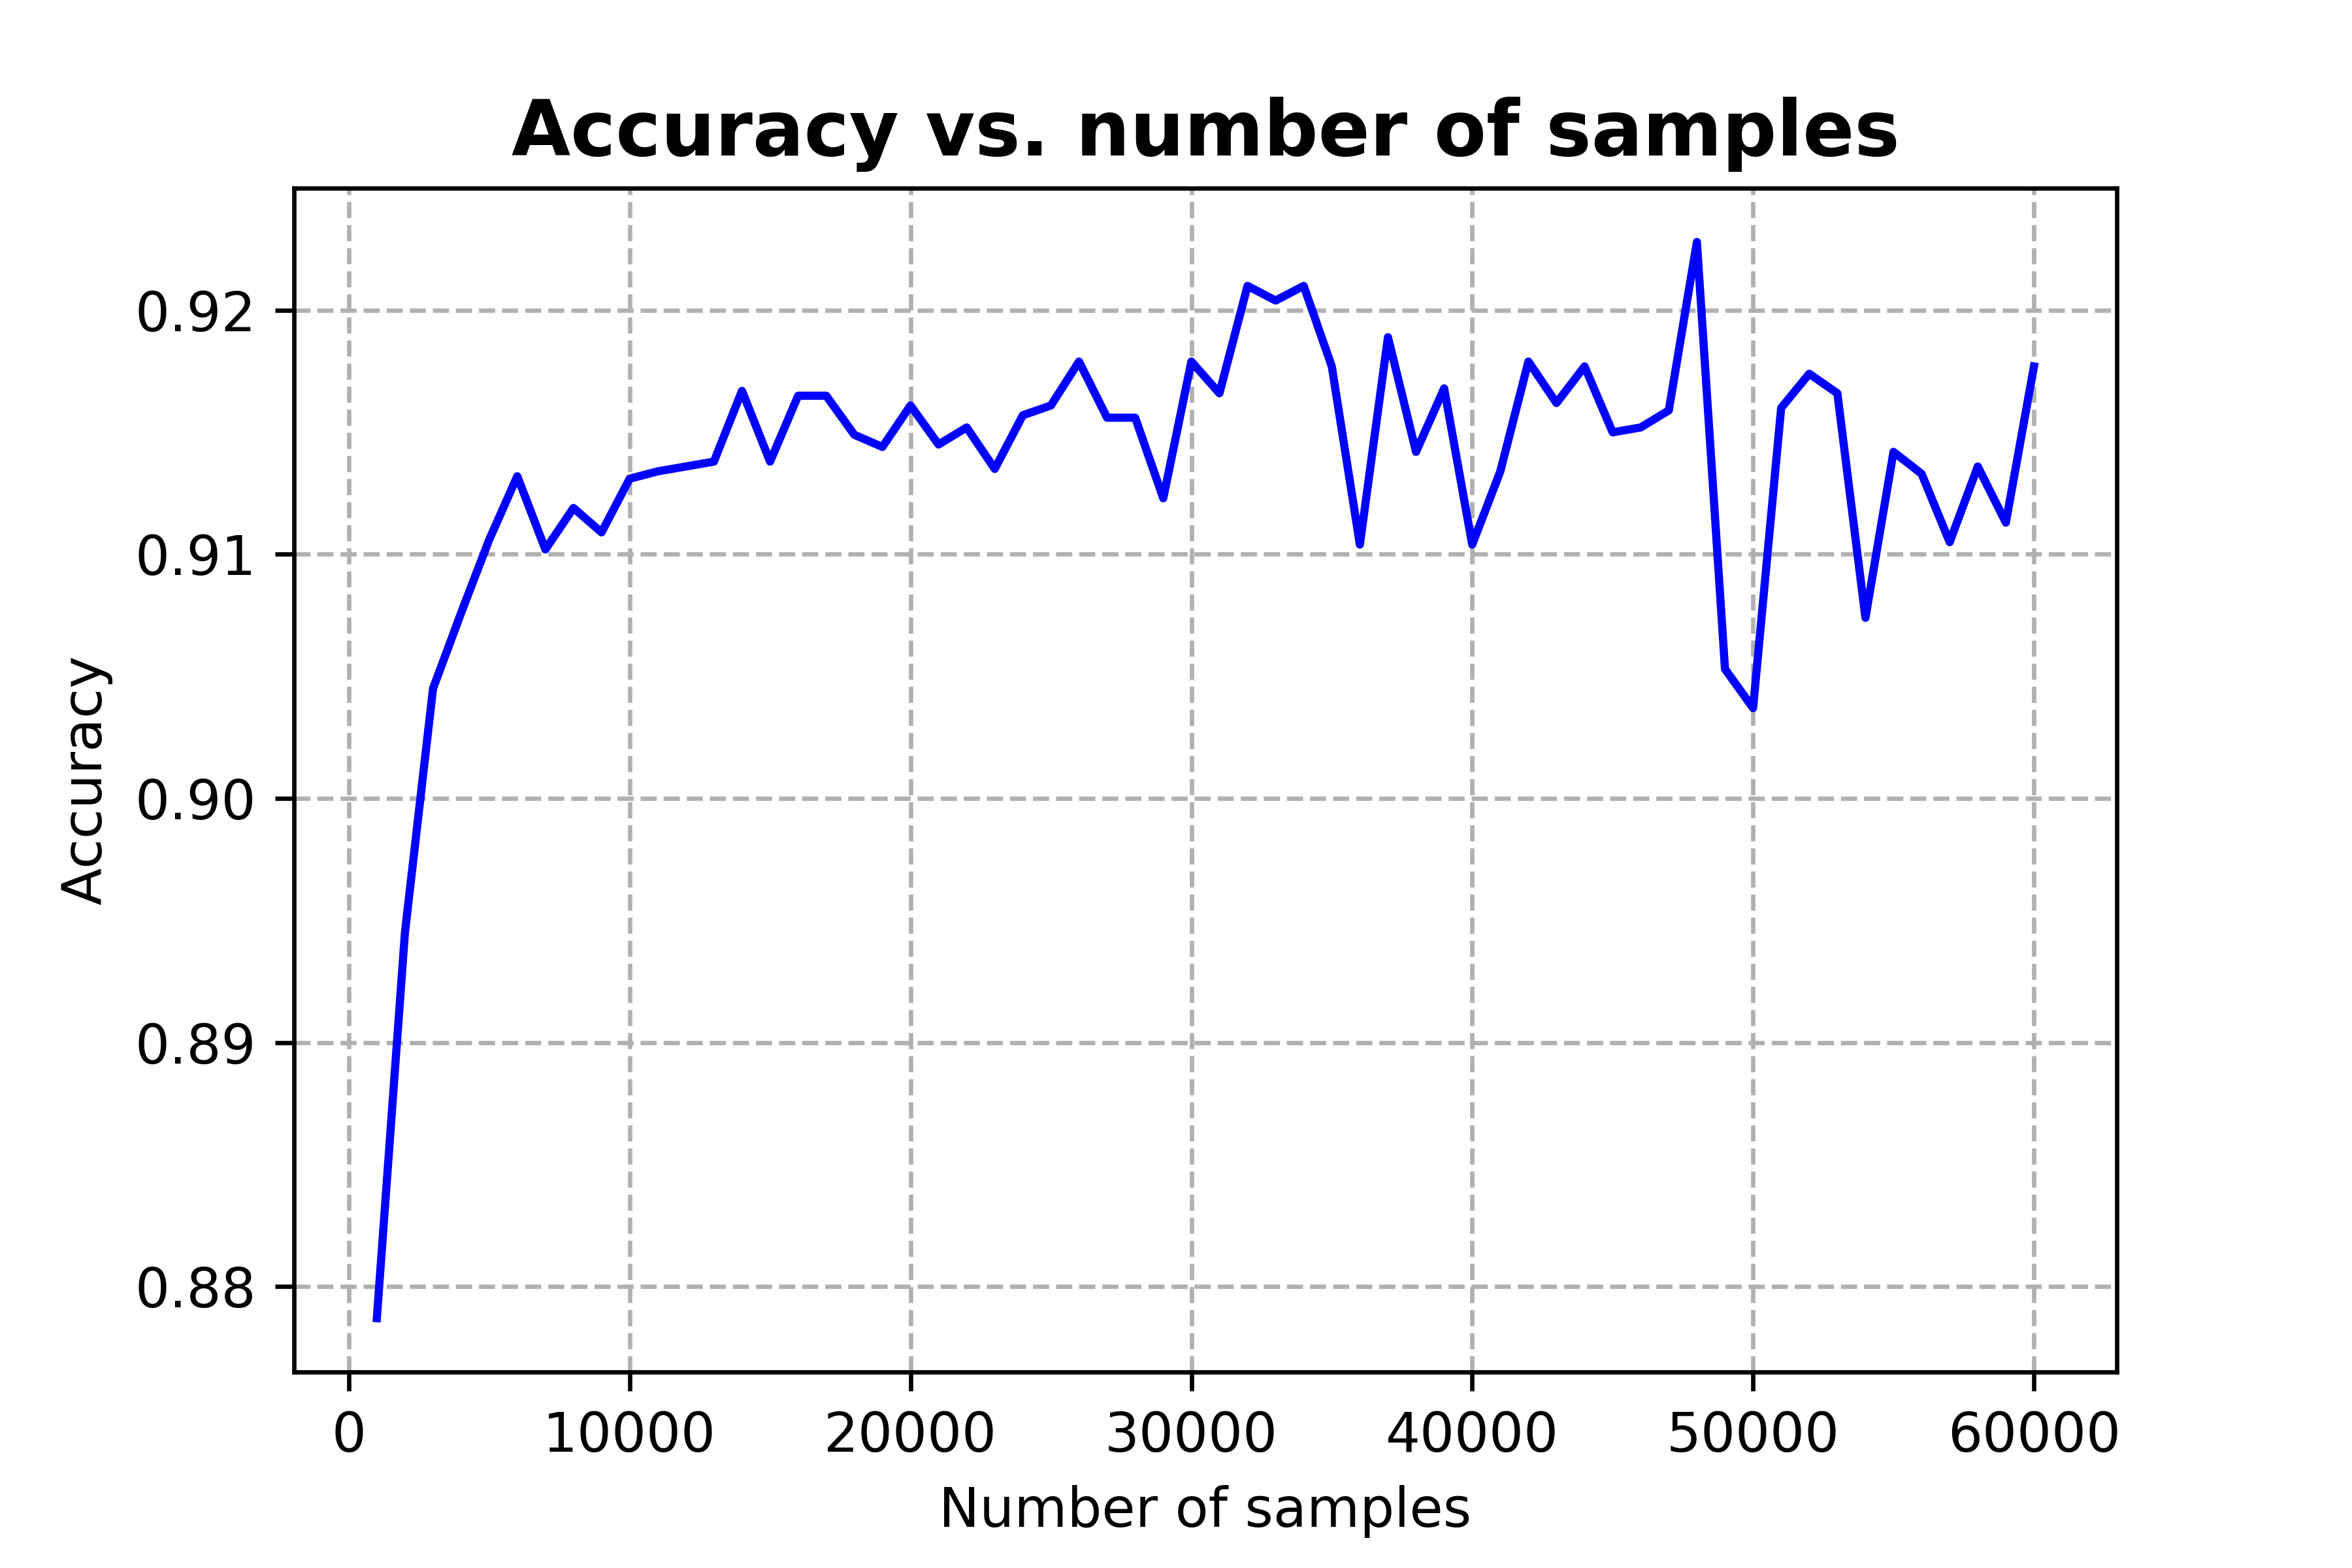
\includegraphics[width=1\linewidth]{figures/accuracy_vs_samples_linearsvm_default.png}
		\caption{SVM}\label{fig:1a}		
	\end{subfigure}
	\begin{subfigure}{0.35\linewidth}
		\centering
		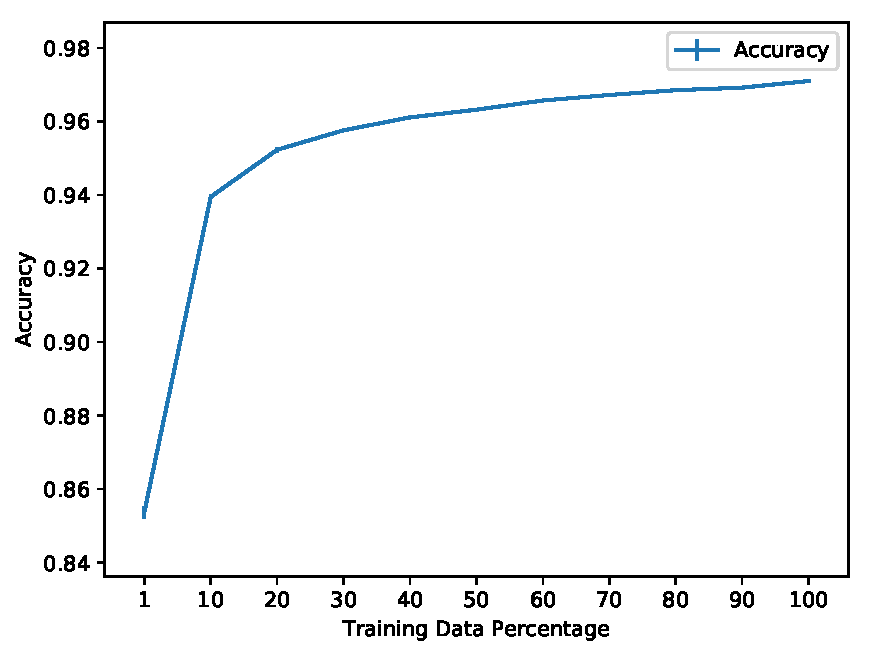
\includegraphics[width=1\linewidth]{figures/KNN_accuracy_vs_tss_with_fixed_k.pdf}
		\caption{KNN}\label{fig:1b}
	\end{subfigure}
	\begin{subfigure}{0.4\linewidth}
		\centering
		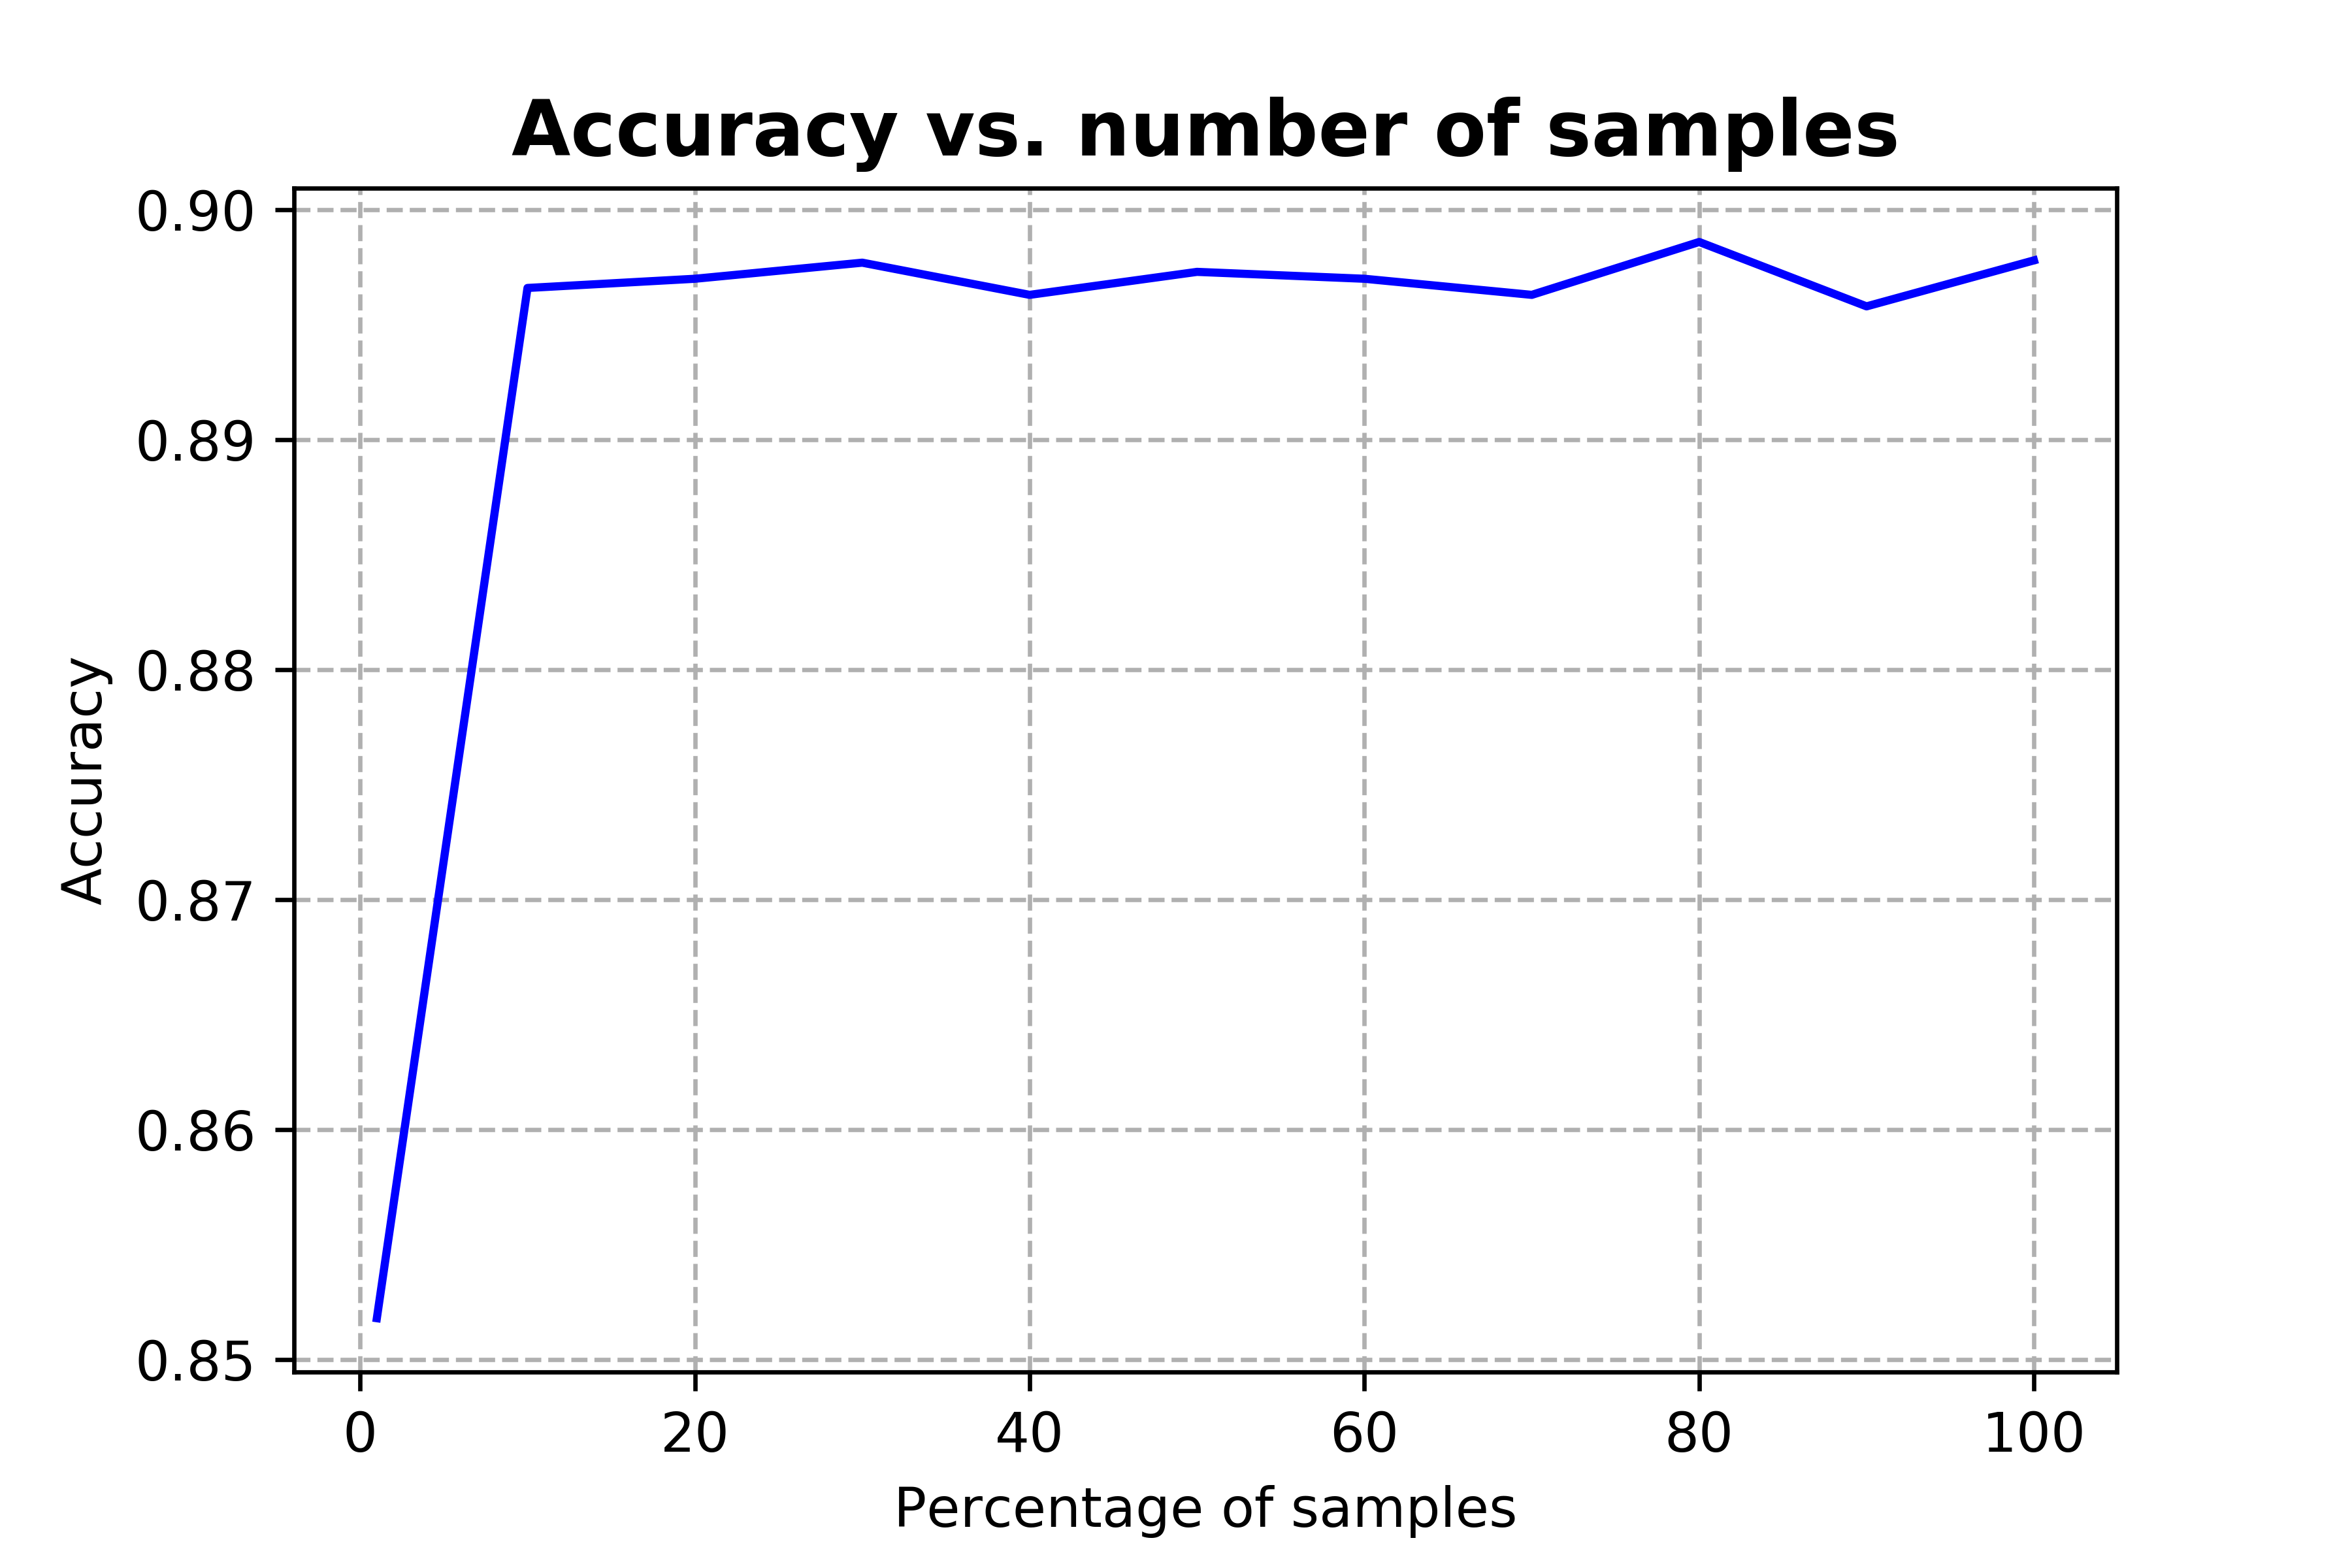
\includegraphics[width=1\linewidth]{figures/accuracy_vs_samples_neural_net_tuned.png}
		\caption{Neural Network}\label{fig:1b}
	\end{subfigure}
	\caption{Training set size vs. accuracy}\label{fig:1}
\end{figure}

\addcontentsline{toc}{subsection}{PCA features}
\subsection*{PCA features}
For this experiment, we computed the top-K principal component features such that the top-K principal components explained 90\% of the variance in the data. 
The results is shown in Figure \ref{fig:pca_features}.

From the plot we can see that the number PCA features are 87 out of 784 features which explains 90\% variance in the data.
\begin{figure}[H]
\centering
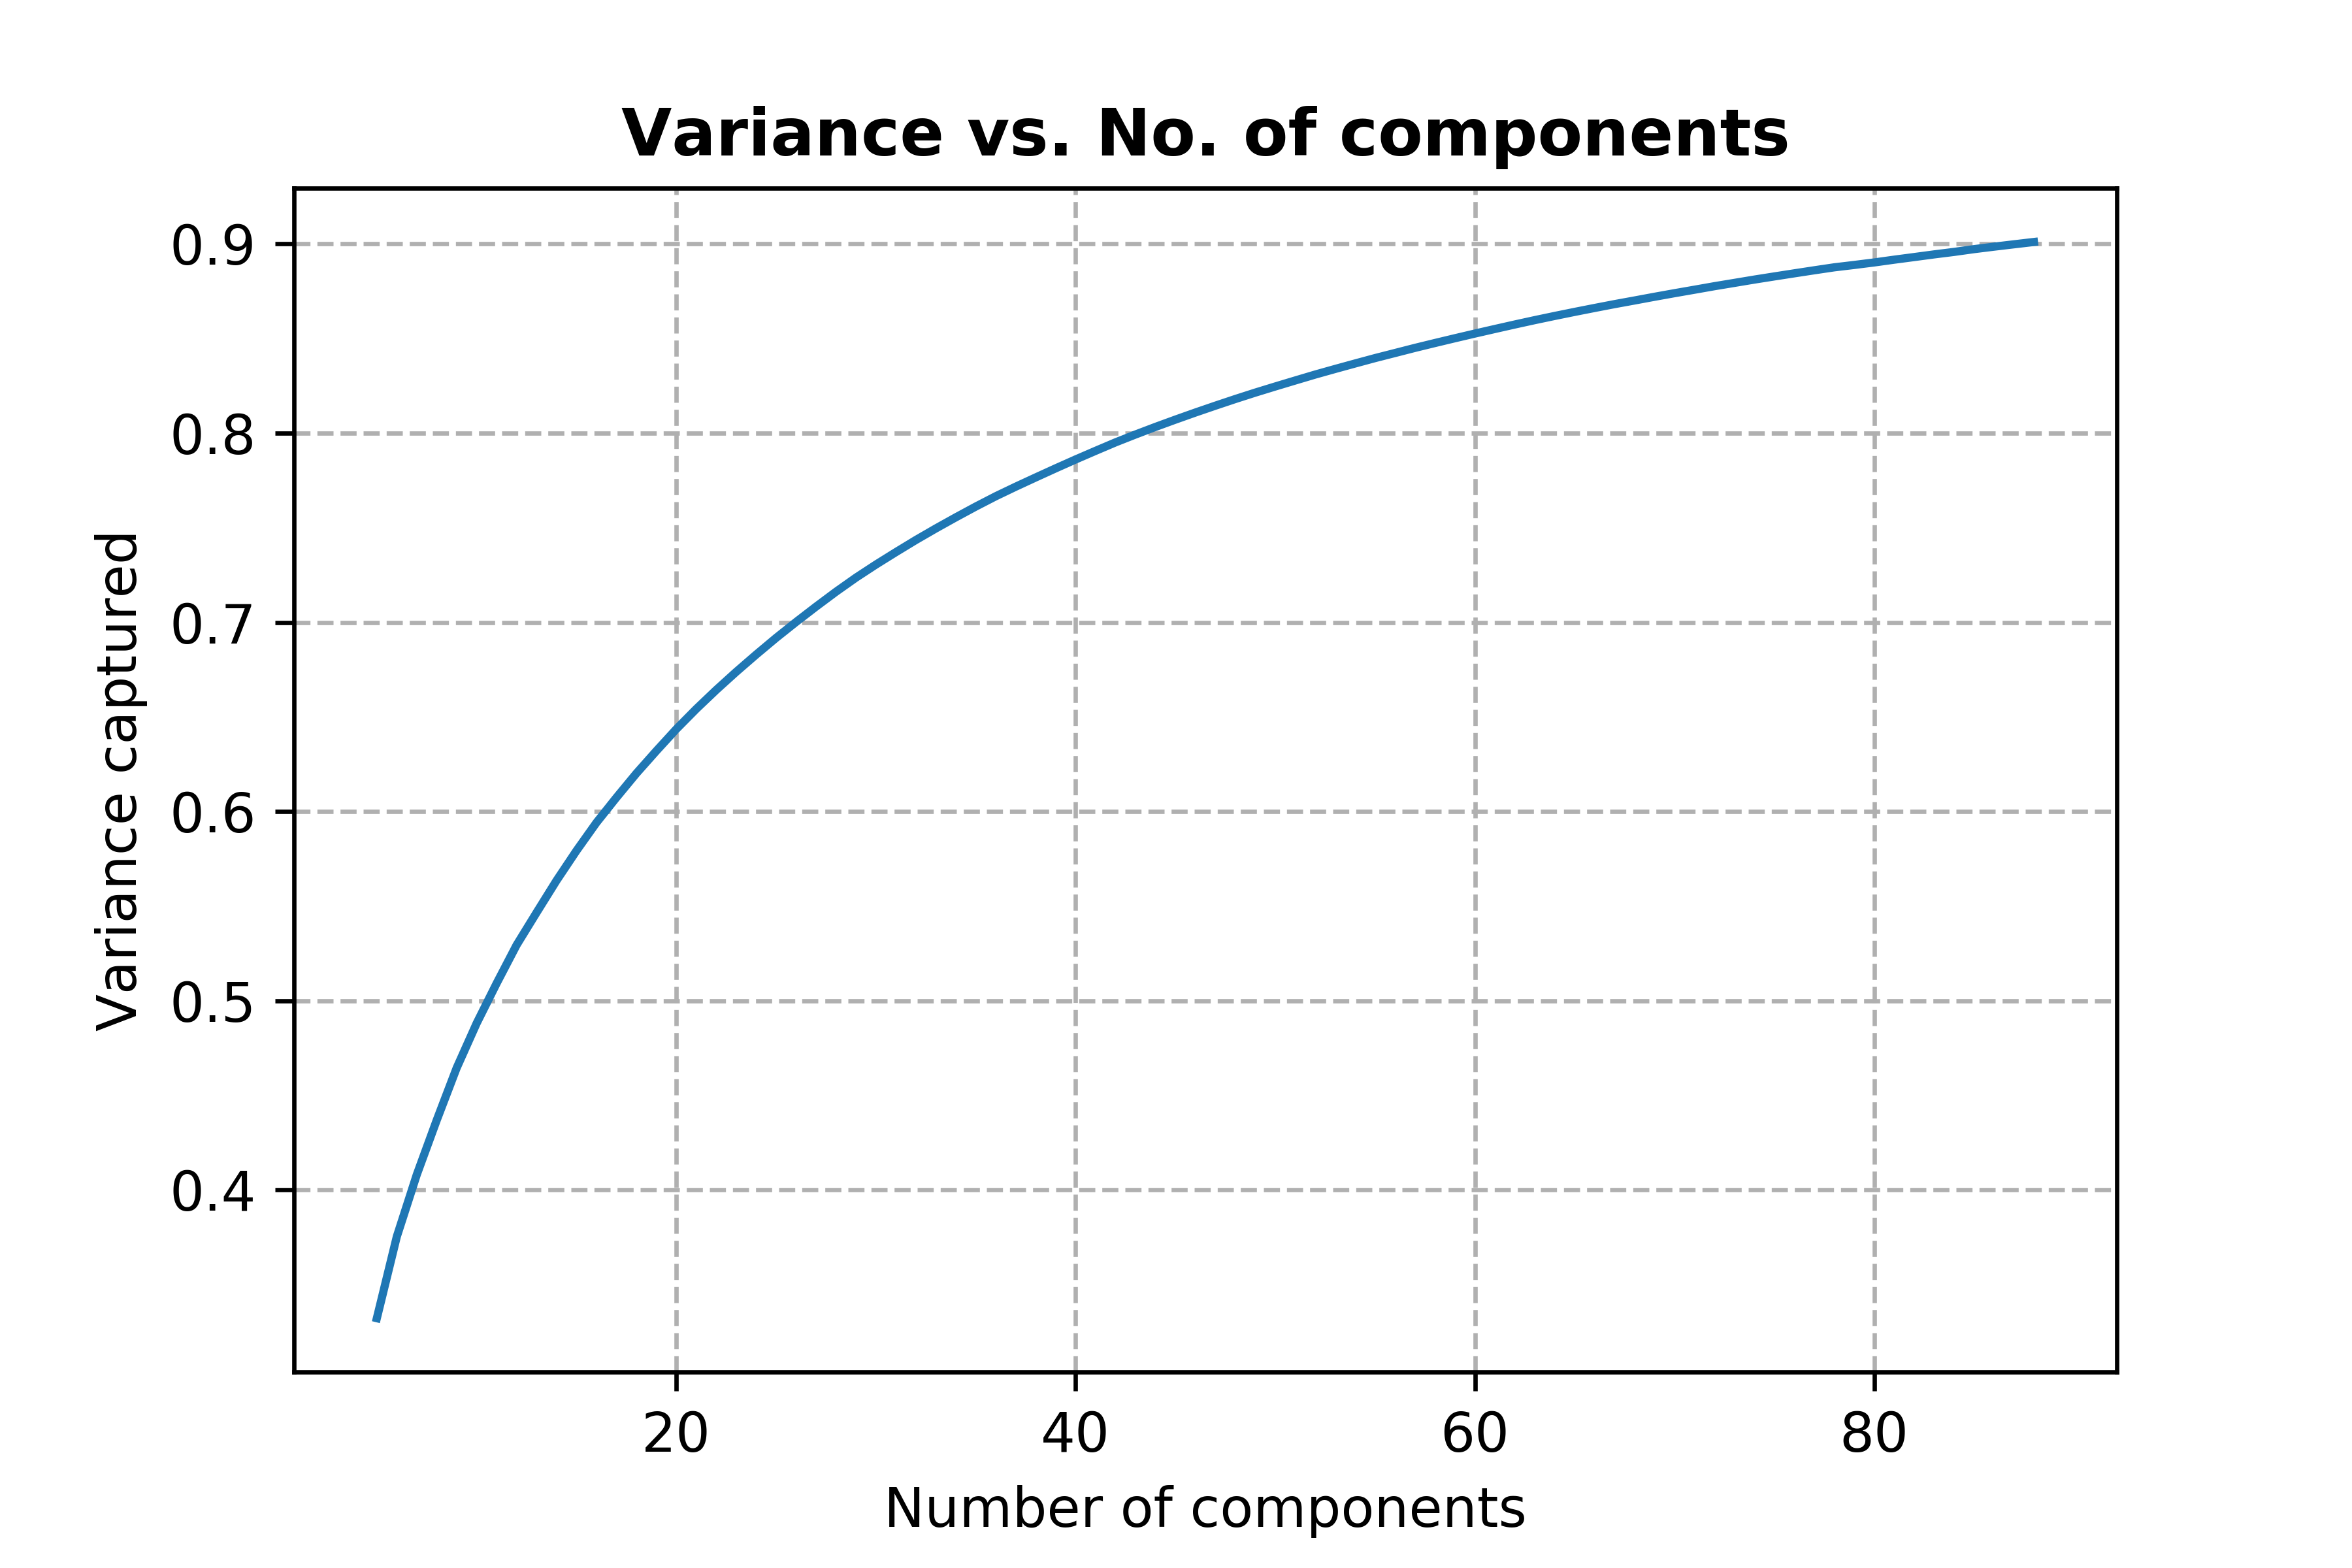
\includegraphics[width=0.5\linewidth]{figures/pca_variance_vs_no_comp.png}
\caption{PCA features. \label{fig:pca_features}}
\end{figure}

\addcontentsline{toc}{subsection}{Hypothesis testing}
\subsection*{Hypothesis testing}

The following sections contain the results of the hypothesis testing under various conditions and for different combinations. The results shown are basically the rejection or the acceptance of the null hypothesis (accepting $\mu_{1} = \mu_{2}$) when comparing between different algorithms under different settings.

The parameters that have been used for each algorithm are the values that were found during the parameter tuning stage of the project. So, for all of these experiments, the parameter setting remain the same and the difference is mostly in the pre-processing of the data (performing PCA or not performing PCA). The aim of this was to study was two-fold:

\begin{itemize}
\item To understand the effect of performing PCA on the data and to see if the results are consistent with using the actual data. This should help us in reducing the training time overall since the PCA data would have low dimensionality. 

\item To compare the algorithms that were used to classify the dataset.
\end{itemize}


\addcontentsline{toc}{subsubsection}{Comparison using PCA data}
\subsubsection*{Comparison using PCA data}

Here, all the results shown are experiments that were run using PCA data. The way in which the PCA data is being generated was described in a previous section and this method ensures that we don't use any information from the test data for training.

\begin{table}[H]
\centering
\begin{tabular}{ c|c|c } 
 \textbf{Experiment} & \textbf{Result} & \textbf{Inference} \\ 
 \hline
Neural Net vs. SVM & $x > x_{\alpha}$ & Neural Net ($\mu_{NN} > \mu_{SVM}$) Reject Null Hypothesis\\ 
KNN vs. SVM & $x > x_{\alpha}$ &  KNN ($\mu_{KNN} > \mu_{SVM}$) Reject Null Hypothesis\\ 
KNN vs. Neural Net & $x > x_{\alpha}$ &  KNN ($\mu_{KNN} > \mu_{NN}$) Reject Null Hypothesis \\
\end{tabular}
\caption{Hypothesis testing results (with PCA) \label{tab:hypo_test_pca}}
\end{table}

\paragraph{Observations.}
\begin{itemize}
\item{\textbf{Support Vector Machine.}} The results of the hypothesis testing test run for SVM is shown in Figs. \ref{fig:acc_svm_hypo_pca} and \ref{fig:hypo_pca_svm_roc_conf}. The first figure shows the accuracy variation over the 10-folds of CV experiment. The second figure shows the confusion matrix and ROC curve for the run for the $1^{st}$ fold. 

These can be thought of to represent the best run of the algorithm since we use the optimized parameters. To get better perspectives of the experiment, the precision and recall curves have also been included in Fig. \ref{fig:hypo_pca_svm_pre_recl}.

\begin{figure}[H]
\centering
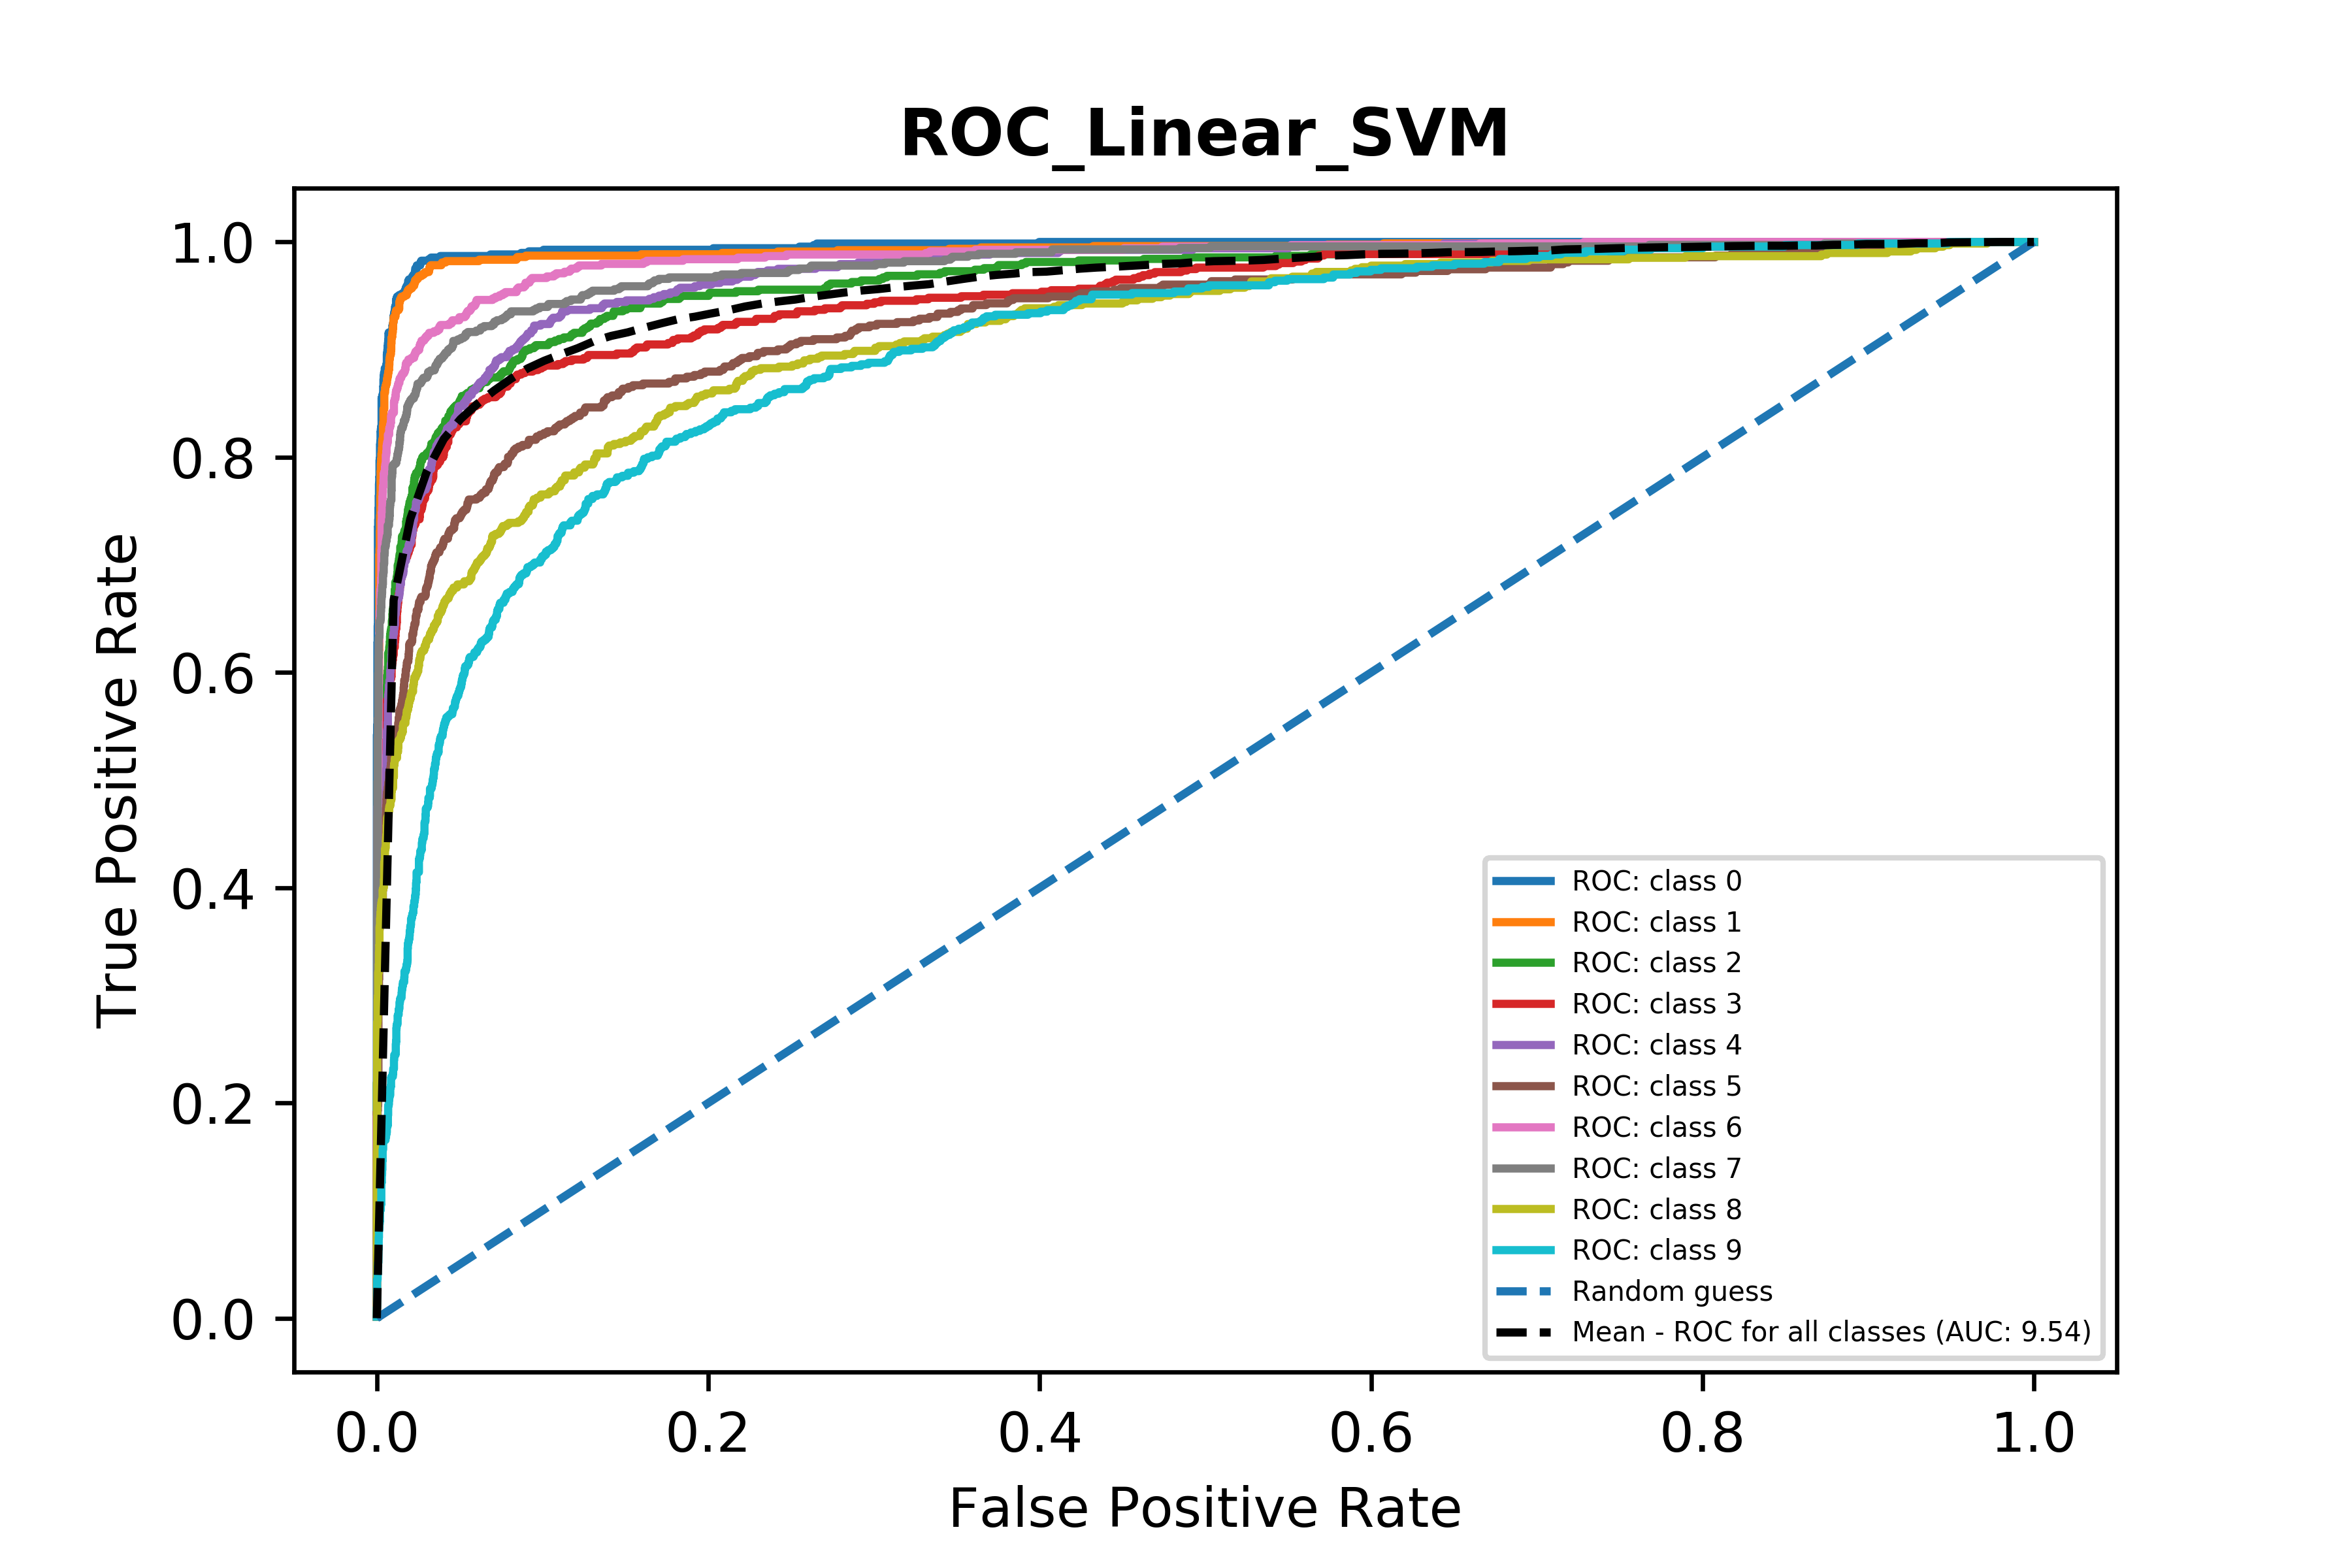
\includegraphics[width=0.45\linewidth]{figures/SVM_linear_ROC_C_70_k_1_using_pca.png} 
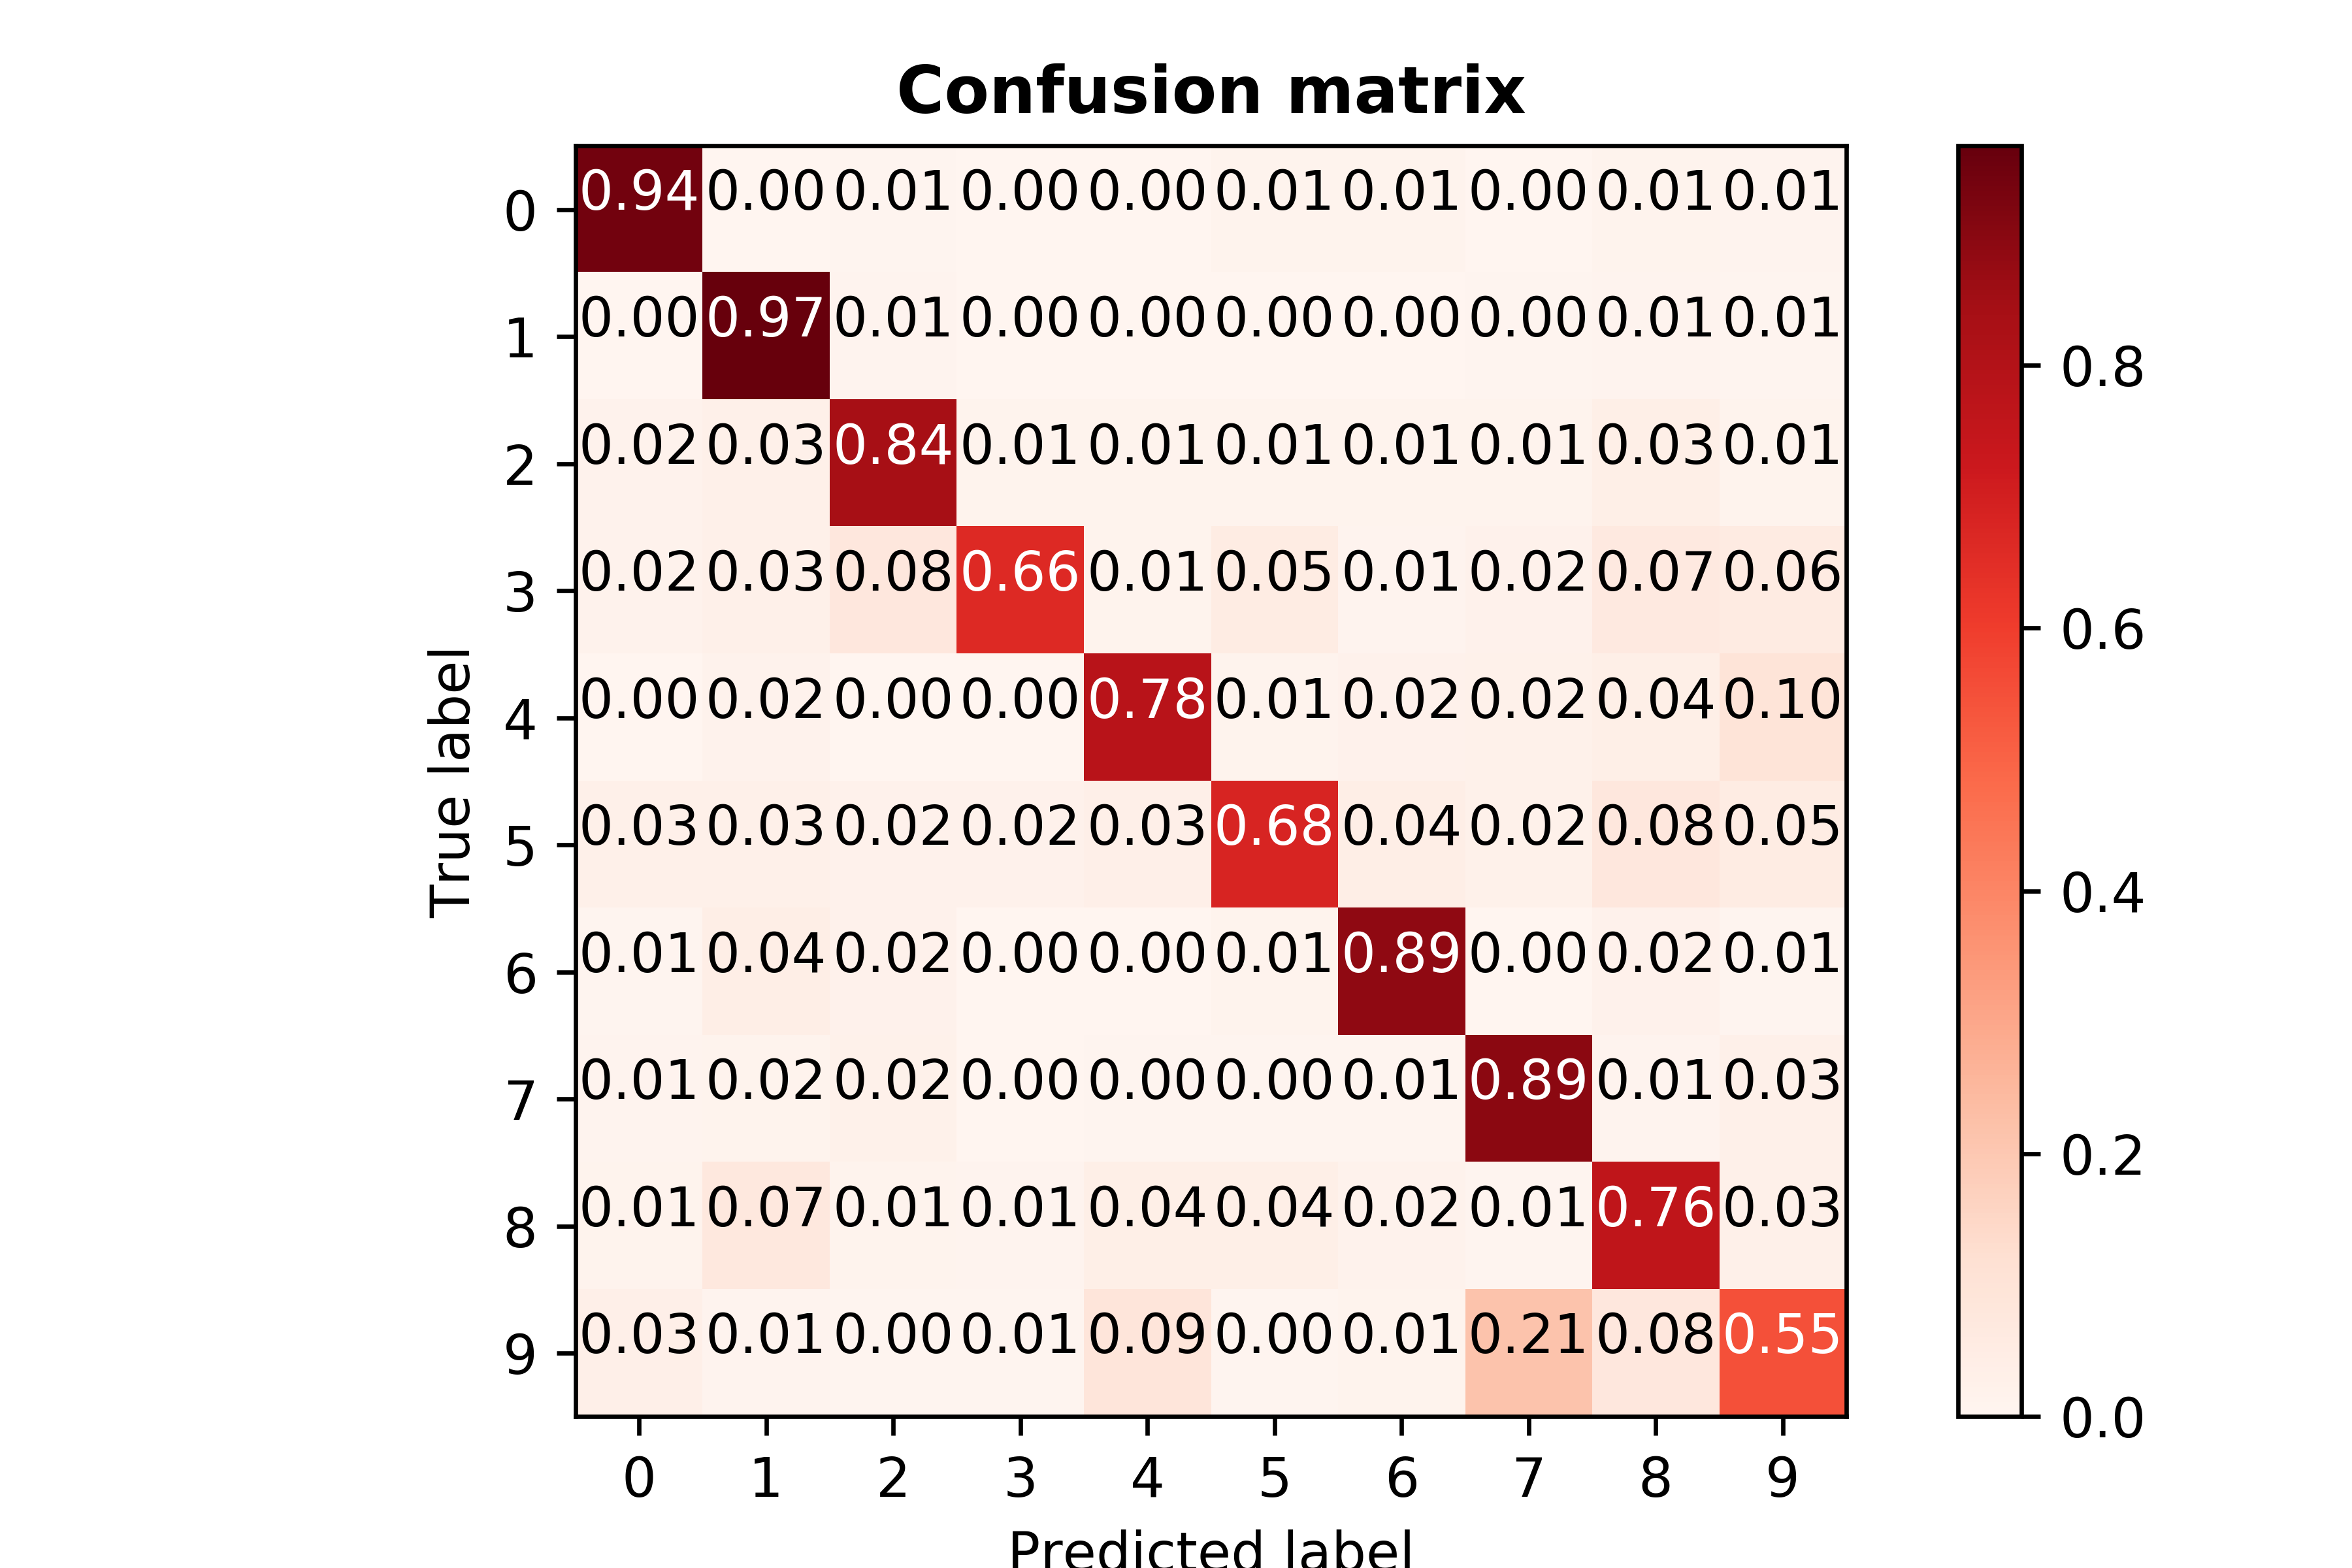
\includegraphics[width=0.5\linewidth]{figures/SVM_Conf_matrix_C_70_k_1_using_pca.png}
\caption{(Left) ROC curve. (Right) Confusion matrix [Hypothesis test SVM with PCA] \label{fig:hypo_pca_svm_roc_conf}}
\end{figure}

\begin{figure}[H]
\centering
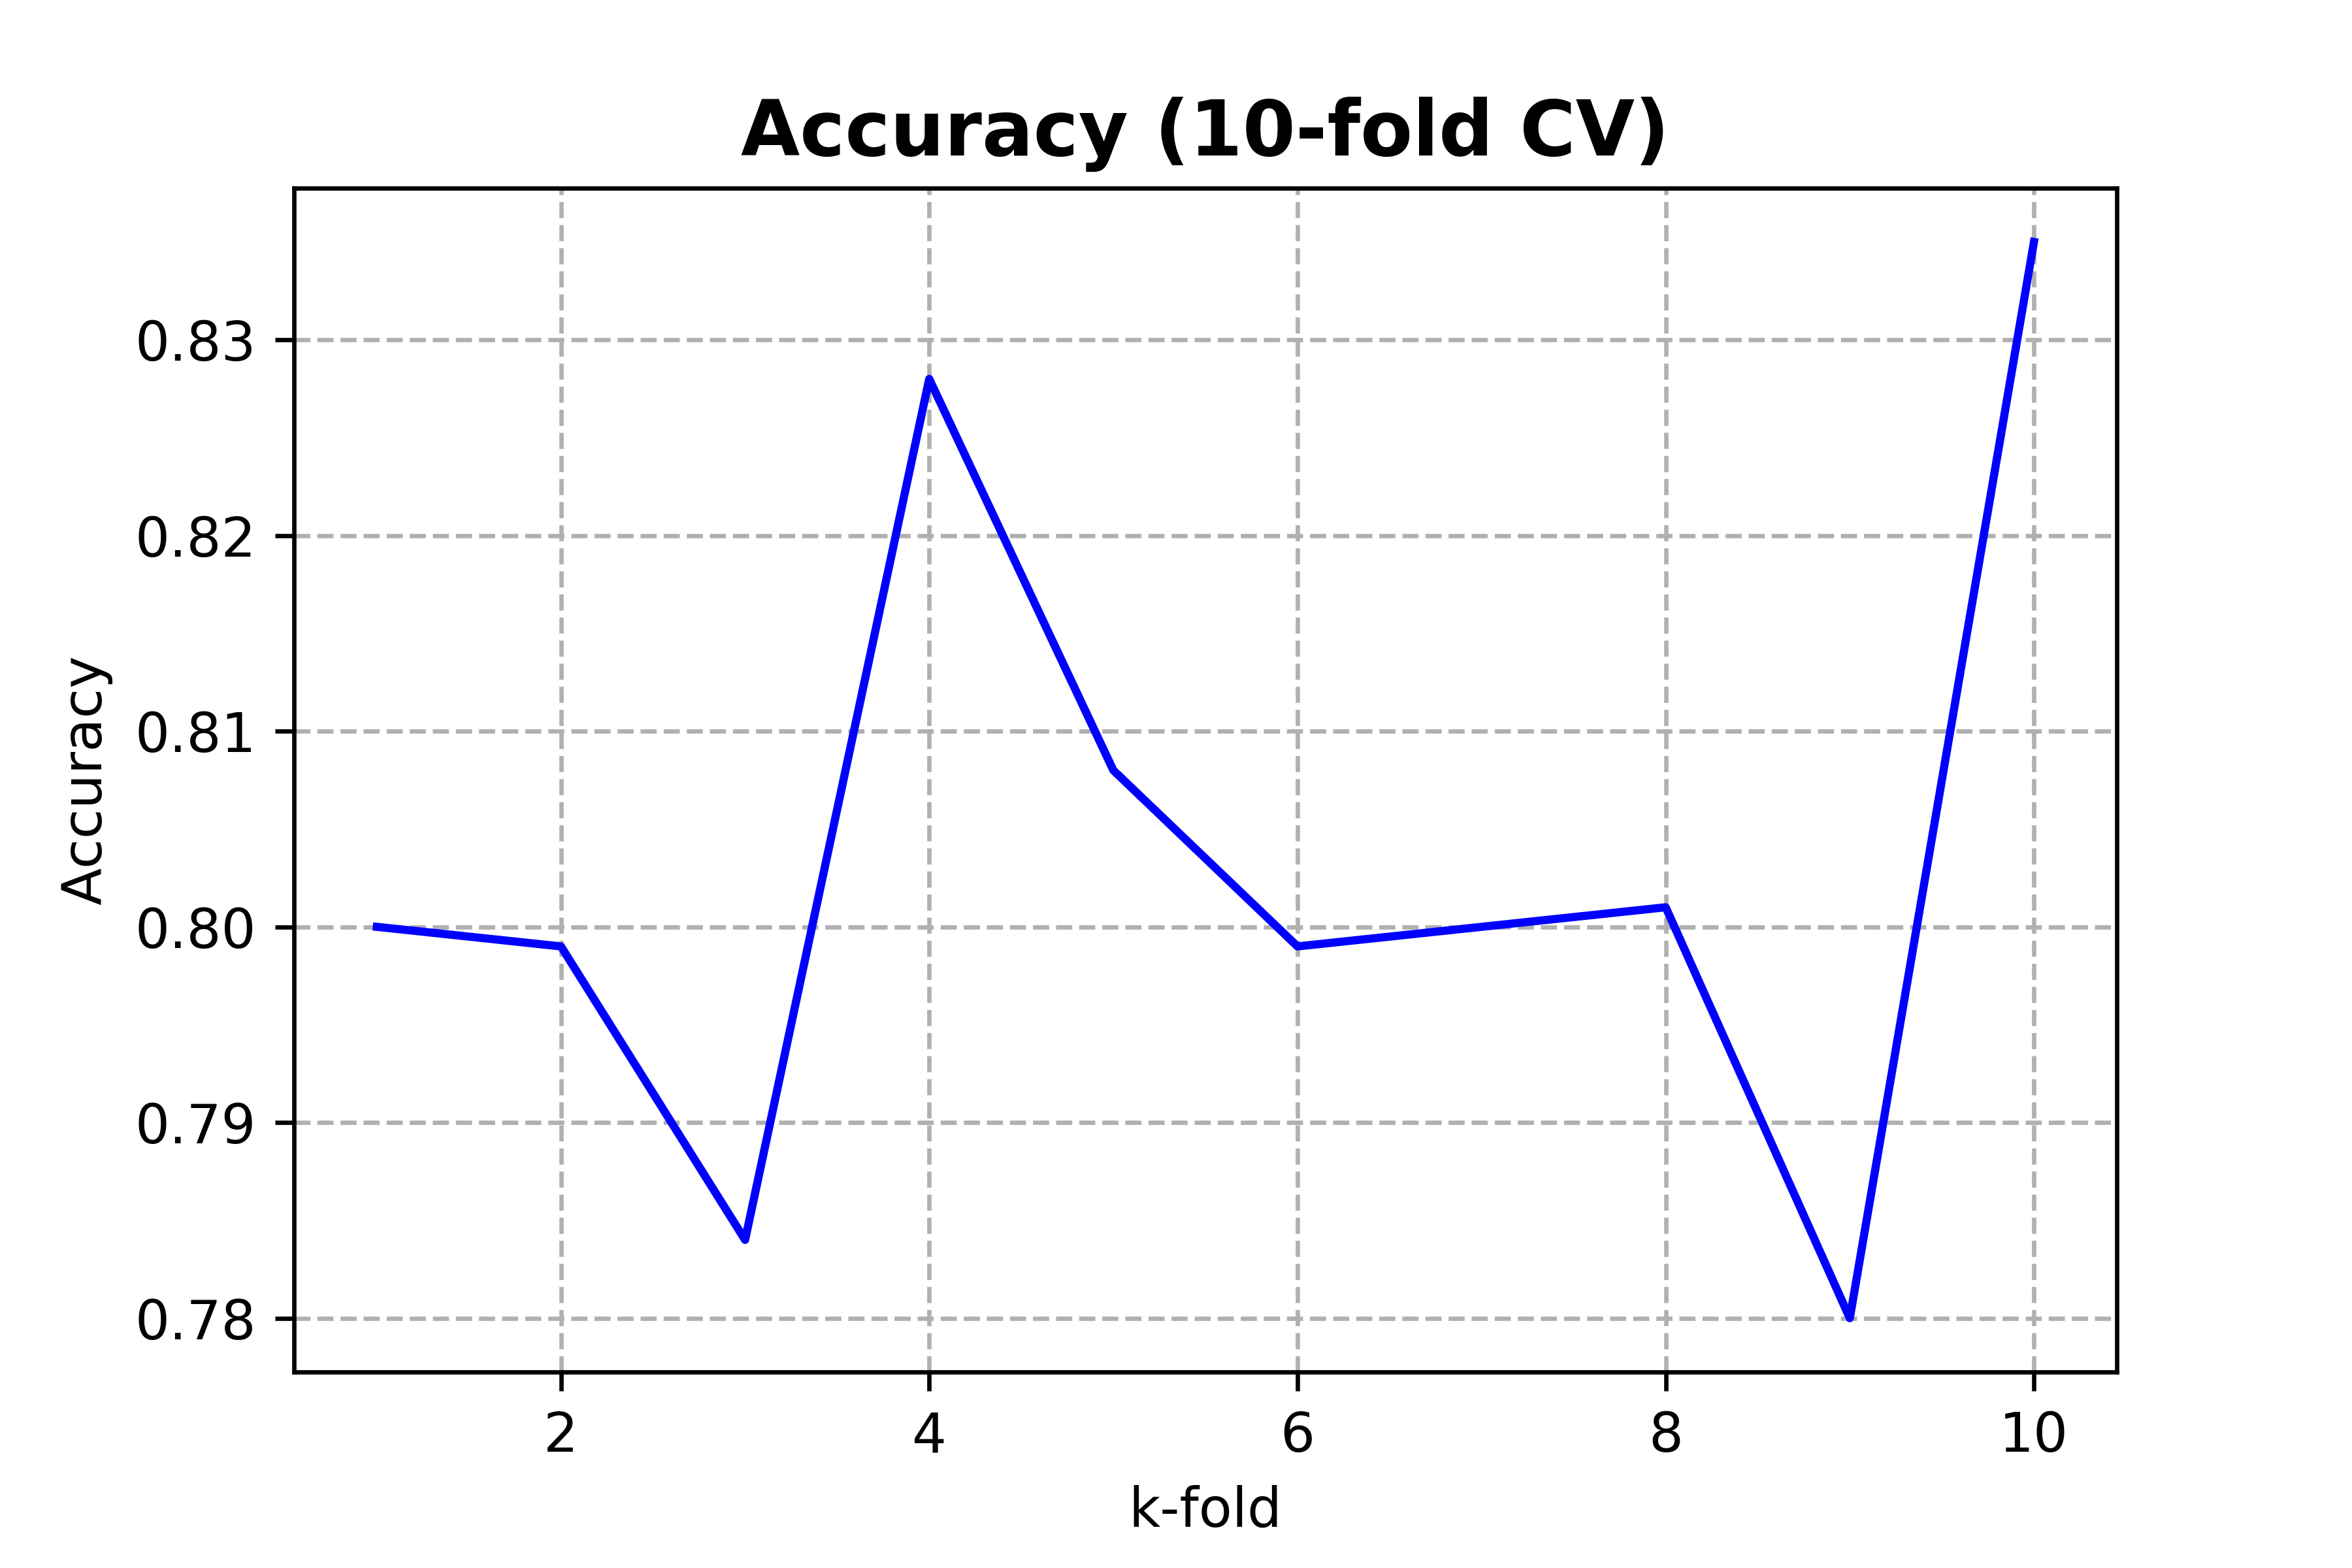
\includegraphics[width=0.5\linewidth]{figures/acc_svm_tuned_pca_hypo.png}
\caption{Accurcay (SVM) over the 10-fold CV (Hypothesis testing - with PCA). \label{fig:acc_svm_hypo_pca}}
\end{figure}

\begin{figure}[H]
\centering
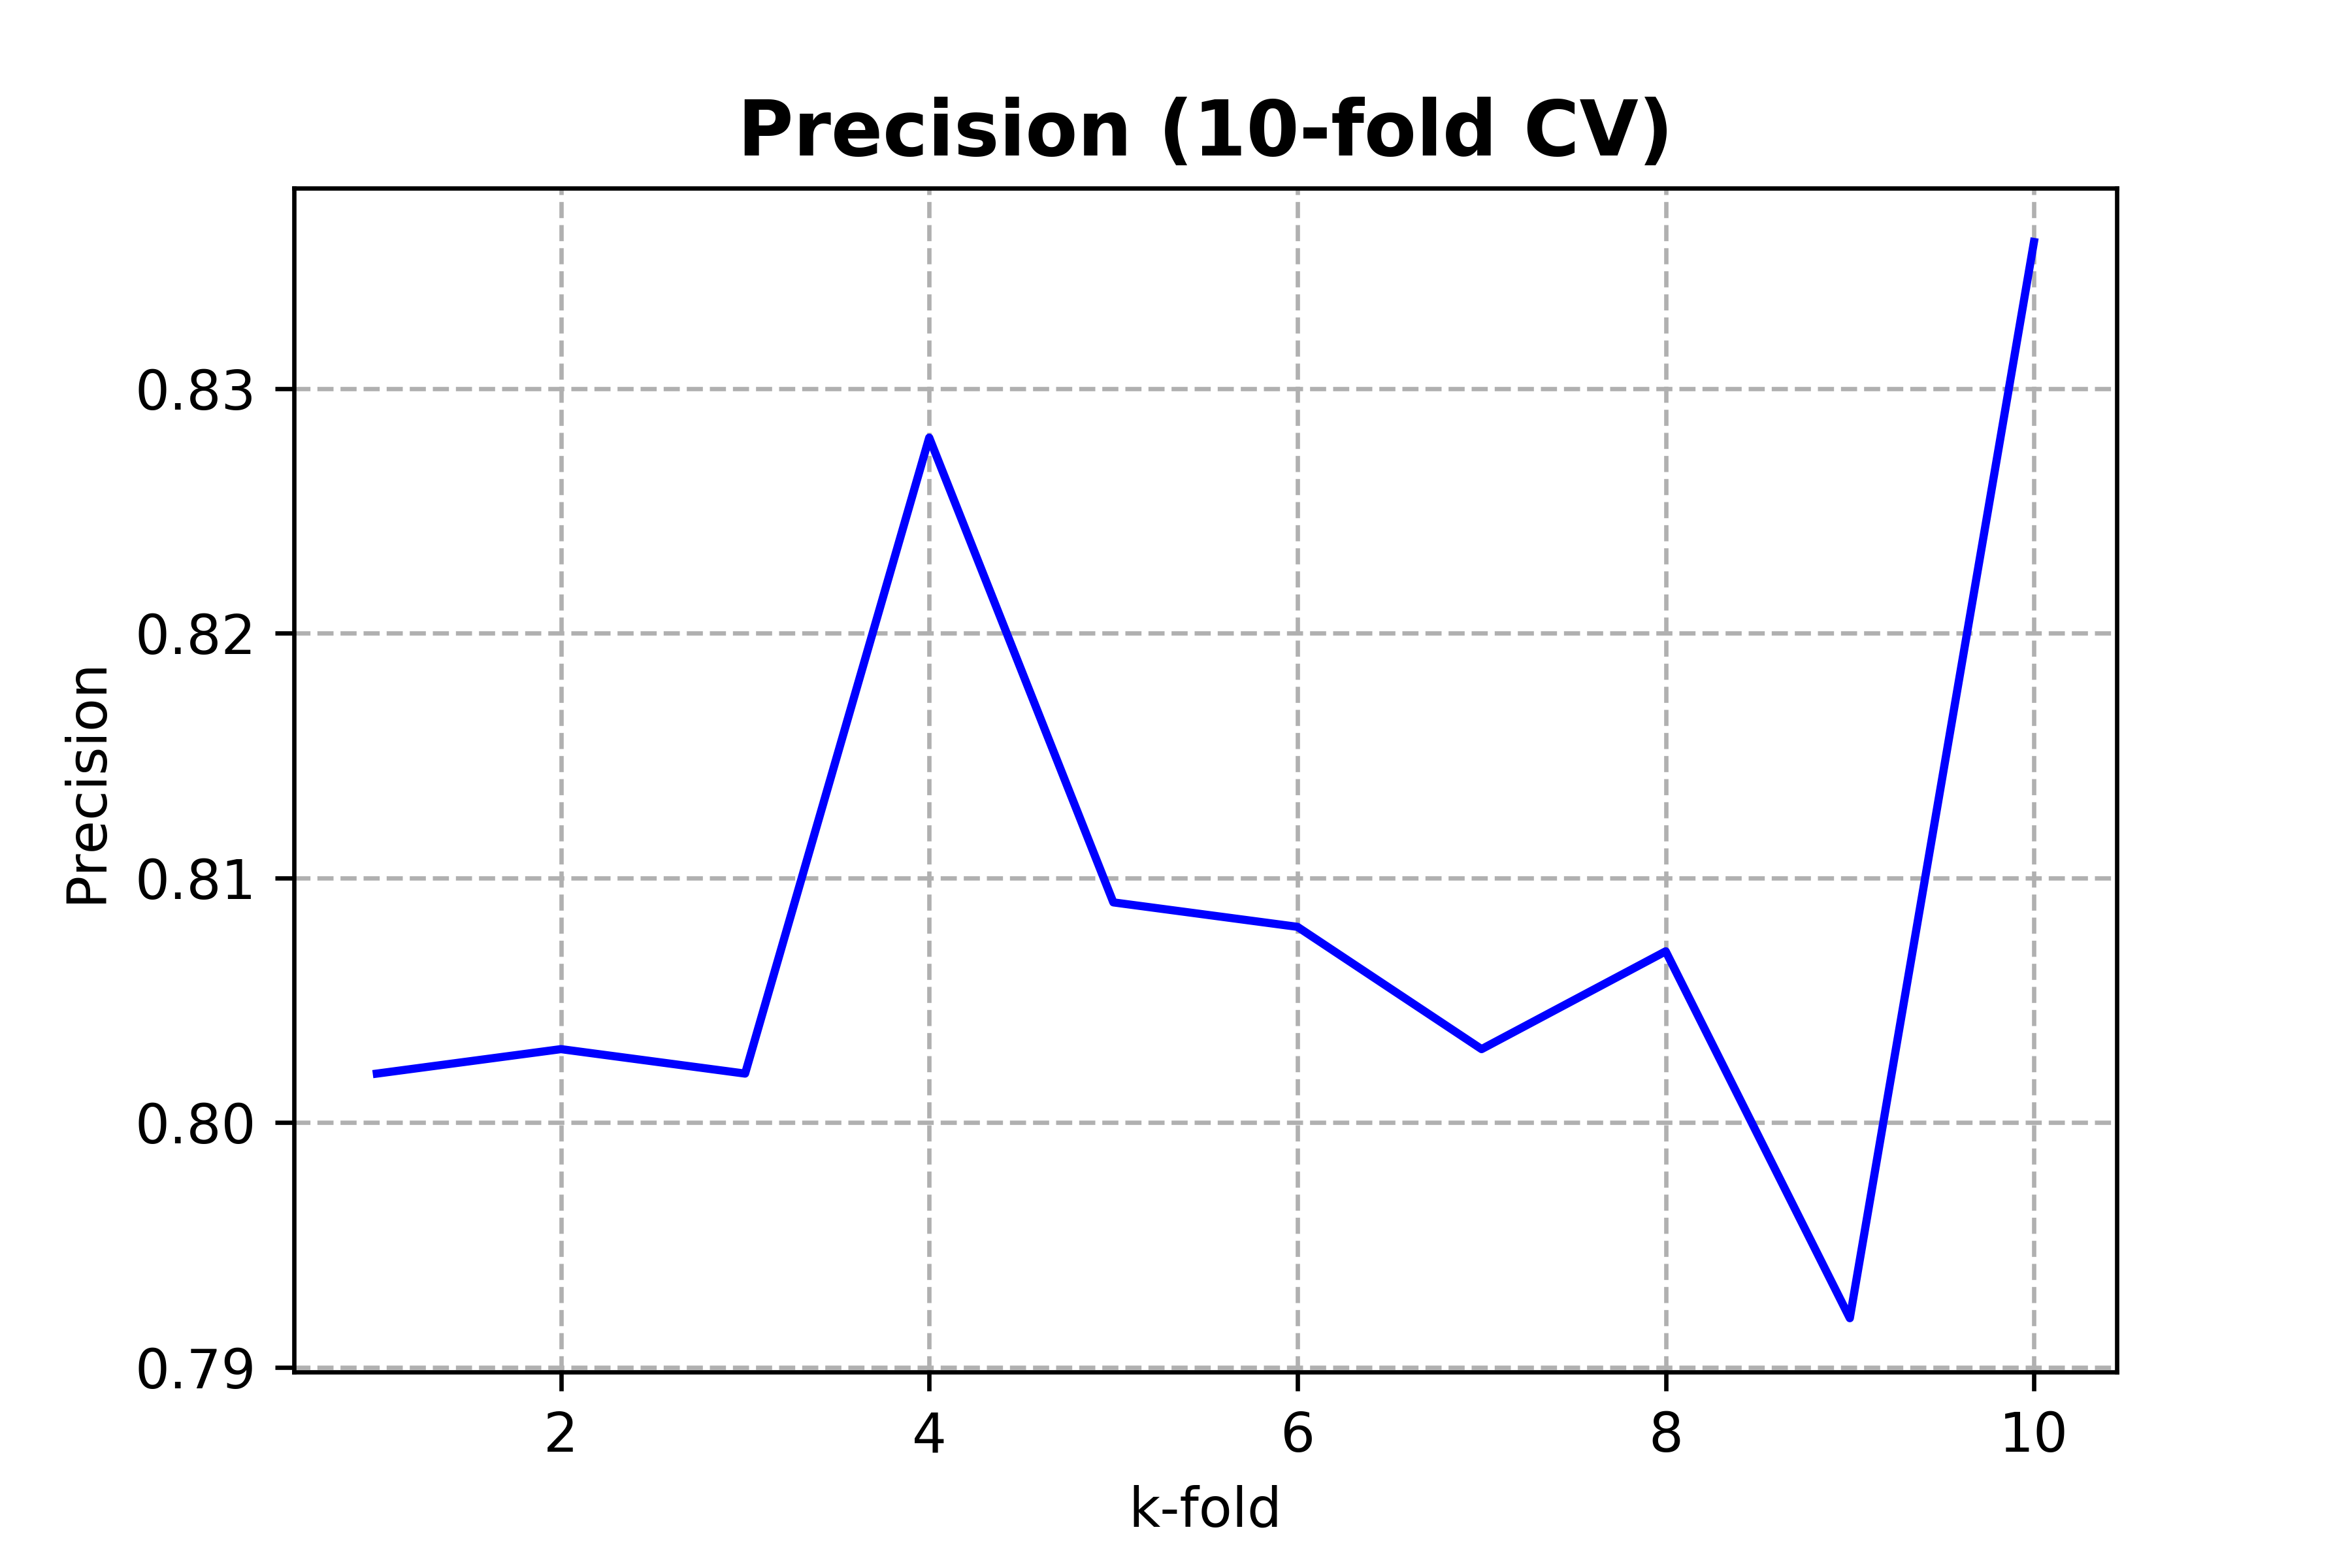
\includegraphics[width=0.45\linewidth]{figures/precision_svm_tuned.png} 
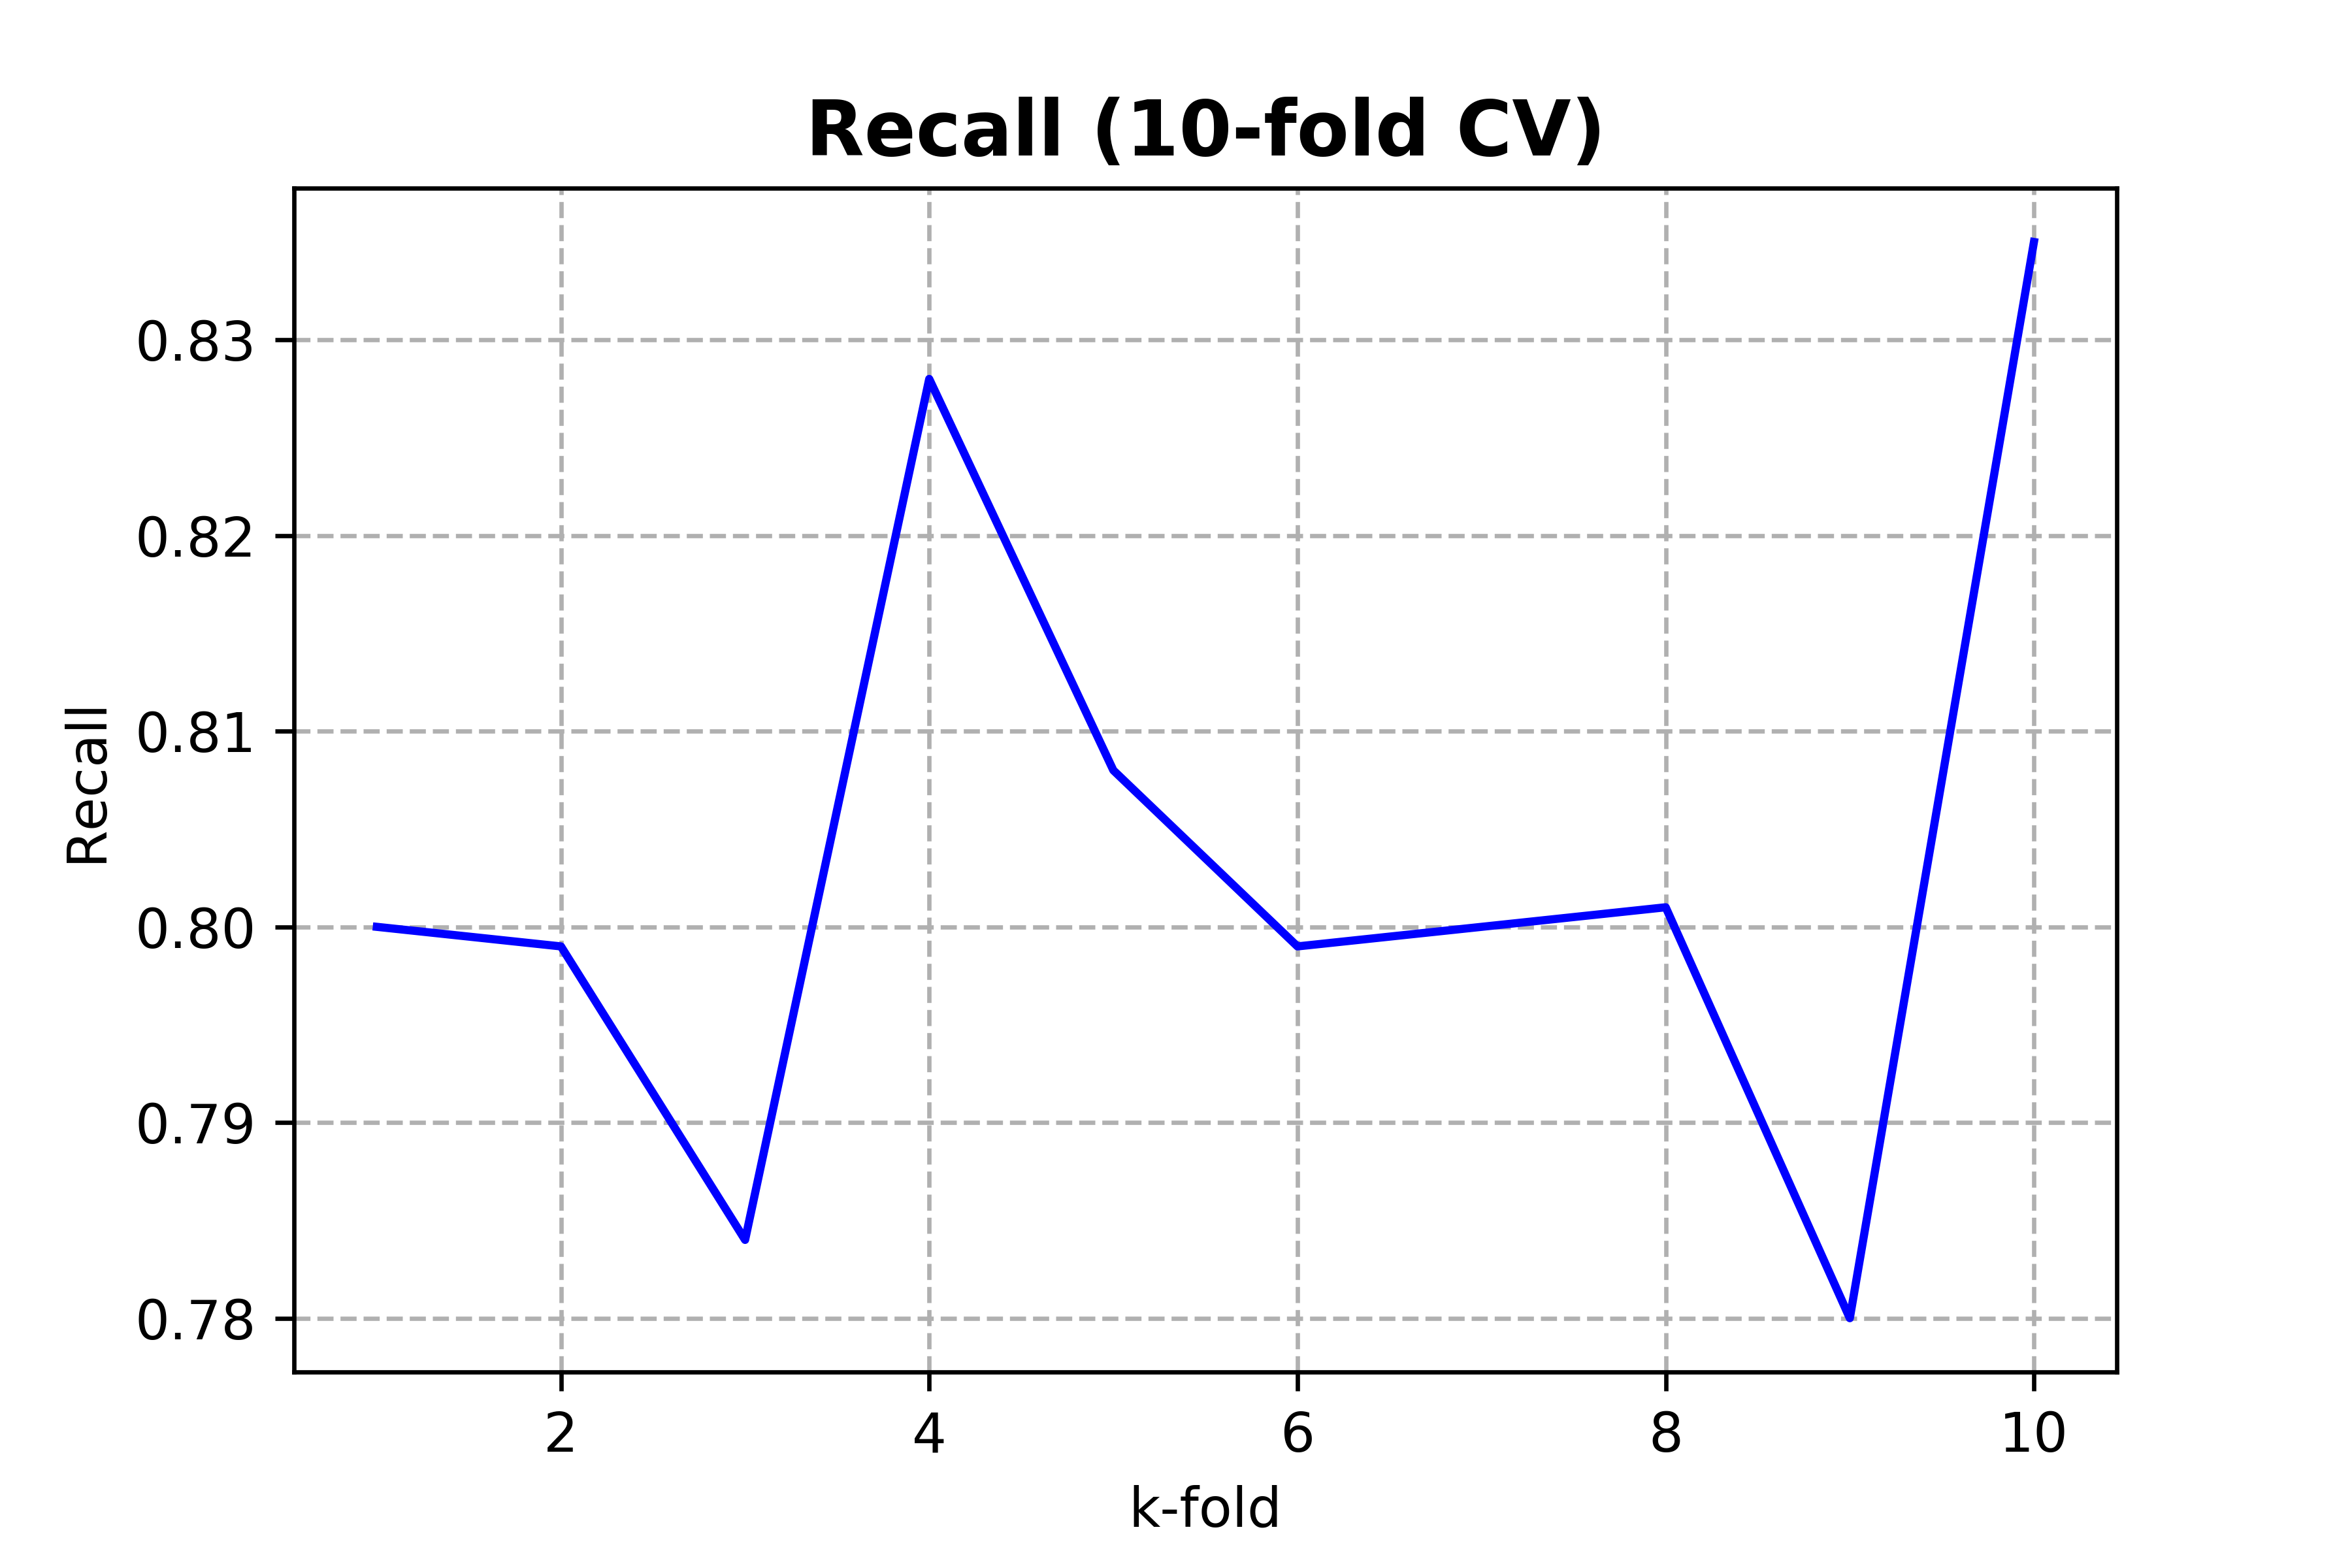
\includegraphics[width=0.45\linewidth]{figures/recall_svm_tuned.png}
\caption{(Left) Precision curve. (Right) Recall curve. [Hypothesis test SVM with PCA] \label{fig:hypo_pca_svm_pre_recl}}
\end{figure}

\item{\textbf{Neural Network.}} The results for the Hypothesis run for Neural Network is shown in Figs \ref{fig:acc_nn_hypo_pca}, \ref{fig:hypo_pca_nn_pre_recl} and \ref{fig:hypo_pca_nn_roc_conf}. The results can be compared to the SVM runs and it is obvious that the Neural Net performs better than the SVM from a look at the plots for both. This is reflected in the hypothesis result table \ref{tab:hypo_test_pca}.

\begin{figure}[H]
\centering
\includegraphics[width=0.45\linewidth]{figures/{Neural_Net_linear_ROC_Alpha_100_Act_fcn_logistic_Learn_rate_0.002_k_1_using_pca}.png} 
\includegraphics[width=0.5\linewidth]{figures/{Neural_Net_Conf_matrix_Alpha_100_Act_fcn_logistic_Learn_rate_0.002_k_1_using_pca}.png}
\caption{(Left) ROC curve. (Right) Confusion matrix [Hypothesis test NN with PCA] \label{fig:hypo_pca_nn_roc_conf}}
\end{figure}

\begin{figure}[H]
\centering
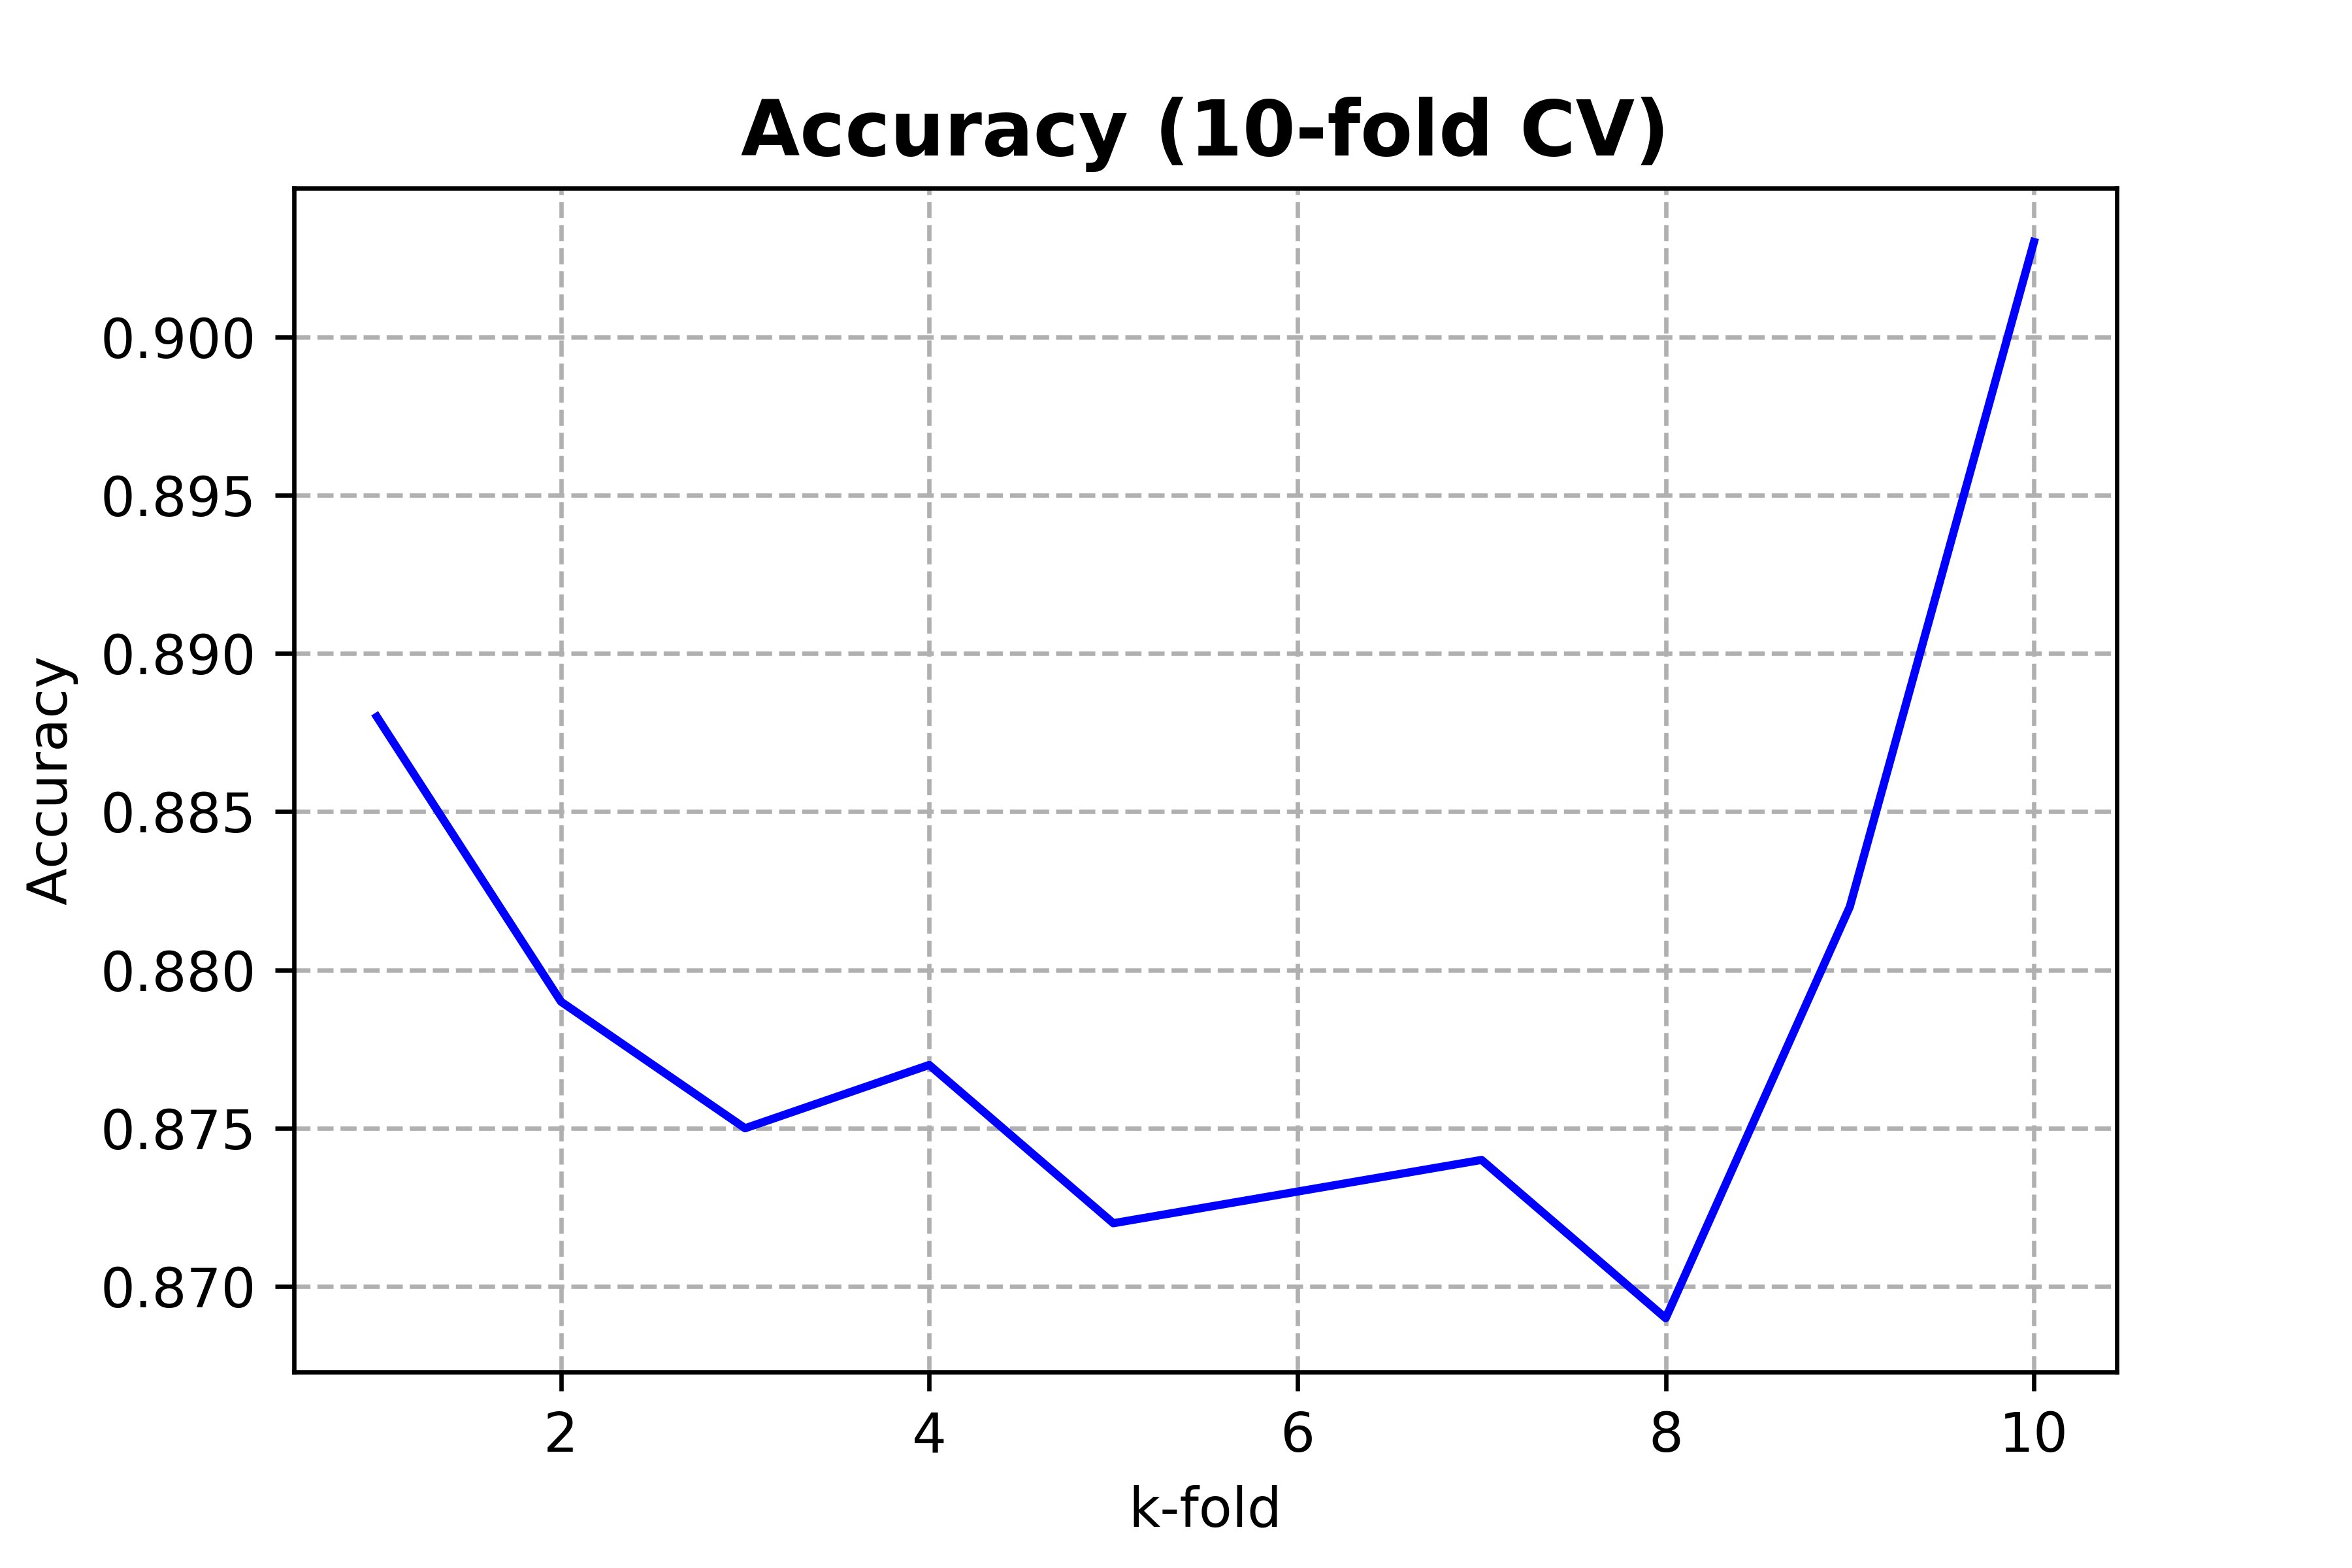
\includegraphics[width=0.5\linewidth]{figures/acc_nn_tuned_pca_hypo.png}
\caption{Accurcay (NN) over the 10-fold CV (Hypothesis testing - with PCA). \label{fig:acc_nn_hypo_pca}}
\end{figure}

\begin{figure}[H]
\centering
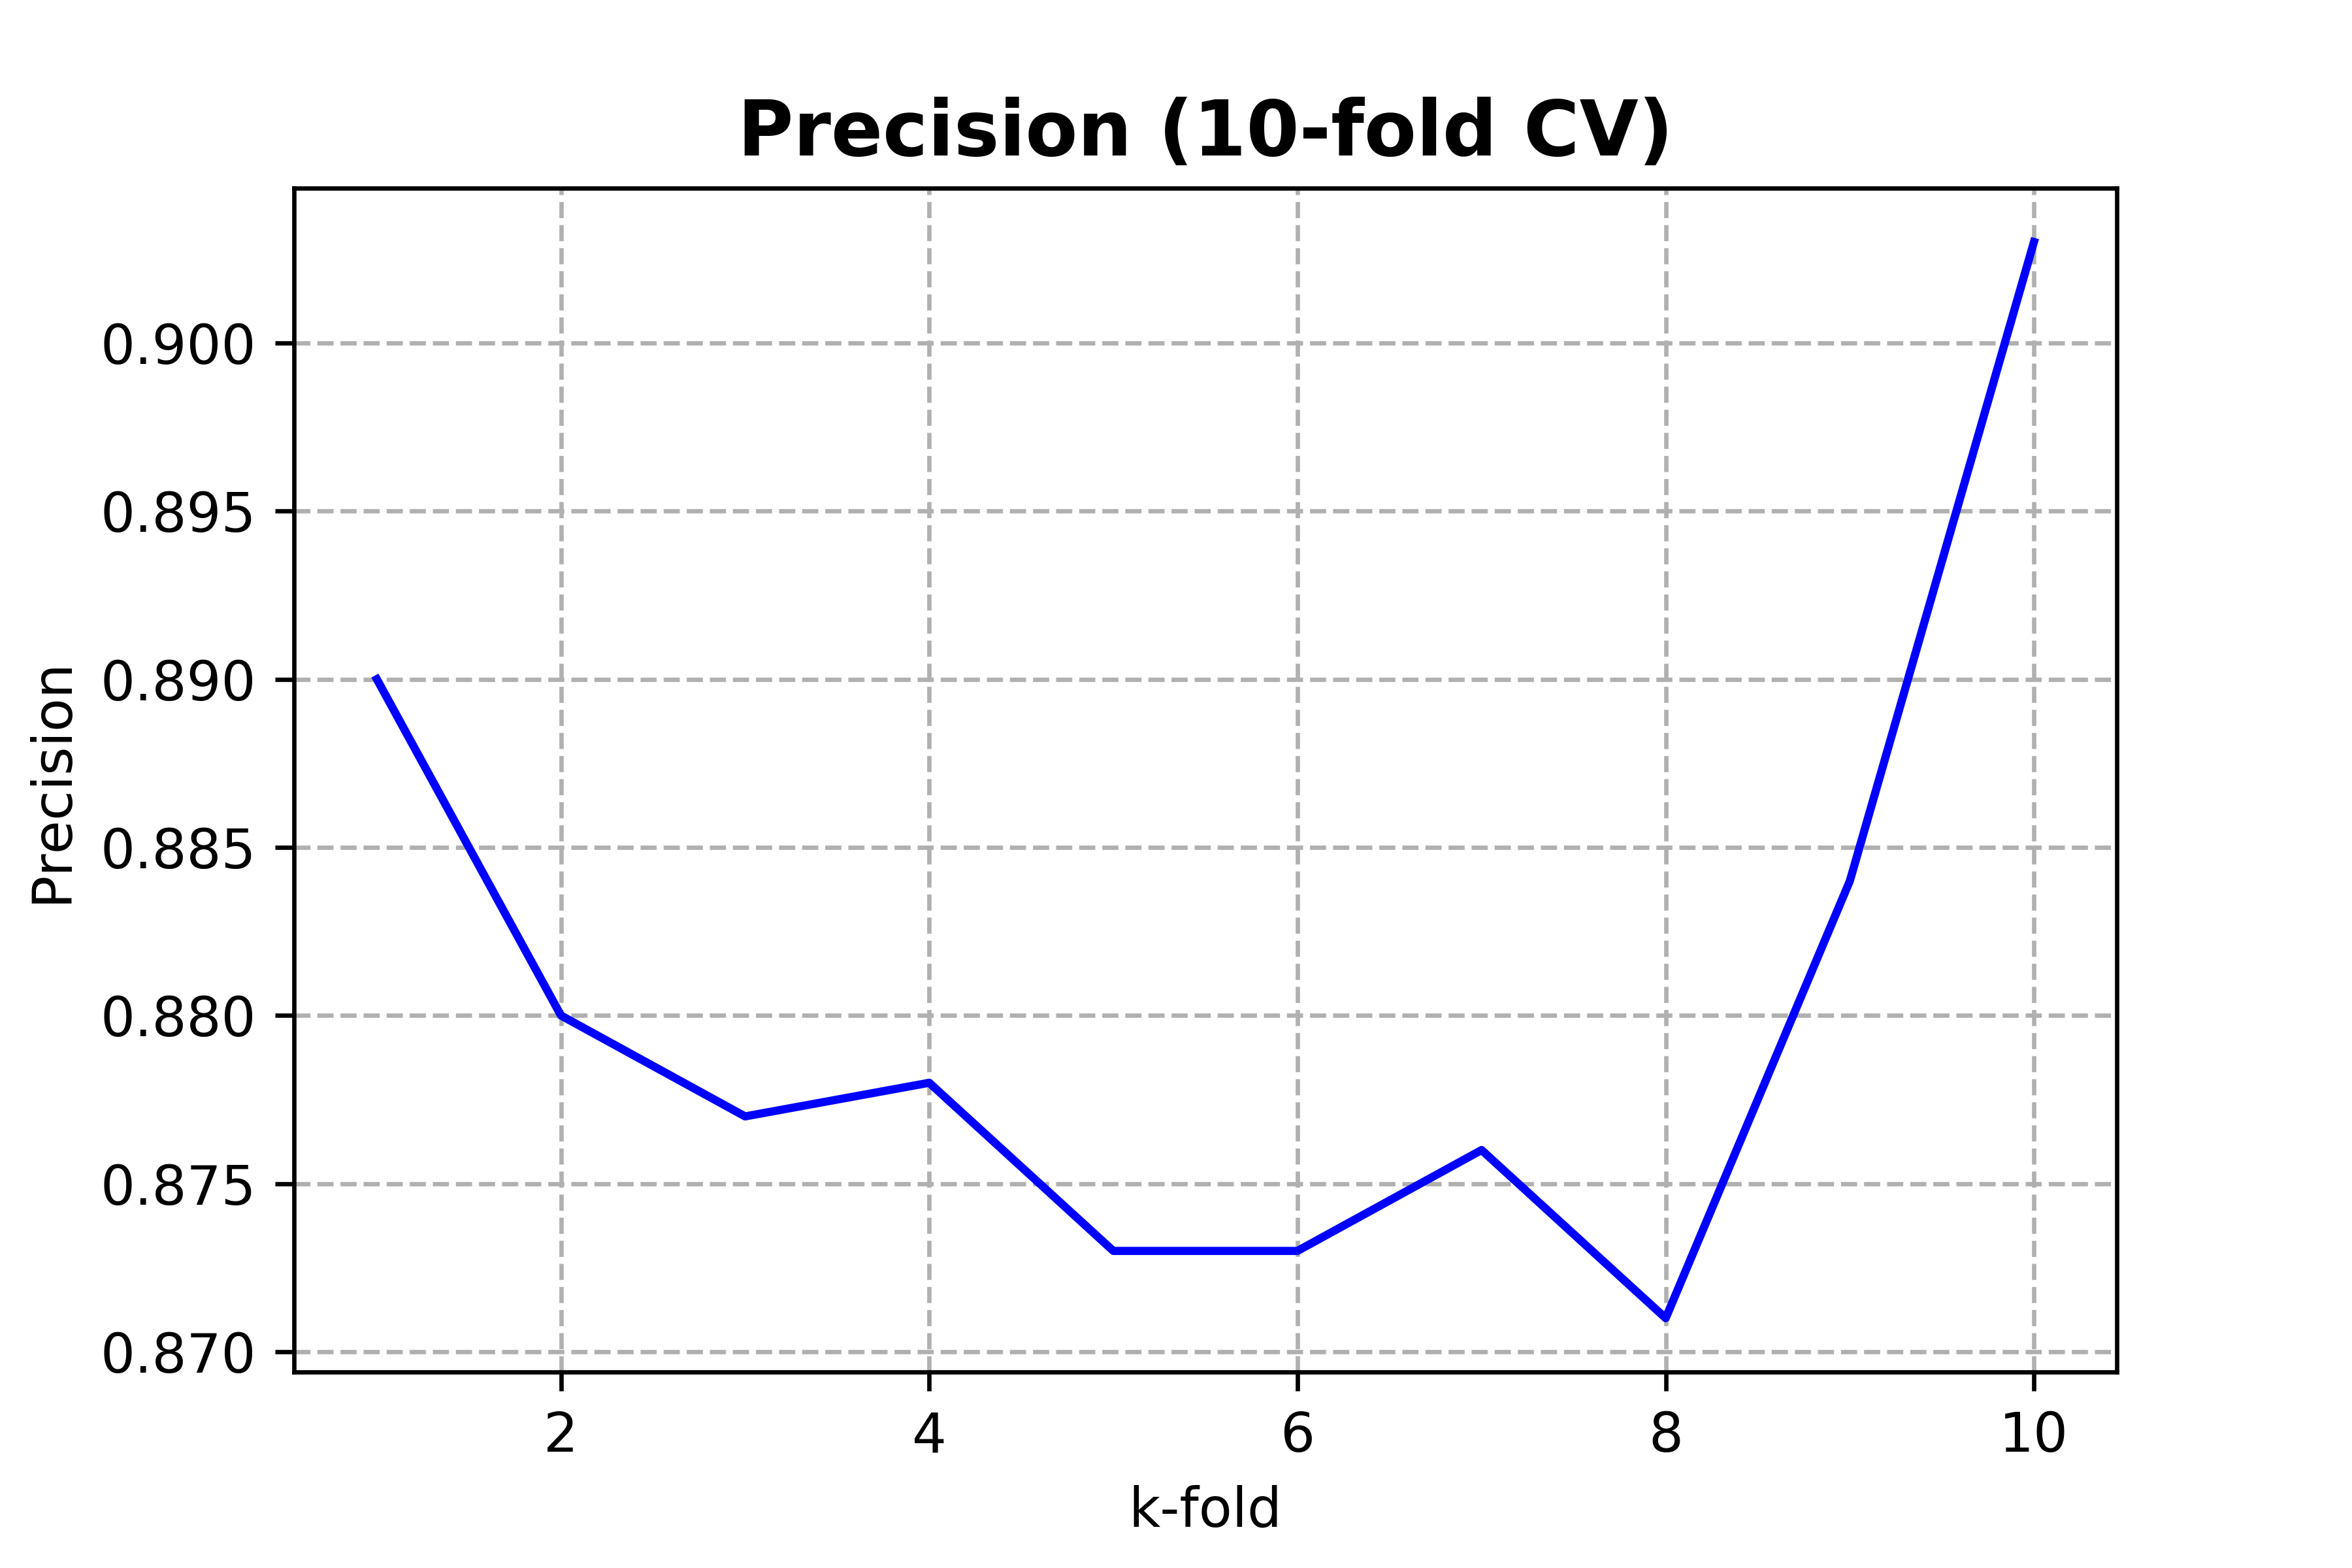
\includegraphics[width=0.45\linewidth]{figures/precision_nn_tuned.png} 
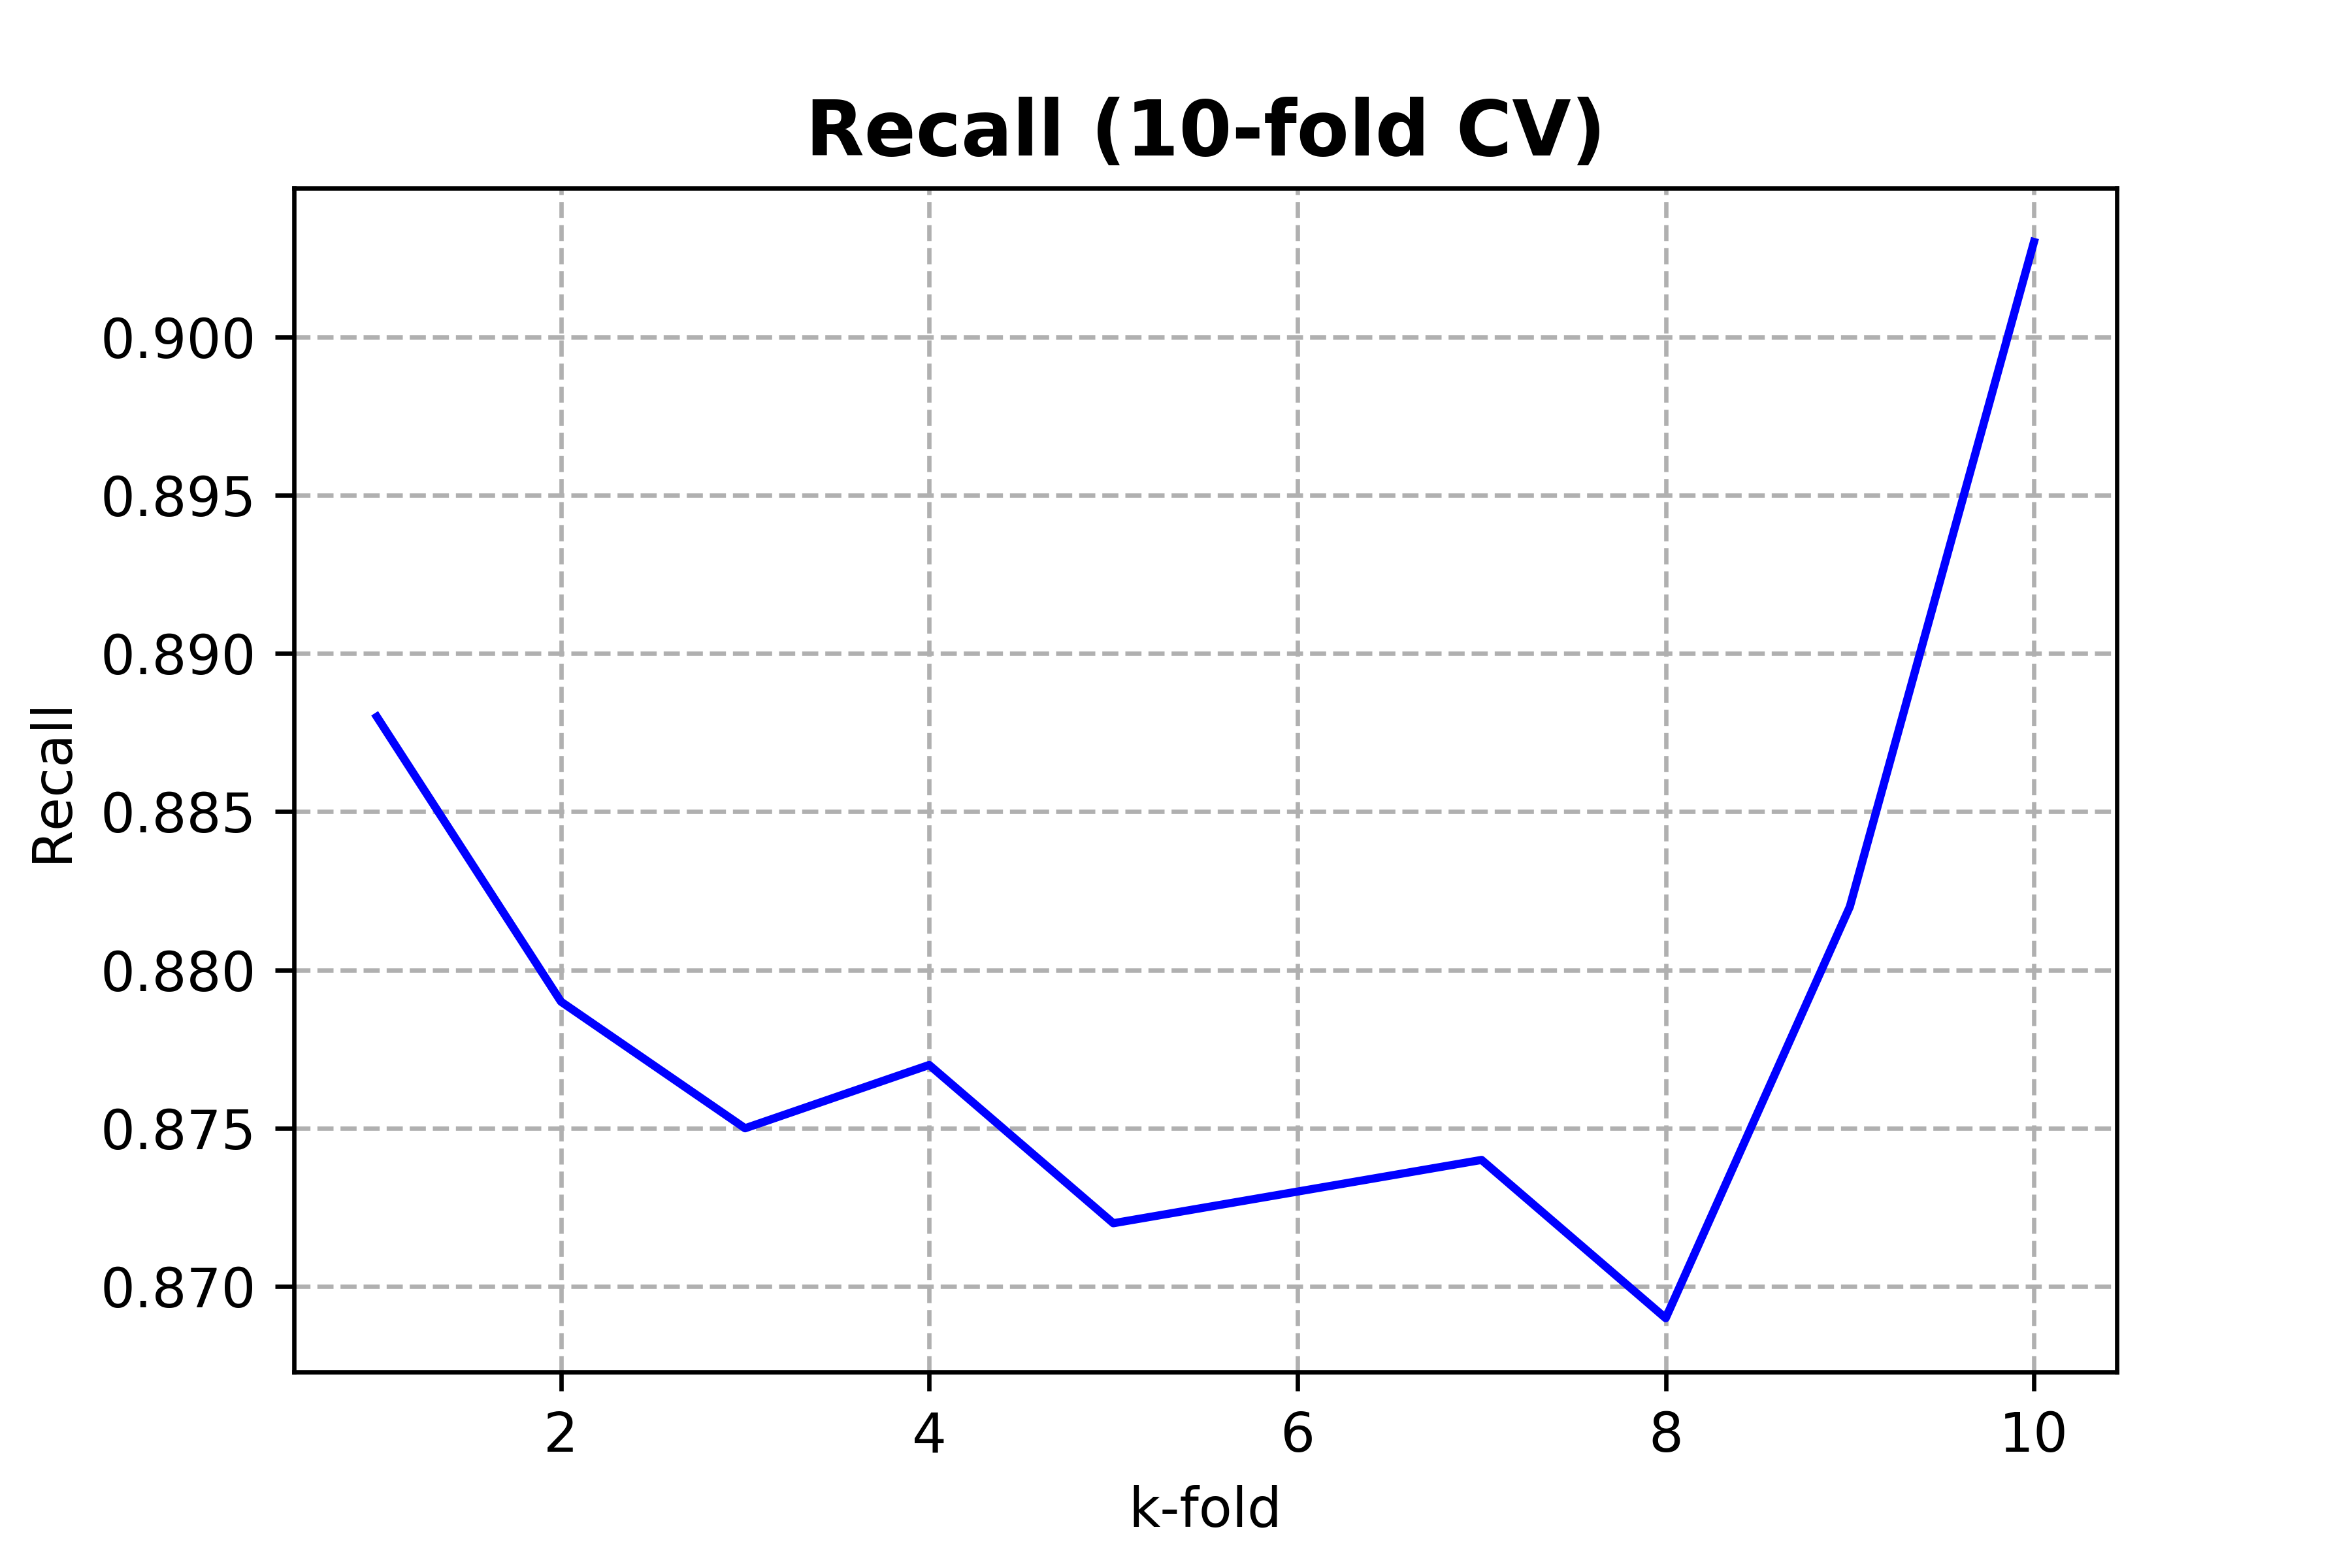
\includegraphics[width=0.45\linewidth]{figures/recall_nn_tuned.png}
\caption{(Left) Precision curve. (Right) Recall curve. [Hypothesis test NN with PCA] \label{fig:hypo_pca_nn_pre_recl}}
\end{figure}

\item{\textbf{K-Nearest Neighbors.}} The results for the Hypothesis run for KNN is shown in Figs . The results can be compared to the SVM and NN runs and it is obvious that the KNN performs better than both the SVM and NN from a look at the plots for both. This is reflected in the hypothesis result table \ref{tab:hypo_test_pca}.

\begin{figure}[H]
\centering
\includegraphics[width=0.45\linewidth]{figures/{KNN_ROC_K_3_fold_1_using_pca}.pdf} 
\includegraphics[width=0.5\linewidth]{figures/{KNN_Conf_matrix_k_3_fold_1_using_pca}.pdf}
\caption{(Left) ROC curve. (Right) Confusion matrix [Hypothesis test KNN with PCA] \label{fig:hypo_pca_knn_roc_conf}}
\end{figure}

\begin{figure}[H]
\centering
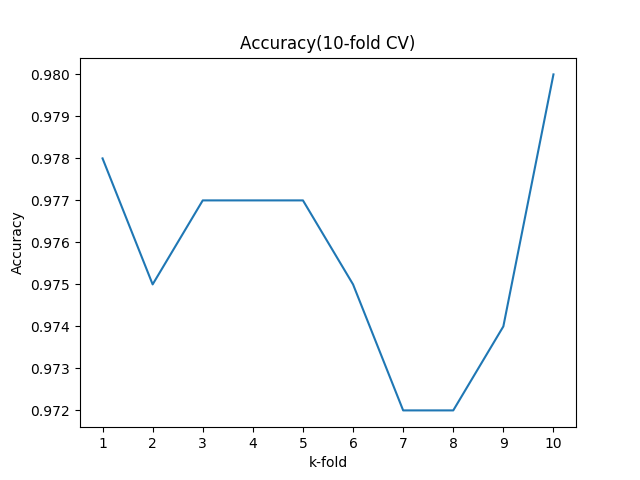
\includegraphics[width=0.5\linewidth]{figures/accuracy_knn_PCA.png}
\caption{Accurcay (KNN) over the 10-fold CV (Hypothesis testing - with PCA). \label{fig:acc_knn_hypo_pca}}
\end{figure}

\begin{figure}[H]
\centering
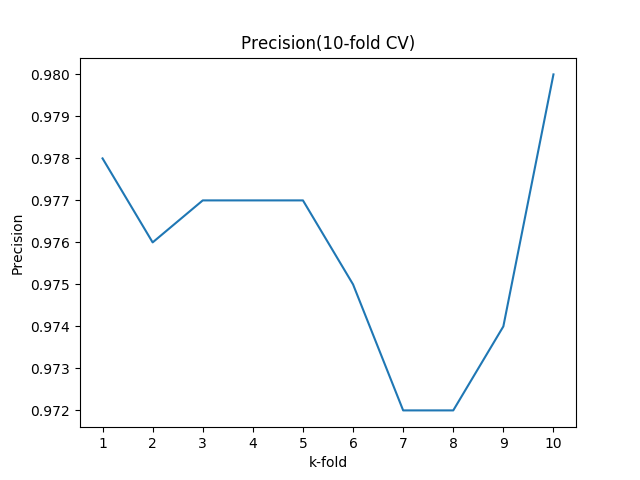
\includegraphics[width=0.45\linewidth]{figures/precision_knn.png} 
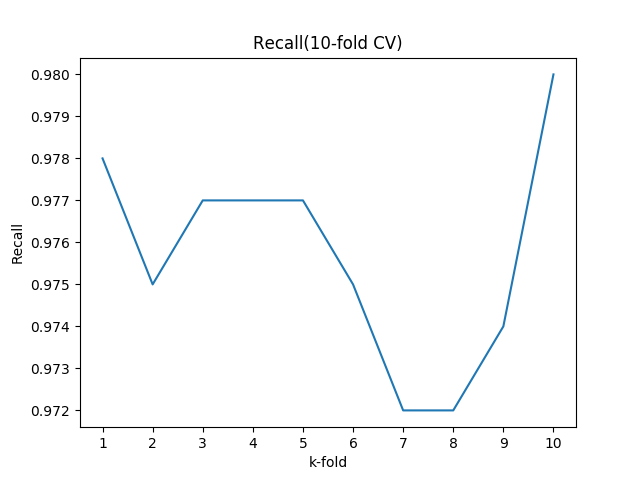
\includegraphics[width=0.45\linewidth]{figures/recall_knn.png}
\caption{(Left) Precision curve. (Right) Recall curve. [Hypothesis test KNN with PCA] \label{fig:hypo_pca_knn_pre_recl}}
\end{figure}

\end{itemize}

\addcontentsline{toc}{subsubsection}{Comparison using actual data}
\subsubsection*{Comparison using actual data}

The same set of experiments mentioned above were performed using the actual data without any pre-processing and are shown in the following sections for all the three algorithms. These data were used to perform Hypothesis testing for all combinations of algorithms and the results can be seen in the table below:

\begin{table}[H] 
\centering
\begin{tabular}{ c|c|c }
 \textbf{Experiment} & \textbf{Result} & \textbf{Inference} \\ 
 \hline
Neural Net vs. SVM & $x < x_{\alpha}$ & Equal ($\mu_{NN} = \mu_{SVM}$) Accept Null Hypothesis\\ 
KNN vs. SVM & $x > x_{\alpha}$ &  KNN ($\mu_{KNN} > \mu_{SVM}$) Reject Null Hypothesis\\ 
KNN vs. Neural Net & $x > x_{\alpha}$ &  KNN ($\mu_{KNN} > \mu_{NN}$) Reject Null Hypothesis \\
\end{tabular}
\caption{Hypothesis testing results (without PCA) \label{tab:hypo_test_actual}}
\end{table}

\paragraph{Observations.}

\begin{itemize}
\item{\textbf{Support Vector Machine.}} The results for the Hypothesis run for SVM with the actual data is shown in Fig \ref{fig:hypo_svm_roc_acc_act}.

\begin{figure}[H]
\centering
\includegraphics[width=0.45\linewidth]{figures/{SVM_linear_ROC_C_70.0_k_1}.png} 
\includegraphics[width=0.45\linewidth]{figures/acc_svm_tuned_without_pca_hypo.png}
\caption{(Left) ROC curve. (Right) Accuracy curve. [Hypothesis test SVM without PCA] \label{fig:hypo_svm_roc_acc_act}}
\end{figure}

\item{\textbf{Neural Network.}} The results for the Hypothesis run for NN with the actual data is shown in Fig \ref{fig:hypo_nn_roc_acc_act}.

\begin{figure}[H]
\centering
\includegraphics[width=0.45\linewidth]{figures/{Neural_Net_linear_ROC_Alpha_100_Act_fcn_logistic_Learn_rate_0.002_k_1}.png} 
\includegraphics[width=0.45\linewidth]{figures/acc_nn_tuned_without_pca_hypo.png}
\caption{(Left) ROC curve. (Right) Accuracy curve. [Hypothesis test NN without PCA] \label{fig:hypo_nn_roc_acc_act}}
\end{figure}

\item{\textbf{K-Nearest Neighbor.}} The results for the Hypothesis run for KNN with the actual data is shown in Fig \ref{fig:hypo_knn_roc_acc_act}.

\begin{figure}[H]
\centering
\includegraphics[width=0.45\linewidth]{figures/KNN_ROC_K_3_fold_1.pdf} 
\includegraphics[width=0.45\linewidth]{figures/accuracy_knn_without_PCA.png}
\caption{(Left) ROC curve. (Right) Accuracy curve. [Hypothesis test KNN without PCA] \label{fig:hypo_knn_roc_acc_act}}
\end{figure}

\end{itemize}

\addcontentsline{toc}{subsubsection}{Within algorithm comparison}
\subsubsection*{Within algorithm comparison}

Apart from the above comparisons, we performed hypothesis tests to compare the performance of these algorithms using PCA data vs. using the actual data. The results from these experiments are shown below. 

\begin{table}[H] 
\centering
\begin{tabular}{ c|c|c }
 \textbf{Experiment} & \textbf{Result} & \textbf{Inference} \\ 
 \hline
SVM (actual) vs. & $x > x_{\alpha}$ & SVM (actual data) ($\mu_{SVM\_actual} > \mu_{SVM\_pca}$) \\ 
SVM (with PCA) & & Reject Null Hypothesis \\ 
& & \\
Neural Net (actual) vs. & $x < x_{\alpha}$ &  Equal ($\mu_{NN\_pca} = \mu_{NN\_actual}$) \\
Neural Net (with PCA)  & & Accept Null Hypothesis\\ 
& & \\
KNN (actual) vs. & $x < x_{\alpha}$ &  Equal ($\mu_{KNN\_pca} = \mu_{KNN\_actual}$) \\
KNN (with PCA)  & & Accept Null Hypothesis\\ 
\end{tabular}
\caption{Hypothesis testing with PCA vs. without PCA \label{tab:hypo_pca_vs_act}}
\end{table}
 
The results above show that while SVM performs better using the actual data, using Neural Network and KNN with PCA data produces similar performance as using the actual data. This provides a lot of flexibility in selecting the algorithm because using PCA data reduces the training time a lot. 
 
\end{document}


